\documentclass[twoside]{book}

% Packages required by doxygen
\usepackage{fixltx2e}
\usepackage{calc}
\usepackage{doxygen}
\usepackage{graphicx}
\usepackage[utf8]{inputenc}
\usepackage{makeidx}
\usepackage{multicol}
\usepackage{multirow}
\PassOptionsToPackage{warn}{textcomp}
\usepackage{textcomp}
\usepackage[nointegrals]{wasysym}
\usepackage[table]{xcolor}

% Font selection
\usepackage[T1]{fontenc}
\usepackage{mathptmx}
\usepackage[scaled=.90]{helvet}
\usepackage{courier}
\usepackage{amssymb}
\usepackage{sectsty}
\renewcommand{\familydefault}{\sfdefault}
\allsectionsfont{%
  \fontseries{bc}\selectfont%
  \color{darkgray}%
}
\renewcommand{\DoxyLabelFont}{%
  \fontseries{bc}\selectfont%
  \color{darkgray}%
}
\newcommand{\+}{\discretionary{\mbox{\scriptsize$\hookleftarrow$}}{}{}}

% Page & text layout
\usepackage{geometry}
\geometry{%
  a4paper,%
  top=2.5cm,%
  bottom=2.5cm,%
  left=2.5cm,%
  right=2.5cm%
}
\tolerance=750
\hfuzz=15pt
\hbadness=750
\setlength{\emergencystretch}{15pt}
\setlength{\parindent}{0cm}
\setlength{\parskip}{0.2cm}
\makeatletter
\renewcommand{\paragraph}{%
  \@startsection{paragraph}{4}{0ex}{-1.0ex}{1.0ex}{%
    \normalfont\normalsize\bfseries\SS@parafont%
  }%
}
\renewcommand{\subparagraph}{%
  \@startsection{subparagraph}{5}{0ex}{-1.0ex}{1.0ex}{%
    \normalfont\normalsize\bfseries\SS@subparafont%
  }%
}
\makeatother

% Headers & footers
\usepackage{fancyhdr}
\pagestyle{fancyplain}
\fancyhead[LE]{\fancyplain{}{\bfseries\thepage}}
\fancyhead[CE]{\fancyplain{}{}}
\fancyhead[RE]{\fancyplain{}{\bfseries\leftmark}}
\fancyhead[LO]{\fancyplain{}{\bfseries\rightmark}}
\fancyhead[CO]{\fancyplain{}{}}
\fancyhead[RO]{\fancyplain{}{\bfseries\thepage}}
\fancyfoot[LE]{\fancyplain{}{}}
\fancyfoot[CE]{\fancyplain{}{}}
\fancyfoot[RE]{\fancyplain{}{\bfseries\scriptsize Generated on Mon Jul 4 2016 17\+:05\+:31 for Doxygen-\/\+Documentation by Doxygen }}
\fancyfoot[LO]{\fancyplain{}{\bfseries\scriptsize Generated on Mon Jul 4 2016 17\+:05\+:31 for Doxygen-\/\+Documentation by Doxygen }}
\fancyfoot[CO]{\fancyplain{}{}}
\fancyfoot[RO]{\fancyplain{}{}}
\renewcommand{\footrulewidth}{0.4pt}
\renewcommand{\chaptermark}[1]{%
  \markboth{#1}{}%
}
\renewcommand{\sectionmark}[1]{%
  \markright{\thesection\ #1}%
}

% Indices & bibliography
\usepackage{natbib}
\usepackage[titles]{tocloft}
\setcounter{tocdepth}{3}
\setcounter{secnumdepth}{5}
\makeindex

% Hyperlinks (required, but should be loaded last)
\usepackage{ifpdf}
\ifpdf
  \usepackage[pdftex,pagebackref=true]{hyperref}
\else
  \usepackage[ps2pdf,pagebackref=true]{hyperref}
\fi
\hypersetup{%
  colorlinks=true,%
  linkcolor=blue,%
  citecolor=blue,%
  unicode%
}

% Custom commands
\newcommand{\clearemptydoublepage}{%
  \newpage{\pagestyle{empty}\cleardoublepage}%
}


%===== C O N T E N T S =====

\begin{document}

% Titlepage & ToC
\hypersetup{pageanchor=false,
             bookmarks=true,
             bookmarksnumbered=true,
             pdfencoding=unicode
            }
\pagenumbering{roman}
\begin{titlepage}
\vspace*{7cm}
\begin{center}%
{\Large Doxygen-\/\+Documentation }\\
\vspace*{1cm}
{\large Generated by Doxygen 1.8.7}\\
\vspace*{0.5cm}
{\small Mon Jul 4 2016 17:05:31}\\
\end{center}
\end{titlepage}
\clearemptydoublepage
\tableofcontents
\clearemptydoublepage
\pagenumbering{arabic}
\hypersetup{pageanchor=true}

%--- Begin generated contents ---
\chapter{$<$h1$>$Introduction$<$/h1$>$}
\label{index}\hypertarget{index}{}This is the doxy generated documentation of the \href{https://github.com/joseluisquiroga/ben-jose}{\tt Ben-\/\+Jose} Trainable S\+AT Solver Library. It is not a complete reference of all the classes and functions. It is a selection of the most releveant classes and functions that help in the understanding of the innerworkig of the library.

The \hyperlink{group__docgrp___a_p_i}{User\textquotesingle{}s A\+PI} of the library is implemented in the files \hyperlink{ben__jose_8cpp}{ben\+\_\+jose.\+cpp} and \hyperlink{ben__jose_8h}{ben\+\_\+jose.\+h}, and documented in\+:


\begin{DoxyItemize}
\item \hyperlink{group__docgrp___a_p_i}{User\textquotesingle{}s A\+PI} 
\end{DoxyItemize}

The architecture of the ben-\/jose library is strongly monolitic in the sense that the basic functionality of the whole library is basically one function (\hyperlink{classbrain_a2daa8c1c03eea62a51a359470bb64cc7}{brain\+::solve\+\_\+instance}) with three presentations\+:


\begin{DoxyItemize}
\item \hyperlink{ben__jose_8h_a65eb23939cc4ae39654dbd93343580c8}{bj\+\_\+solve\+\_\+file} 
\item \hyperlink{ben__jose_8h_a45eef575a2ca6c6b90e0a1d998f1eb7d}{bj\+\_\+solve\+\_\+data} 
\item \hyperlink{ben__jose_8h_a2818f32df95b8d462f49a201ce371142}{bj\+\_\+solve\+\_\+literals} 
\end{DoxyItemize}

That means that every piece of code within the \textquotesingle{}library\textquotesingle{} directory of the source tree is tightly coupled. Having said that, this documentations should give a good idea of it\textquotesingle{}s architecture.

The most relevant classes of the library implementation can be grouped as\+:


\begin{DoxyItemize}
\item \hyperlink{group__docgrp___c_d_c_l__classes}{D\+P\+L\+L+\+B\+C\+P+\+C\+D\+CL classes} 
\item \hyperlink{group__docgrp__stab__classes}{Stabilization classes} 
\item \hyperlink{group__docgrp__matching__classes}{Matching classes} 
\item \hyperlink{group__docgrp__database__classes}{Database classes} 
\end{DoxyItemize}

The macro behavior of the innerwork of the library is described in\+:


\begin{DoxyItemize}
\item \hyperlink{macro__algorithm__ben__jose_8cpp}{macro\+\_\+algorithm\+\_\+ben\+\_\+jose.\+cpp} 
\end{DoxyItemize}
\chapter{Module Index}
\section{Modules}
Here is a list of all modules\+:\begin{DoxyCompactList}
\item \contentsline{section}{User's A\+P\+I}{\pageref{d1/db8/group__docgrp___a_p_i}}{}
\item \contentsline{section}{D\+P\+L\+L+\+B\+C\+P+\+C\+D\+C\+L classes}{\pageref{dc/df2/group__docgrp___c_d_c_l__classes}}{}
\item \contentsline{section}{Stabilization classes}{\pageref{d1/dbe/group__docgrp__stab__classes}}{}
\item \contentsline{section}{Matching classes}{\pageref{d2/dbb/group__docgrp__matching__classes}}{}
\item \contentsline{section}{Database classes}{\pageref{d9/d24/group__docgrp__database__classes}}{}
\end{DoxyCompactList}

\chapter{Class Index}
\section{Class List}
Here are the classes, structs, unions and interfaces with brief descriptions\+:\begin{DoxyCompactList}
\item\contentsline{section}{\hyperlink{classbrain}{brain} \\*Class that holds all data used to solve a particular C\+NF instance }{\pageref{d7/d79/classbrain}}{}
\item\contentsline{section}{\hyperlink{classcanon__cnf}{canon\+\_\+cnf} \\*A \hyperlink{classcanon__cnf}{canon\+\_\+cnf} is a B\+C\+FF. An stabilized sub-\/formula }{\pageref{da/deb/classcanon__cnf}}{}
\item\contentsline{section}{\hyperlink{classcoloring}{coloring} \\*The initial and final state for an stabilization is a coloring }{\pageref{d2/d9a/classcoloring}}{}
\item\contentsline{section}{\hyperlink{classdeducer}{deducer} \\*Class that holds the data used to analyze a conflict }{\pageref{d7/d0b/classdeducer}}{}
\item\contentsline{section}{\hyperlink{classdeduction}{deduction} \\*Class that holds the result of analyzing (doing resolution) of a conflict }{\pageref{d3/df3/classdeduction}}{}
\item\contentsline{section}{\hyperlink{classinstance__info}{instance\+\_\+info} \\*Class that holds an instance data }{\pageref{dc/dd0/classinstance__info}}{}
\item\contentsline{section}{\hyperlink{classleveldat}{leveldat} \\*Class that holds the data of a level }{\pageref{df/da3/classleveldat}}{}
\item\contentsline{section}{\hyperlink{classneuromap}{neuromap} \\*A neuromap is a C\+NF sub-\/formula }{\pageref{d6/d45/classneuromap}}{}
\item\contentsline{section}{\hyperlink{classneuron}{neuron} \\*Class for C\+NF clause behavior. So there is one neuron per clause }{\pageref{d9/d00/classneuron}}{}
\item\contentsline{section}{\hyperlink{classprop__signal}{prop\+\_\+signal} \\*Class for representing B\+CP propagation data }{\pageref{d8/df2/classprop__signal}}{}
\item\contentsline{section}{\hyperlink{classquanton}{quanton} \\*Class for C\+NF variables (each variable has a positon and a negaton) }{\pageref{de/df5/classquanton}}{}
\item\contentsline{section}{\hyperlink{structsha2__context}{sha2\+\_\+context} \\*S\+H\+A-\/256 context structure }{\pageref{d0/d04/structsha2__context}}{}
\item\contentsline{section}{\hyperlink{classskeleton__glb}{skeleton\+\_\+glb} \\*A \hyperlink{classskeleton__glb}{skeleton\+\_\+glb} is a directory holding a database }{\pageref{dd/dad/classskeleton__glb}}{}
\item\contentsline{section}{\hyperlink{classsorset}{sorset} \\*A sorset is a group of \hyperlink{classsortee}{sortee} s }{\pageref{d3/d62/classsorset}}{}
\item\contentsline{section}{\hyperlink{classsort__glb}{sort\+\_\+glb} \\*Class that holds all global data used to stabilize a group of items }{\pageref{d7/dec/classsort__glb}}{}
\item\contentsline{section}{\hyperlink{classsortee}{sortee} \\*Class that is an item to be stabilized }{\pageref{d8/d36/classsortee}}{}
\item\contentsline{section}{\hyperlink{classsortrel}{sortrel} \\*A sortrel is a relation between two \hyperlink{classsortee}{sortee} s }{\pageref{d6/de7/classsortrel}}{}
\end{DoxyCompactList}

\chapter{File Index}
\section{File List}
Here is a list of all documented files with brief descriptions\+:\begin{DoxyCompactList}
\item\contentsline{section}{/home/jose/devel/ben-\/jose/src/external/{\bfseries bj\+\_\+big\+\_\+number.\+h} }{\pageref{d6/d1e/bj__big__number_8h}}{}
\item\contentsline{section}{/home/jose/devel/ben-\/jose/src/external/{\bfseries bj\+\_\+mem.\+h} }{\pageref{d6/d5a/bj__mem_8h}}{}
\item\contentsline{section}{/home/jose/devel/ben-\/jose/src/external/{\bfseries bj\+\_\+proc.\+h} }{\pageref{de/d6d/bj__proc_8h}}{}
\item\contentsline{section}{/home/jose/devel/ben-\/jose/src/external/{\bfseries bj\+\_\+stream.\+h} }{\pageref{d4/dc7/bj__stream_8h}}{}
\item\contentsline{section}{/home/jose/devel/ben-\/jose/src/external/{\bfseries bj\+\_\+time.\+h} }{\pageref{d2/d72/bj__time_8h}}{}
\item\contentsline{section}{/home/jose/devel/ben-\/jose/src/external/{\bfseries ch\+\_\+string.\+h} }{\pageref{d0/df6/ch__string_8h}}{}
\item\contentsline{section}{/home/jose/devel/ben-\/jose/src/external/{\bfseries platform.\+h} }{\pageref{de/d03/platform_8h}}{}
\item\contentsline{section}{/home/jose/devel/ben-\/jose/src/external/{\bfseries stack\+\_\+trace.\+h} }{\pageref{d7/d4c/stack__trace_8h}}{}
\item\contentsline{section}{/home/jose/devel/ben-\/jose/src/external/{\bfseries top\+\_\+exception.\+h} }{\pageref{d5/d9a/top__exception_8h}}{}
\item\contentsline{section}{/home/jose/devel/ben-\/jose/src/library/api/\hyperlink{ben__jose_8cpp}{ben\+\_\+jose.\+cpp} \\*File containing the implementation code for the users A\+P\+I of ben\+\_\+jose }{\pageref{d1/d55/ben__jose_8cpp}}{}
\item\contentsline{section}{/home/jose/devel/ben-\/jose/src/library/api/\hyperlink{ben__jose_8h}{ben\+\_\+jose.\+h} \\*Ben\+\_\+jose A\+P\+I declaration }{\pageref{dc/d3c/ben__jose_8h}}{}
\item\contentsline{section}{/home/jose/devel/ben-\/jose/src/library/brain/\hyperlink{brain_8h}{brain.\+h} \\*Declarations of classes and that implement the solver's core functionality }{\pageref{db/d3c/brain_8h}}{}
\item\contentsline{section}{/home/jose/devel/ben-\/jose/src/library/brain/{\bfseries instance\+\_\+info.\+h} }{\pageref{d1/d4a/instance__info_8h}}{}
\item\contentsline{section}{/home/jose/devel/ben-\/jose/src/library/brain/{\bfseries solver.\+h} }{\pageref{d4/d20/solver_8h}}{}
\item\contentsline{section}{/home/jose/devel/ben-\/jose/src/library/brain/{\bfseries sortor.\+h} }{\pageref{d7/dd0/sortor_8h}}{}
\item\contentsline{section}{/home/jose/devel/ben-\/jose/src/library/brain/{\bfseries str\+\_\+set.\+h} }{\pageref{d1/de7/str__set_8h}}{}
\item\contentsline{section}{/home/jose/devel/ben-\/jose/src/library/debug/{\bfseries dbg\+\_\+config.\+h} }{\pageref{d7/dc5/dbg__config_8h}}{}
\item\contentsline{section}{/home/jose/devel/ben-\/jose/src/library/debug/{\bfseries dbg\+\_\+prt.\+h} }{\pageref{d1/db7/dbg__prt_8h}}{}
\item\contentsline{section}{/home/jose/devel/ben-\/jose/src/library/debug/{\bfseries dbg\+\_\+run\+\_\+satex.\+h} }{\pageref{da/d19/dbg__run__satex_8h}}{}
\item\contentsline{section}{/home/jose/devel/ben-\/jose/src/library/debug/{\bfseries dbg\+\_\+sortor.\+h} }{\pageref{d1/de4/dbg__sortor_8h}}{}
\item\contentsline{section}{/home/jose/devel/ben-\/jose/src/library/dimacs/{\bfseries dimacs.\+h} }{\pageref{d1/dd7/dimacs_8h}}{}
\item\contentsline{section}{/home/jose/devel/ben-\/jose/src/library/shuffler/{\bfseries shuffler.\+h} }{\pageref{d2/d89/shuffler_8h}}{}
\item\contentsline{section}{/home/jose/devel/ben-\/jose/src/library/unsat\+\_\+db/{\bfseries html\+\_\+strings.\+h} }{\pageref{d0/d96/html__strings_8h}}{}
\item\contentsline{section}{/home/jose/devel/ben-\/jose/src/library/unsat\+\_\+db/{\bfseries proof.\+h} }{\pageref{d4/dff/proof_8h}}{}
\item\contentsline{section}{/home/jose/devel/ben-\/jose/src/library/unsat\+\_\+db/{\bfseries skeleton.\+h} }{\pageref{d4/dcf/skeleton_8h}}{}
\item\contentsline{section}{/home/jose/devel/ben-\/jose/src/programs/macro\+\_\+ben\+\_\+jose/\hyperlink{macro__algorithm__ben__jose_8cpp}{macro\+\_\+algorithm\+\_\+ben\+\_\+jose.\+cpp} \\*This is a documentation file to help understand the innerworking of the library. It is not compiled }{\pageref{d0/d6d/macro__algorithm__ben__jose_8cpp}}{}
\item\contentsline{section}{/home/jose/devel/ben-\/jose/src/programs/tests/phi/{\bfseries phi\+\_\+test.\+h} }{\pageref{db/d1b/phi__test_8h}}{}
\item\contentsline{section}{/home/jose/devel/ben-\/jose/src/programs/tests/solver/{\bfseries batch\+\_\+solver.\+h} }{\pageref{dc/d4d/batch__solver_8h}}{}
\item\contentsline{section}{/home/jose/devel/ben-\/jose/src/utils/{\bfseries binder.\+h} }{\pageref{d3/d2f/binder_8h}}{}
\item\contentsline{section}{/home/jose/devel/ben-\/jose/src/utils/{\bfseries bit\+\_\+row.\+h} }{\pageref{dd/d61/bit__row_8h}}{}
\item\contentsline{section}{/home/jose/devel/ben-\/jose/src/utils/{\bfseries file\+\_\+funcs.\+h} }{\pageref{d8/d41/file__funcs_8h}}{}
\item\contentsline{section}{/home/jose/devel/ben-\/jose/src/utils/{\bfseries file\+\_\+tree.\+h} }{\pageref{d6/d2b/file__tree_8h}}{}
\item\contentsline{section}{/home/jose/devel/ben-\/jose/src/utils/{\bfseries mem\+\_\+redblack.\+h} }{\pageref{d6/d2e/mem__redblack_8h}}{}
\item\contentsline{section}{/home/jose/devel/ben-\/jose/src/utils/{\bfseries parse\+\_\+funcs.\+h} }{\pageref{d9/d0f/parse__funcs_8h}}{}
\item\contentsline{section}{/home/jose/devel/ben-\/jose/src/utils/{\bfseries print\+\_\+macros.\+h} }{\pageref{dd/dd9/print__macros_8h}}{}
\item\contentsline{section}{/home/jose/devel/ben-\/jose/src/utils/{\bfseries redblack.\+h} }{\pageref{d5/d56/redblack_8h}}{}
\item\contentsline{section}{/home/jose/devel/ben-\/jose/src/utils/\hyperlink{sha2_8h}{sha2.\+h} }{\pageref{db/d4d/sha2_8h}}{}
\item\contentsline{section}{/home/jose/devel/ben-\/jose/src/utils/{\bfseries tak\+\_\+mak.\+h} }{\pageref{d6/d34/tak__mak_8h}}{}
\item\contentsline{section}{/home/jose/devel/ben-\/jose/src/utils/{\bfseries tools.\+h} }{\pageref{d5/da5/tools_8h}}{}
\item\contentsline{section}{/home/jose/devel/ben-\/jose/src/utils/{\bfseries util\+\_\+funcs.\+h} }{\pageref{d0/d5a/util__funcs_8h}}{}
\end{DoxyCompactList}

\chapter{Module Documentation}
\hypertarget{group__docgrp___a_p_i}{}\section{User\textquotesingle{}s A\+PI}
\label{group__docgrp___a_p_i}\index{User\textquotesingle{}s A\+PI@{User\textquotesingle{}s A\+PI}}
\subsection*{Enumerations}


\subsection{Detailed Description}
The basic interaction is best described by the bj-\/hello-\/world.\+c program


\begin{DoxyCodeInclude}

\textcolor{preprocessor}{#include <stdio.h>}
\textcolor{preprocessor}{#include "\hyperlink{ben__jose_8h}{ben\_jose.h}"}

\textcolor{keywordtype}{int} main(\textcolor{keywordtype}{int} argc, \textcolor{keywordtype}{char}** argv)
\{
    \textcolor{keywordflow}{if}(argc < 2)\{
        printf(\textcolor{stringliteral}{"args: <cnf\_file\_path> [<db\_dir>]\(\backslash\)n"});
        \textcolor{keywordflow}{return} 1;
    \}
    \textcolor{keywordtype}{char}* dd = \textcolor{stringliteral}{"."};
    \textcolor{keywordtype}{char}* ff = argv[1];
    \textcolor{keywordflow}{if}(argc > 2)\{
        dd = argv[2];
    \}
    
    \hyperlink{ben__jose_8h_a3825fe3519107001ca4d0679f1d0a110}{bj\_solver\_t} ss = \hyperlink{ben__jose_8cpp_a3f6cb5e5aac2da12b2d475c81909becf}{bj\_solver\_create}(dd);
    
    \hyperlink{group__docgrp___a_p_i_ga9aba221730ab694a549d25ee1aa28c69}{bj\_satisf\_val\_t}  vv = \hyperlink{ben__jose_8cpp_a65eb23939cc4ae39654dbd93343580c8}{bj\_solve\_file}(ss, ff);
    \textcolor{keywordflow}{switch}(vv)\{
        \textcolor{keywordflow}{case} \hyperlink{ben__jose_8h_ga9aba221730ab694a549d25ee1aa28c69af4c1851202dc8838008241c2a527a069}{bjr\_yes\_satisf}:
            printf(\textcolor{stringliteral}{"%s is SAT instance\(\backslash\)n"}, ff);
            \textcolor{keywordflow}{break};
        \textcolor{keywordflow}{case} \hyperlink{ben__jose_8h_ga9aba221730ab694a549d25ee1aa28c69adc2a37bfd4482eb5167ebb9d47245e8b}{bjr\_no\_satisf}:
            printf(\textcolor{stringliteral}{"%s is UNS instance\(\backslash\)n"}, ff);
            \textcolor{keywordflow}{break};
        \textcolor{keywordflow}{case} \hyperlink{ben__jose_8h_ga9aba221730ab694a549d25ee1aa28c69a5cee678e06286f3dd31c2f8d60e88979}{bjr\_error}:
            \{
                printf(\textcolor{stringliteral}{"ERROR ! in %s\(\backslash\)n"}, ff);
                bj\_output\_t oo = \hyperlink{ben__jose_8cpp_a2685b092d0a891b280bc1895d1deaef1}{bj\_get\_output}(ss);
                \textcolor{keyword}{const} \textcolor{keywordtype}{char}* e\_str = \hyperlink{ben__jose_8cpp_ab6303f60ba14cddd8b534b40830df31d}{bj\_error\_str}(oo.bjo\_error);
                printf(\textcolor{stringliteral}{"%s\(\backslash\)n"}, e\_str);
            \}
            \textcolor{keywordflow}{break};
        \textcolor{keywordflow}{default}:
            printf(\textcolor{stringliteral}{"FATAL ERROR ! in %s\(\backslash\)n"}, ff);
            \textcolor{keywordflow}{break};
    \}
    
    \textcolor{comment}{// more info with this functions}
    \textcolor{comment}{//bj\_output\_t oo = bj\_get\_output(ss);}
    \textcolor{comment}{//const long* aa = bj\_get\_assig(ss);}
    
    \hyperlink{ben__jose_8cpp_ae256ffb1a6f33249d57c88ad79c5132b}{bj\_solver\_release}(ss);
    \textcolor{keywordflow}{return} 0;
\}

\end{DoxyCodeInclude}


\subsection{Enumeration Type Documentation}
\index{User\textquotesingle{}s A\+PI@{User\textquotesingle{}s A\+PI}!bj\+\_\+satisf\+\_\+val\+\_\+t@{bj\+\_\+satisf\+\_\+val\+\_\+t}}
\index{bj\+\_\+satisf\+\_\+val\+\_\+t@{bj\+\_\+satisf\+\_\+val\+\_\+t}!User\textquotesingle{}s A\+PI@{User\textquotesingle{}s A\+PI}}
\subsubsection[{\texorpdfstring{bj\+\_\+satisf\+\_\+val\+\_\+t}{bj_satisf_val_t}}]{\setlength{\rightskip}{0pt plus 5cm}enum {\bf bj\+\_\+satisf\+\_\+val\+\_\+t}}\hypertarget{group__docgrp___a_p_i_ga9aba221730ab694a549d25ee1aa28c69}{}\label{group__docgrp___a_p_i_ga9aba221730ab694a549d25ee1aa28c69}


Posible final results of the solving process. 

\begin{Desc}
\item[Enumerator]\par
\begin{description}
\index{bjr\+\_\+unknown\+\_\+satisf@{bjr\+\_\+unknown\+\_\+satisf}!User\textquotesingle{}s A\+PI@{User\textquotesingle{}s A\+PI}}\index{User\textquotesingle{}s A\+PI@{User\textquotesingle{}s A\+PI}!bjr\+\_\+unknown\+\_\+satisf@{bjr\+\_\+unknown\+\_\+satisf}}\item[{\em 
bjr\+\_\+unknown\+\_\+satisf\hypertarget{group__docgrp___a_p_i_ga9aba221730ab694a549d25ee1aa28c69ad8dafe2640a5e989a73880526a853663}{}\label{group__docgrp___a_p_i_ga9aba221730ab694a549d25ee1aa28c69ad8dafe2640a5e989a73880526a853663}
}]Unknown result. \index{bjr\+\_\+yes\+\_\+satisf@{bjr\+\_\+yes\+\_\+satisf}!User\textquotesingle{}s A\+PI@{User\textquotesingle{}s A\+PI}}\index{User\textquotesingle{}s A\+PI@{User\textquotesingle{}s A\+PI}!bjr\+\_\+yes\+\_\+satisf@{bjr\+\_\+yes\+\_\+satisf}}\item[{\em 
bjr\+\_\+yes\+\_\+satisf\hypertarget{group__docgrp___a_p_i_ga9aba221730ab694a549d25ee1aa28c69af4c1851202dc8838008241c2a527a069}{}\label{group__docgrp___a_p_i_ga9aba221730ab694a549d25ee1aa28c69af4c1851202dc8838008241c2a527a069}
}]Satisfiable C\+NF. \index{bjr\+\_\+no\+\_\+satisf@{bjr\+\_\+no\+\_\+satisf}!User\textquotesingle{}s A\+PI@{User\textquotesingle{}s A\+PI}}\index{User\textquotesingle{}s A\+PI@{User\textquotesingle{}s A\+PI}!bjr\+\_\+no\+\_\+satisf@{bjr\+\_\+no\+\_\+satisf}}\item[{\em 
bjr\+\_\+no\+\_\+satisf\hypertarget{group__docgrp___a_p_i_ga9aba221730ab694a549d25ee1aa28c69adc2a37bfd4482eb5167ebb9d47245e8b}{}\label{group__docgrp___a_p_i_ga9aba221730ab694a549d25ee1aa28c69adc2a37bfd4482eb5167ebb9d47245e8b}
}]Unsatisfiable C\+NF. \index{bjr\+\_\+error@{bjr\+\_\+error}!User\textquotesingle{}s A\+PI@{User\textquotesingle{}s A\+PI}}\index{User\textquotesingle{}s A\+PI@{User\textquotesingle{}s A\+PI}!bjr\+\_\+error@{bjr\+\_\+error}}\item[{\em 
bjr\+\_\+error\hypertarget{group__docgrp___a_p_i_ga9aba221730ab694a549d25ee1aa28c69a5cee678e06286f3dd31c2f8d60e88979}{}\label{group__docgrp___a_p_i_ga9aba221730ab694a549d25ee1aa28c69a5cee678e06286f3dd31c2f8d60e88979}
}]Error result. \end{description}
\end{Desc}
\index{User\textquotesingle{}s A\+PI@{User\textquotesingle{}s A\+PI}!bj\+\_\+error\+\_\+t@{bj\+\_\+error\+\_\+t}}
\index{bj\+\_\+error\+\_\+t@{bj\+\_\+error\+\_\+t}!User\textquotesingle{}s A\+PI@{User\textquotesingle{}s A\+PI}}
\subsubsection[{\texorpdfstring{bj\+\_\+error\+\_\+t}{bj_error_t}}]{\setlength{\rightskip}{0pt plus 5cm}enum {\bf bj\+\_\+error\+\_\+t}}\hypertarget{group__docgrp___a_p_i_ga92a0ce4b68a949f501a3b1d4fb1ded8b}{}\label{group__docgrp___a_p_i_ga92a0ce4b68a949f501a3b1d4fb1ded8b}


Posible errors of the solving process. 

\begin{Desc}
\item[Enumerator]\par
\begin{description}
\index{bje\+\_\+no\+\_\+error@{bje\+\_\+no\+\_\+error}!User\textquotesingle{}s A\+PI@{User\textquotesingle{}s A\+PI}}\index{User\textquotesingle{}s A\+PI@{User\textquotesingle{}s A\+PI}!bje\+\_\+no\+\_\+error@{bje\+\_\+no\+\_\+error}}\item[{\em 
bje\+\_\+no\+\_\+error\hypertarget{group__docgrp___a_p_i_ga92a0ce4b68a949f501a3b1d4fb1ded8ba10f68d8ecd46425c1309870f0fc4b985}{}\label{group__docgrp___a_p_i_ga92a0ce4b68a949f501a3b1d4fb1ded8ba10f68d8ecd46425c1309870f0fc4b985}
}]No error. \index{bje\+\_\+internal@{bje\+\_\+internal}!User\textquotesingle{}s A\+PI@{User\textquotesingle{}s A\+PI}}\index{User\textquotesingle{}s A\+PI@{User\textquotesingle{}s A\+PI}!bje\+\_\+internal@{bje\+\_\+internal}}\item[{\em 
bje\+\_\+internal\hypertarget{group__docgrp___a_p_i_ga92a0ce4b68a949f501a3b1d4fb1ded8ba26058e34768efeb556c9d0302cd16c50}{}\label{group__docgrp___a_p_i_ga92a0ce4b68a949f501a3b1d4fb1ded8ba26058e34768efeb556c9d0302cd16c50}
}]Internal. \index{bje\+\_\+internal\+\_\+ex@{bje\+\_\+internal\+\_\+ex}!User\textquotesingle{}s A\+PI@{User\textquotesingle{}s A\+PI}}\index{User\textquotesingle{}s A\+PI@{User\textquotesingle{}s A\+PI}!bje\+\_\+internal\+\_\+ex@{bje\+\_\+internal\+\_\+ex}}\item[{\em 
bje\+\_\+internal\+\_\+ex\hypertarget{group__docgrp___a_p_i_ga92a0ce4b68a949f501a3b1d4fb1ded8baf3e4c46547df8cc20b0c981091b319db}{}\label{group__docgrp___a_p_i_ga92a0ce4b68a949f501a3b1d4fb1ded8baf3e4c46547df8cc20b0c981091b319db}
}]Internal with explanation. \index{bje\+\_\+memout@{bje\+\_\+memout}!User\textquotesingle{}s A\+PI@{User\textquotesingle{}s A\+PI}}\index{User\textquotesingle{}s A\+PI@{User\textquotesingle{}s A\+PI}!bje\+\_\+memout@{bje\+\_\+memout}}\item[{\em 
bje\+\_\+memout\hypertarget{group__docgrp___a_p_i_ga92a0ce4b68a949f501a3b1d4fb1ded8bac46ec7727aca5600957ca9f439bd69de}{}\label{group__docgrp___a_p_i_ga92a0ce4b68a949f501a3b1d4fb1ded8bac46ec7727aca5600957ca9f439bd69de}
}]Out of memory. \index{bje\+\_\+timeout@{bje\+\_\+timeout}!User\textquotesingle{}s A\+PI@{User\textquotesingle{}s A\+PI}}\index{User\textquotesingle{}s A\+PI@{User\textquotesingle{}s A\+PI}!bje\+\_\+timeout@{bje\+\_\+timeout}}\item[{\em 
bje\+\_\+timeout\hypertarget{group__docgrp___a_p_i_ga92a0ce4b68a949f501a3b1d4fb1ded8ba6fa8dc875d3850aa4c65d42a83dd60d0}{}\label{group__docgrp___a_p_i_ga92a0ce4b68a949f501a3b1d4fb1ded8ba6fa8dc875d3850aa4c65d42a83dd60d0}
}]Timeout. \index{bje\+\_\+instance\+\_\+cannot\+\_\+load@{bje\+\_\+instance\+\_\+cannot\+\_\+load}!User\textquotesingle{}s A\+PI@{User\textquotesingle{}s A\+PI}}\index{User\textquotesingle{}s A\+PI@{User\textquotesingle{}s A\+PI}!bje\+\_\+instance\+\_\+cannot\+\_\+load@{bje\+\_\+instance\+\_\+cannot\+\_\+load}}\item[{\em 
bje\+\_\+instance\+\_\+cannot\+\_\+load\hypertarget{group__docgrp___a_p_i_ga92a0ce4b68a949f501a3b1d4fb1ded8ba4914924683de4dbb6c2941193bf5d646}{}\label{group__docgrp___a_p_i_ga92a0ce4b68a949f501a3b1d4fb1ded8ba4914924683de4dbb6c2941193bf5d646}
}]Can not load instance. \index{bje\+\_\+file\+\_\+cannot\+\_\+open@{bje\+\_\+file\+\_\+cannot\+\_\+open}!User\textquotesingle{}s A\+PI@{User\textquotesingle{}s A\+PI}}\index{User\textquotesingle{}s A\+PI@{User\textquotesingle{}s A\+PI}!bje\+\_\+file\+\_\+cannot\+\_\+open@{bje\+\_\+file\+\_\+cannot\+\_\+open}}\item[{\em 
bje\+\_\+file\+\_\+cannot\+\_\+open\hypertarget{group__docgrp___a_p_i_ga92a0ce4b68a949f501a3b1d4fb1ded8ba1fc1eead7cc2a1fc65faea6832d64185}{}\label{group__docgrp___a_p_i_ga92a0ce4b68a949f501a3b1d4fb1ded8ba1fc1eead7cc2a1fc65faea6832d64185}
}]Can not open file. \index{bje\+\_\+file\+\_\+corrupted@{bje\+\_\+file\+\_\+corrupted}!User\textquotesingle{}s A\+PI@{User\textquotesingle{}s A\+PI}}\index{User\textquotesingle{}s A\+PI@{User\textquotesingle{}s A\+PI}!bje\+\_\+file\+\_\+corrupted@{bje\+\_\+file\+\_\+corrupted}}\item[{\em 
bje\+\_\+file\+\_\+corrupted\hypertarget{group__docgrp___a_p_i_ga92a0ce4b68a949f501a3b1d4fb1ded8ba7674cdd84494bdac1309e64f34f5fd0b}{}\label{group__docgrp___a_p_i_ga92a0ce4b68a949f501a3b1d4fb1ded8ba7674cdd84494bdac1309e64f34f5fd0b}
}]Corrupted file. \index{bje\+\_\+file\+\_\+too\+\_\+big@{bje\+\_\+file\+\_\+too\+\_\+big}!User\textquotesingle{}s A\+PI@{User\textquotesingle{}s A\+PI}}\index{User\textquotesingle{}s A\+PI@{User\textquotesingle{}s A\+PI}!bje\+\_\+file\+\_\+too\+\_\+big@{bje\+\_\+file\+\_\+too\+\_\+big}}\item[{\em 
bje\+\_\+file\+\_\+too\+\_\+big\hypertarget{group__docgrp___a_p_i_ga92a0ce4b68a949f501a3b1d4fb1ded8bab4c4ab802659f44c851b0c7ac26d2b04}{}\label{group__docgrp___a_p_i_ga92a0ce4b68a949f501a3b1d4fb1ded8bab4c4ab802659f44c851b0c7ac26d2b04}
}]Too big file (must fit in memory) \index{bje\+\_\+path\+\_\+too\+\_\+long@{bje\+\_\+path\+\_\+too\+\_\+long}!User\textquotesingle{}s A\+PI@{User\textquotesingle{}s A\+PI}}\index{User\textquotesingle{}s A\+PI@{User\textquotesingle{}s A\+PI}!bje\+\_\+path\+\_\+too\+\_\+long@{bje\+\_\+path\+\_\+too\+\_\+long}}\item[{\em 
bje\+\_\+path\+\_\+too\+\_\+long\hypertarget{group__docgrp___a_p_i_ga92a0ce4b68a949f501a3b1d4fb1ded8bab61aaa38bf833274ebc7fff9c47b0c5e}{}\label{group__docgrp___a_p_i_ga92a0ce4b68a949f501a3b1d4fb1ded8bab61aaa38bf833274ebc7fff9c47b0c5e}
}]Path too long. \index{bje\+\_\+invalid\+\_\+root\+\_\+directory@{bje\+\_\+invalid\+\_\+root\+\_\+directory}!User\textquotesingle{}s A\+PI@{User\textquotesingle{}s A\+PI}}\index{User\textquotesingle{}s A\+PI@{User\textquotesingle{}s A\+PI}!bje\+\_\+invalid\+\_\+root\+\_\+directory@{bje\+\_\+invalid\+\_\+root\+\_\+directory}}\item[{\em 
bje\+\_\+invalid\+\_\+root\+\_\+directory\hypertarget{group__docgrp___a_p_i_ga92a0ce4b68a949f501a3b1d4fb1ded8ba9d195477c68c16811bf5cf23169c3b31}{}\label{group__docgrp___a_p_i_ga92a0ce4b68a949f501a3b1d4fb1ded8ba9d195477c68c16811bf5cf23169c3b31}
}]Invalid root (database) directory. \index{bje\+\_\+parse\+\_\+bad\+\_\+number@{bje\+\_\+parse\+\_\+bad\+\_\+number}!User\textquotesingle{}s A\+PI@{User\textquotesingle{}s A\+PI}}\index{User\textquotesingle{}s A\+PI@{User\textquotesingle{}s A\+PI}!bje\+\_\+parse\+\_\+bad\+\_\+number@{bje\+\_\+parse\+\_\+bad\+\_\+number}}\item[{\em 
bje\+\_\+parse\+\_\+bad\+\_\+number\hypertarget{group__docgrp___a_p_i_ga92a0ce4b68a949f501a3b1d4fb1ded8ba2e7d14635ea1ce09425354fcce28ec34}{}\label{group__docgrp___a_p_i_ga92a0ce4b68a949f501a3b1d4fb1ded8ba2e7d14635ea1ce09425354fcce28ec34}
}]Found a non number where a number is expected. \index{bje\+\_\+dimacs\+\_\+no\+\_\+cnf\+\_\+declaration@{bje\+\_\+dimacs\+\_\+no\+\_\+cnf\+\_\+declaration}!User\textquotesingle{}s A\+PI@{User\textquotesingle{}s A\+PI}}\index{User\textquotesingle{}s A\+PI@{User\textquotesingle{}s A\+PI}!bje\+\_\+dimacs\+\_\+no\+\_\+cnf\+\_\+declaration@{bje\+\_\+dimacs\+\_\+no\+\_\+cnf\+\_\+declaration}}\item[{\em 
bje\+\_\+dimacs\+\_\+no\+\_\+cnf\+\_\+declaration\hypertarget{group__docgrp___a_p_i_ga92a0ce4b68a949f501a3b1d4fb1ded8ba95ce31c3c6b7f9607da1a388c1294dc5}{}\label{group__docgrp___a_p_i_ga92a0ce4b68a949f501a3b1d4fb1ded8ba95ce31c3c6b7f9607da1a388c1294dc5}
}]Bad D\+I\+M\+A\+CS format. Non existant cnf declaration line. \index{bje\+\_\+dimacs\+\_\+bad\+\_\+cls\+\_\+num@{bje\+\_\+dimacs\+\_\+bad\+\_\+cls\+\_\+num}!User\textquotesingle{}s A\+PI@{User\textquotesingle{}s A\+PI}}\index{User\textquotesingle{}s A\+PI@{User\textquotesingle{}s A\+PI}!bje\+\_\+dimacs\+\_\+bad\+\_\+cls\+\_\+num@{bje\+\_\+dimacs\+\_\+bad\+\_\+cls\+\_\+num}}\item[{\em 
bje\+\_\+dimacs\+\_\+bad\+\_\+cls\+\_\+num\hypertarget{group__docgrp___a_p_i_ga92a0ce4b68a949f501a3b1d4fb1ded8bad28b93ce42f1dced860ca4d09a65c79a}{}\label{group__docgrp___a_p_i_ga92a0ce4b68a949f501a3b1d4fb1ded8bad28b93ce42f1dced860ca4d09a65c79a}
}]Bad D\+I\+M\+A\+CS format. Inconsistent clause count with cnf declaration. \index{bje\+\_\+dimacs\+\_\+format\+\_\+err@{bje\+\_\+dimacs\+\_\+format\+\_\+err}!User\textquotesingle{}s A\+PI@{User\textquotesingle{}s A\+PI}}\index{User\textquotesingle{}s A\+PI@{User\textquotesingle{}s A\+PI}!bje\+\_\+dimacs\+\_\+format\+\_\+err@{bje\+\_\+dimacs\+\_\+format\+\_\+err}}\item[{\em 
bje\+\_\+dimacs\+\_\+format\+\_\+err\hypertarget{group__docgrp___a_p_i_ga92a0ce4b68a949f501a3b1d4fb1ded8ba623a8243a1abfc57ccae3fdd5c6306a6}{}\label{group__docgrp___a_p_i_ga92a0ce4b68a949f501a3b1d4fb1ded8ba623a8243a1abfc57ccae3fdd5c6306a6}
}]Bad D\+I\+M\+A\+CS format. General format error. \index{bje\+\_\+dimacs\+\_\+zero\+\_\+vars@{bje\+\_\+dimacs\+\_\+zero\+\_\+vars}!User\textquotesingle{}s A\+PI@{User\textquotesingle{}s A\+PI}}\index{User\textquotesingle{}s A\+PI@{User\textquotesingle{}s A\+PI}!bje\+\_\+dimacs\+\_\+zero\+\_\+vars@{bje\+\_\+dimacs\+\_\+zero\+\_\+vars}}\item[{\em 
bje\+\_\+dimacs\+\_\+zero\+\_\+vars\hypertarget{group__docgrp___a_p_i_ga92a0ce4b68a949f501a3b1d4fb1ded8ba2a1433a16bf3d7dd10ddcb482d0e0c37}{}\label{group__docgrp___a_p_i_ga92a0ce4b68a949f501a3b1d4fb1ded8ba2a1433a16bf3d7dd10ddcb482d0e0c37}
}]Bad D\+I\+M\+A\+CS format. No variables found. \index{bje\+\_\+dimacs\+\_\+zero\+\_\+clauses@{bje\+\_\+dimacs\+\_\+zero\+\_\+clauses}!User\textquotesingle{}s A\+PI@{User\textquotesingle{}s A\+PI}}\index{User\textquotesingle{}s A\+PI@{User\textquotesingle{}s A\+PI}!bje\+\_\+dimacs\+\_\+zero\+\_\+clauses@{bje\+\_\+dimacs\+\_\+zero\+\_\+clauses}}\item[{\em 
bje\+\_\+dimacs\+\_\+zero\+\_\+clauses\hypertarget{group__docgrp___a_p_i_ga92a0ce4b68a949f501a3b1d4fb1ded8bafd159bf1e19199776e939ce653b0fc67}{}\label{group__docgrp___a_p_i_ga92a0ce4b68a949f501a3b1d4fb1ded8bafd159bf1e19199776e939ce653b0fc67}
}]Bad D\+I\+M\+A\+CS format. No clauses found. \index{bje\+\_\+dimacs\+\_\+bad\+\_\+literal@{bje\+\_\+dimacs\+\_\+bad\+\_\+literal}!User\textquotesingle{}s A\+PI@{User\textquotesingle{}s A\+PI}}\index{User\textquotesingle{}s A\+PI@{User\textquotesingle{}s A\+PI}!bje\+\_\+dimacs\+\_\+bad\+\_\+literal@{bje\+\_\+dimacs\+\_\+bad\+\_\+literal}}\item[{\em 
bje\+\_\+dimacs\+\_\+bad\+\_\+literal\hypertarget{group__docgrp___a_p_i_ga92a0ce4b68a949f501a3b1d4fb1ded8bafdf5d2a2a234f5121774eee578e33b20}{}\label{group__docgrp___a_p_i_ga92a0ce4b68a949f501a3b1d4fb1ded8bafdf5d2a2a234f5121774eee578e33b20}
}]Bad D\+I\+M\+A\+CS format. Invalid clause literal. \index{bje\+\_\+dimacs\+\_\+clause\+\_\+too\+\_\+long@{bje\+\_\+dimacs\+\_\+clause\+\_\+too\+\_\+long}!User\textquotesingle{}s A\+PI@{User\textquotesingle{}s A\+PI}}\index{User\textquotesingle{}s A\+PI@{User\textquotesingle{}s A\+PI}!bje\+\_\+dimacs\+\_\+clause\+\_\+too\+\_\+long@{bje\+\_\+dimacs\+\_\+clause\+\_\+too\+\_\+long}}\item[{\em 
bje\+\_\+dimacs\+\_\+clause\+\_\+too\+\_\+long\hypertarget{group__docgrp___a_p_i_ga92a0ce4b68a949f501a3b1d4fb1ded8bacc04d78fed88e04793eda1dafa568dbd}{}\label{group__docgrp___a_p_i_ga92a0ce4b68a949f501a3b1d4fb1ded8bacc04d78fed88e04793eda1dafa568dbd}
}]Bad D\+I\+M\+A\+CS format. Clause too long. \end{description}
\end{Desc}
\index{User\textquotesingle{}s A\+PI@{User\textquotesingle{}s A\+PI}!bj\+\_\+param\+\_\+t@{bj\+\_\+param\+\_\+t}}
\index{bj\+\_\+param\+\_\+t@{bj\+\_\+param\+\_\+t}!User\textquotesingle{}s A\+PI@{User\textquotesingle{}s A\+PI}}
\subsubsection[{\texorpdfstring{bj\+\_\+param\+\_\+t}{bj_param_t}}]{\setlength{\rightskip}{0pt plus 5cm}enum {\bf bj\+\_\+param\+\_\+t}}\hypertarget{group__docgrp___a_p_i_gadb76574300f22fca6a209194e0254e29}{}\label{group__docgrp___a_p_i_gadb76574300f22fca6a209194e0254e29}


Posible parameters for the solving process. 

\begin{Desc}
\item[Enumerator]\par
\begin{description}
\index{bjp\+\_\+invalid@{bjp\+\_\+invalid}!User\textquotesingle{}s A\+PI@{User\textquotesingle{}s A\+PI}}\index{User\textquotesingle{}s A\+PI@{User\textquotesingle{}s A\+PI}!bjp\+\_\+invalid@{bjp\+\_\+invalid}}\item[{\em 
bjp\+\_\+invalid\hypertarget{group__docgrp___a_p_i_gadb76574300f22fca6a209194e0254e29a2592c03589e858b38e47894ae4ecd5e4}{}\label{group__docgrp___a_p_i_gadb76574300f22fca6a209194e0254e29a2592c03589e858b38e47894ae4ecd5e4}
}]Invalid parameter. \index{bjp\+\_\+as\+\_\+release@{bjp\+\_\+as\+\_\+release}!User\textquotesingle{}s A\+PI@{User\textquotesingle{}s A\+PI}}\index{User\textquotesingle{}s A\+PI@{User\textquotesingle{}s A\+PI}!bjp\+\_\+as\+\_\+release@{bjp\+\_\+as\+\_\+release}}\item[{\em 
bjp\+\_\+as\+\_\+release\hypertarget{group__docgrp___a_p_i_gadb76574300f22fca6a209194e0254e29a0db55a86faed48577d5f154b45db3f32}{}\label{group__docgrp___a_p_i_gadb76574300f22fca6a209194e0254e29a0db55a86faed48577d5f154b45db3f32}
}]Run debug version of library as release version. Assumes linking with the debug version. \index{bjp\+\_\+only\+\_\+deduc@{bjp\+\_\+only\+\_\+deduc}!User\textquotesingle{}s A\+PI@{User\textquotesingle{}s A\+PI}}\index{User\textquotesingle{}s A\+PI@{User\textquotesingle{}s A\+PI}!bjp\+\_\+only\+\_\+deduc@{bjp\+\_\+only\+\_\+deduc}}\item[{\em 
bjp\+\_\+only\+\_\+deduc\hypertarget{group__docgrp___a_p_i_gadb76574300f22fca6a209194e0254e29abb18fe3e6afd7580f342e55de819391f}{}\label{group__docgrp___a_p_i_gadb76574300f22fca6a209194e0254e29abb18fe3e6afd7580f342e55de819391f}
}]Run only deduction (do not use training). For debugging purposes only. \index{bjp\+\_\+write\+\_\+proofs@{bjp\+\_\+write\+\_\+proofs}!User\textquotesingle{}s A\+PI@{User\textquotesingle{}s A\+PI}}\index{User\textquotesingle{}s A\+PI@{User\textquotesingle{}s A\+PI}!bjp\+\_\+write\+\_\+proofs@{bjp\+\_\+write\+\_\+proofs}}\item[{\em 
bjp\+\_\+write\+\_\+proofs\hypertarget{group__docgrp___a_p_i_gadb76574300f22fca6a209194e0254e29a884d3116f70d0f32d13d5133588b9b29}{}\label{group__docgrp___a_p_i_gadb76574300f22fca6a209194e0254e29a884d3116f70d0f32d13d5133588b9b29}
}]Write a J\+S\+ON proof if the C\+NF is unsatisfiable. \index{bjp\+\_\+test\+\_\+result@{bjp\+\_\+test\+\_\+result}!User\textquotesingle{}s A\+PI@{User\textquotesingle{}s A\+PI}}\index{User\textquotesingle{}s A\+PI@{User\textquotesingle{}s A\+PI}!bjp\+\_\+test\+\_\+result@{bjp\+\_\+test\+\_\+result}}\item[{\em 
bjp\+\_\+test\+\_\+result\hypertarget{group__docgrp___a_p_i_gadb76574300f22fca6a209194e0254e29a70cca54473e04ca877b7d9f5a08a3497}{}\label{group__docgrp___a_p_i_gadb76574300f22fca6a209194e0254e29a70cca54473e04ca877b7d9f5a08a3497}
}]Compare results to an existing .test file or write one if not found. \end{description}
\end{Desc}

\hypertarget{group__docgrp___c_d_c_l__classes}{\section{D\+P\+L\+L+\+B\+C\+P+\+C\+D\+C\+L classes}
\label{group__docgrp___c_d_c_l__classes}\index{D\+P\+L\+L+\+B\+C\+P+\+C\+D\+C\+L classes@{D\+P\+L\+L+\+B\+C\+P+\+C\+D\+C\+L classes}}
}
\subsection*{Classes}
\begin{DoxyCompactItemize}
\item 
class \hyperlink{classquanton}{quanton}
\begin{DoxyCompactList}\small\item\em Class for C\+N\+F variables (each variable has a positon and a negaton). \end{DoxyCompactList}\item 
class \hyperlink{classneuron}{neuron}
\begin{DoxyCompactList}\small\item\em Class for C\+N\+F clause behavior. So there is one neuron per clause. \end{DoxyCompactList}\item 
class \hyperlink{classprop__signal}{prop\+\_\+signal}
\begin{DoxyCompactList}\small\item\em Class for representing B\+C\+P propagation data. \end{DoxyCompactList}\item 
class \hyperlink{classdeduction}{deduction}
\begin{DoxyCompactList}\small\item\em Class that holds the result of analyzing (doing resolution) of a conflict. \end{DoxyCompactList}\item 
class \hyperlink{classdeducer}{deducer}
\begin{DoxyCompactList}\small\item\em Class that holds the data used to analyze a conflict. \end{DoxyCompactList}\item 
class \hyperlink{classleveldat}{leveldat}
\begin{DoxyCompactList}\small\item\em Class that holds the data of a level. \end{DoxyCompactList}\item 
class \hyperlink{classbrain}{brain}
\begin{DoxyCompactList}\small\item\em Class that holds all data used to solve a particular C\+N\+F instance. \end{DoxyCompactList}\end{DoxyCompactItemize}


\subsection{Detailed Description}
This group corresponds to all classes relating to D\+P\+L\+L+\+B\+C\+P+\+C\+D\+C\+L processing. 
\hypertarget{group__docgrp__stab__classes}{\section{Stabilization classes}
\label{group__docgrp__stab__classes}\index{Stabilization classes@{Stabilization classes}}
}
\subsection*{Classes}
\begin{DoxyCompactItemize}
\item 
class \hyperlink{classsortrel}{sortrel}
\begin{DoxyCompactList}\small\item\em A sortrel is a relation between two \hyperlink{classsortee}{sortee} s. \end{DoxyCompactList}\item 
class \hyperlink{classsortee}{sortee}
\begin{DoxyCompactList}\small\item\em Class that is an item to be stabilized. \end{DoxyCompactList}\item 
class \hyperlink{classsorset}{sorset}
\begin{DoxyCompactList}\small\item\em A sorset is a group of \hyperlink{classsortee}{sortee} s. \end{DoxyCompactList}\item 
class \hyperlink{classsort__glb}{sort\+\_\+glb}
\begin{DoxyCompactList}\small\item\em Class that holds all global data used to stabilize a group of items. \end{DoxyCompactList}\end{DoxyCompactItemize}


\subsection{Detailed Description}
This group corresponds to all classes relating to the stabilization processes. The process of calculating a B\+D\+U\+S\+T canonical form formula (B\+C\+F\+F) is called stabilization. 
\hypertarget{group__docgrp__matching__classes}{}\section{Matching classes}
\label{group__docgrp__matching__classes}\index{Matching classes@{Matching classes}}
\subsection*{Classes}
\begin{DoxyCompactItemize}
\item 
class \hyperlink{classcoloring}{coloring}
\begin{DoxyCompactList}\small\item\em The initial and final state for an stabilization is a coloring. \end{DoxyCompactList}\item 
class \hyperlink{classneuromap}{neuromap}
\begin{DoxyCompactList}\small\item\em A neuromap is a C\+NF sub-\/formula. \end{DoxyCompactList}\item 
class \hyperlink{classcanon__cnf}{canon\+\_\+cnf}
\begin{DoxyCompactList}\small\item\em A \hyperlink{classcanon__cnf}{canon\+\_\+cnf} is a B\+C\+FF. An stabilized sub-\/formula. \end{DoxyCompactList}\end{DoxyCompactItemize}


\subsection{Detailed Description}
This group corresponds to all classes relating to the C\+NF matching processes. Matching consists basically of two steps. Stabilization and finding the resulting B\+C\+FF in the database of B\+C\+F\+Fs. 
\hypertarget{group__docgrp__database__classes}{}\section{Database classes}
\label{group__docgrp__database__classes}\index{Database classes@{Database classes}}
\subsection*{Classes}
\begin{DoxyCompactItemize}
\item 
class \hyperlink{classskeleton__glb}{skeleton\+\_\+glb}
\begin{DoxyCompactList}\small\item\em A \hyperlink{classskeleton__glb}{skeleton\+\_\+glb} is a directory holding a database. \end{DoxyCompactList}\end{DoxyCompactItemize}


\subsection{Detailed Description}
The \hyperlink{classskeleton__glb}{skeleton\+\_\+glb} class handles all disk related functions and management. The database is basically a directory and all its sub-\/directories in disk. The directory (\hyperlink{classskeleton__glb}{skeleton\+\_\+glb}) is seen as a group of (\textquotesingle{}\textquotesingle{}key\textquotesingle{}\textquotesingle{},\textquotesingle{}\textquotesingle{}value\textquotesingle{}\textquotesingle{}) pairs. Just like a common database \textquotesingle{}\textquotesingle{}index\textquotesingle{}\textquotesingle{}, a \textquotesingle{}\textquotesingle{}dictionary\textquotesingle{}\textquotesingle{} class, or a \textquotesingle{}\textquotesingle{}map\textquotesingle{}\textquotesingle{} class. A path within the \hyperlink{classskeleton__glb}{skeleton\+\_\+glb} is a \textquotesingle{}\textquotesingle{}key\textquotesingle{}\textquotesingle{} and the files in the path are the \textquotesingle{}\textquotesingle{}value\textquotesingle{}\textquotesingle{}. To see if a \textquotesingle{}\textquotesingle{}key\textquotesingle{}\textquotesingle{} exists is to see if a path exists within the \hyperlink{classskeleton__glb}{skeleton\+\_\+glb}. Unsatisfiable \hyperlink{classcanon__cnf}{canon\+\_\+cnf} s are saved and searched by the S\+HA function of their content. They are saved in a path (\textquotesingle{}\textquotesingle{}key\textquotesingle{}\textquotesingle{}) that is constructed with the S\+HA and other relevant search info.

Since an unsatisfiable sub-\/formula might not be minimal (have some unnecessary clauses for unsatisfiability), each unsatisfiable C\+NF sub-\/formula has three relevant canon\+\_\+cnf\+:


\begin{DoxyItemize}
\item The guide. It is the \hyperlink{classcanon__cnf}{canon\+\_\+cnf} resulting of stabilizing the C\+NF sub-\/formula covered by first search branch variables. So it is a satisfiable part of the unsatisfiable C\+NF sub-\/formula that is a \textquotesingle{}\textquotesingle{}guide\textquotesingle{}\textquotesingle{} for the search.


\item The tauto. It is the full unsatisfiable C\+NF sub-\/formula. It is the \hyperlink{classcanon__cnf}{canon\+\_\+cnf} resulting of stabilizing the C\+NF sub-\/formula covered by both search branches charged \hyperlink{classquanton}{quanton} s (used variables).


\item The diff. This \hyperlink{classcanon__cnf}{canon\+\_\+cnf} contains all canon\+\_\+clause s in tauto but not in guide. Each diff is saved in a path called \textquotesingle{}variant\textquotesingle{} in the \hyperlink{classskeleton__glb}{skeleton\+\_\+glb}. So one guide can have several variants. 
\end{DoxyItemize}

A search of a target C\+NF sub-\/formula is conducted in two phases\+: the search for the guide of the target and the search for the variant that is a sub-\/formula of the target diff. Once the guide is stabilized the search for it is a simple\+: \textquotesingle{}\textquotesingle{}see if its path exists\textquotesingle{}\textquotesingle{} (remember that its path contains the S\+HA of its content). If the target \hyperlink{classcanon__cnf}{canon\+\_\+cnf} is not equal to a variant (the path does not exist), the second phase is more time consuming because it involves reading each variant and comparing it to the target diff to see if the the variant is a sub-\/formula of the target diff (which would mean that the target is unsatisfiable and therefore can be backtracked). 
\chapter{Class Documentation}
\hypertarget{classbrain}{}\section{brain Class Reference}
\label{classbrain}\index{brain@{brain}}


Class that holds all data used to solve a particular C\+NF instance.  




{\ttfamily \#include $<$brain.\+h$>$}



Collaboration diagram for brain\+:
% FIG 0
\subsection*{Public Member Functions}
\begin{DoxyCompactItemize}
\item 
long \hyperlink{classbrain_a28eeaf513dd81fcb3dcb21fb37f58ccb}{propagate\+\_\+signals} ()
\begin{DoxyCompactList}\small\item\em This is function does B\+CP and most of the maintaining of the \hyperlink{classneuromap}{neuromap} s (candidates) to be written and found. \end{DoxyCompactList}\item 
void \hyperlink{classbrain_a9728a44b4e7b71ddb4a47bb25af05612}{pulsate} ()
\begin{DoxyCompactList}\small\item\em This is the basic step function while solving an instance. It does one full backtrack. \end{DoxyCompactList}\item 
bool \hyperlink{classbrain_a8d880c7f0e91a5dbb2cedaefdb704153}{deduce\+\_\+and\+\_\+reverse\+\_\+trail} ()
\begin{DoxyCompactList}\small\item\em Does all analysis and one backtrack. \end{DoxyCompactList}\item 
void \hyperlink{classbrain_a16dcda6892686c581ca095f51e6a9def}{candidate\+\_\+find\+\_\+analysis} (\hyperlink{classdeducer}{deducer} \&dedcer, \hyperlink{classdeduction}{deduction} \&dct)
\begin{DoxyCompactList}\small\item\em Does full B\+C\+FF finding with active write candidates. \end{DoxyCompactList}\item 
void \hyperlink{classbrain_adec5742918fedd1636a6152502bd409c}{analyse\+\_\+conflicts} (row$<$ \hyperlink{classprop__signal}{prop\+\_\+signal} $>$ \&all\+\_\+confl, \hyperlink{classdeduction}{deduction} \&dct)
\begin{DoxyCompactList}\small\item\em Does conflict analysis, B\+C\+F\+Fs finding and B\+C\+F\+Fs writing. \end{DoxyCompactList}\item 
void \hyperlink{classbrain_a8524441f8b863aec8fe2cc9c3ad2d21a}{think} ()
\begin{DoxyCompactList}\small\item\em This is the main processing function to solve an instance. It get called by solve\+\_\+instance. \end{DoxyCompactList}\item 
\hyperlink{group__docgrp___a_p_i_ga9aba221730ab694a549d25ee1aa28c69}{bj\+\_\+satisf\+\_\+val\+\_\+t} \hyperlink{classbrain_a2daa8c1c03eea62a51a359470bb64cc7}{solve\+\_\+instance} (bool load\+\_\+it)
\begin{DoxyCompactList}\small\item\em This is the starting point to solve any instance. It is the main function of the implementation. \end{DoxyCompactList}\end{DoxyCompactItemize}


\subsection{Detailed Description}
Class that holds all data used to solve a particular C\+NF instance. 

There is one brain per C\+NF instance. It is created to solve an instance, and destroyed after solving that particular instance. 

\subsection{Member Function Documentation}
\index{brain@{brain}!propagate\+\_\+signals@{propagate\+\_\+signals}}
\index{propagate\+\_\+signals@{propagate\+\_\+signals}!brain@{brain}}
\subsubsection[{\texorpdfstring{propagate\+\_\+signals()}{propagate_signals()}}]{\setlength{\rightskip}{0pt plus 5cm}long brain\+::propagate\+\_\+signals (
\begin{DoxyParamCaption}
{}
\end{DoxyParamCaption}
)}\hypertarget{classbrain_a28eeaf513dd81fcb3dcb21fb37f58ccb}{}\label{classbrain_a28eeaf513dd81fcb3dcb21fb37f58ccb}


This is function does B\+CP and most of the maintaining of the \hyperlink{classneuromap}{neuromap} s (candidates) to be written and found. 

It also does all maintaining of monos and choices. \begin{DoxySeeAlso}{See also}
\hyperlink{macro__algorithm__ben__jose_8cpp}{macro\+\_\+algorithm\+\_\+ben\+\_\+jose.\+cpp} 
\end{DoxySeeAlso}


Here is the call graph for this function\+:
% FIG 1




Here is the caller graph for this function\+:
% FIG 2


\index{brain@{brain}!pulsate@{pulsate}}
\index{pulsate@{pulsate}!brain@{brain}}
\subsubsection[{\texorpdfstring{pulsate()}{pulsate()}}]{\setlength{\rightskip}{0pt plus 5cm}void brain\+::pulsate (
\begin{DoxyParamCaption}
{}
\end{DoxyParamCaption}
)}\hypertarget{classbrain_a9728a44b4e7b71ddb4a47bb25af05612}{}\label{classbrain_a9728a44b4e7b71ddb4a47bb25af05612}


This is the basic step function while solving an instance. It does one full backtrack. 

Observe that this function might ddo more than one retract while selecting the best \hyperlink{classquanton}{quanton} choice, but it does only one deduction and one backtrack. \begin{DoxySeeAlso}{See also}
\hyperlink{macro__algorithm__ben__jose_8cpp}{macro\+\_\+algorithm\+\_\+ben\+\_\+jose.\+cpp} 
\end{DoxySeeAlso}


Here is the call graph for this function\+:
% FIG 3




Here is the caller graph for this function\+:
% FIG 4


\index{brain@{brain}!deduce\+\_\+and\+\_\+reverse\+\_\+trail@{deduce\+\_\+and\+\_\+reverse\+\_\+trail}}
\index{deduce\+\_\+and\+\_\+reverse\+\_\+trail@{deduce\+\_\+and\+\_\+reverse\+\_\+trail}!brain@{brain}}
\subsubsection[{\texorpdfstring{deduce\+\_\+and\+\_\+reverse\+\_\+trail()}{deduce_and_reverse_trail()}}]{\setlength{\rightskip}{0pt plus 5cm}void brain\+::deduce\+\_\+and\+\_\+reverse\+\_\+trail (
\begin{DoxyParamCaption}
{}
\end{DoxyParamCaption}
)}\hypertarget{classbrain_a8d880c7f0e91a5dbb2cedaefdb704153}{}\label{classbrain_a8d880c7f0e91a5dbb2cedaefdb704153}


Does all analysis and one backtrack. 

\begin{DoxySeeAlso}{See also}
\hyperlink{macro__algorithm__ben__jose_8cpp}{macro\+\_\+algorithm\+\_\+ben\+\_\+jose.\+cpp} 
\end{DoxySeeAlso}


Here is the call graph for this function\+:
% FIG 5




Here is the caller graph for this function\+:
% FIG 6


\index{brain@{brain}!candidate\+\_\+find\+\_\+analysis@{candidate\+\_\+find\+\_\+analysis}}
\index{candidate\+\_\+find\+\_\+analysis@{candidate\+\_\+find\+\_\+analysis}!brain@{brain}}
\subsubsection[{\texorpdfstring{candidate\+\_\+find\+\_\+analysis(deducer \&dedcer, deduction \&dct)}{candidate_find_analysis(deducer &dedcer, deduction &dct)}}]{\setlength{\rightskip}{0pt plus 5cm}void brain\+::candidate\+\_\+find\+\_\+analysis (
\begin{DoxyParamCaption}
\item[{{\bf deducer} \&}]{dedcer, }
\item[{{\bf deduction} \&}]{dct}
\end{DoxyParamCaption}
)}\hypertarget{classbrain_a16dcda6892686c581ca095f51e6a9def}{}\label{classbrain_a16dcda6892686c581ca095f51e6a9def}


Does full B\+C\+FF finding with active write candidates. 

\begin{DoxySeeAlso}{See also}
\hyperlink{macro__algorithm__ben__jose_8cpp}{macro\+\_\+algorithm\+\_\+ben\+\_\+jose.\+cpp} 
\end{DoxySeeAlso}


Here is the call graph for this function\+:
% FIG 7




Here is the caller graph for this function\+:
% FIG 8


\index{brain@{brain}!analyse\+\_\+conflicts@{analyse\+\_\+conflicts}}
\index{analyse\+\_\+conflicts@{analyse\+\_\+conflicts}!brain@{brain}}
\subsubsection[{\texorpdfstring{analyse\+\_\+conflicts(row$<$ prop\+\_\+signal $>$ \&all\+\_\+confl, deduction \&dct)}{analyse_conflicts(row< prop_signal > &all_confl, deduction &dct)}}]{\setlength{\rightskip}{0pt plus 5cm}void brain\+::analyse\+\_\+conflicts (
\begin{DoxyParamCaption}
\item[{row$<$ {\bf prop\+\_\+signal} $>$ \&}]{all\+\_\+confl, }
\item[{{\bf deduction} \&}]{dct}
\end{DoxyParamCaption}
)}\hypertarget{classbrain_adec5742918fedd1636a6152502bd409c}{}\label{classbrain_adec5742918fedd1636a6152502bd409c}


Does conflict analysis, B\+C\+F\+Fs finding and B\+C\+F\+Fs writing. 

\begin{DoxySeeAlso}{See also}
\hyperlink{macro__algorithm__ben__jose_8cpp}{macro\+\_\+algorithm\+\_\+ben\+\_\+jose.\+cpp} 
\end{DoxySeeAlso}


Here is the call graph for this function\+:
% FIG 9




Here is the caller graph for this function\+:
% FIG 10


\index{brain@{brain}!think@{think}}
\index{think@{think}!brain@{brain}}
\subsubsection[{\texorpdfstring{think()}{think()}}]{\setlength{\rightskip}{0pt plus 5cm}void brain\+::think (
\begin{DoxyParamCaption}
{}
\end{DoxyParamCaption}
)}\hypertarget{classbrain_a8524441f8b863aec8fe2cc9c3ad2d21a}{}\label{classbrain_a8524441f8b863aec8fe2cc9c3ad2d21a}


This is the main processing function to solve an instance. It get called by solve\+\_\+instance. 

\begin{DoxySeeAlso}{See also}
\hyperlink{macro__algorithm__ben__jose_8cpp}{macro\+\_\+algorithm\+\_\+ben\+\_\+jose.\+cpp} 
\end{DoxySeeAlso}


Here is the call graph for this function\+:
% FIG 11




Here is the caller graph for this function\+:
% FIG 12


\index{brain@{brain}!solve\+\_\+instance@{solve\+\_\+instance}}
\index{solve\+\_\+instance@{solve\+\_\+instance}!brain@{brain}}
\subsubsection[{\texorpdfstring{solve\+\_\+instance(bool load\+\_\+it)}{solve_instance(bool load_it)}}]{\setlength{\rightskip}{0pt plus 5cm}void brain\+::solve\+\_\+instance (
\begin{DoxyParamCaption}
\item[{bool}]{load\+\_\+it}
\end{DoxyParamCaption}
)}\hypertarget{classbrain_a2daa8c1c03eea62a51a359470bb64cc7}{}\label{classbrain_a2daa8c1c03eea62a51a359470bb64cc7}


This is the starting point to solve any instance. It is the main function of the implementation. 


\begin{DoxyParams}{Parameters}
{\em load\+\_\+it} & Set this parameter to true if this \hyperlink{classbrain}{brain} must be loaded or not (all \hyperlink{classquanton}{quanton} s and \hyperlink{classneuron}{neuron} s get initialized).\\
\hline
\end{DoxyParams}
To better understand the implementation have a look at \hyperlink{macro__algorithm__ben__jose_8cpp}{macro\+\_\+algorithm\+\_\+ben\+\_\+jose.\+cpp}. \begin{DoxySeeAlso}{See also}
\hyperlink{macro__algorithm__ben__jose_8cpp}{macro\+\_\+algorithm\+\_\+ben\+\_\+jose.\+cpp} 
\end{DoxySeeAlso}


Here is the call graph for this function\+:
% FIG 13




Here is the caller graph for this function\+:
% FIG 14




The documentation for this class was generated from the following files\+:\begin{DoxyCompactItemize}
\item 
/home/jose/devel/ben-\/jose/src/library/brain/\hyperlink{brain_8h}{brain.\+h}\item 
/home/jose/devel/ben-\/jose/src/library/api/macro\+\_\+ben\+\_\+jose.\+cpp\item 
/home/jose/devel/ben-\/jose/src/library/brain/brain.\+cpp\item 
/home/jose/devel/ben-\/jose/src/library/brain/deducer.\+cpp\item 
/home/jose/devel/ben-\/jose/src/library/debug/dbg\+\_\+brain.\+cpp\item 
/home/jose/devel/ben-\/jose/src/library/debug/dbg\+\_\+cy\+\_\+htm.\+cpp\item 
/home/jose/devel/ben-\/jose/src/programs/macro\+\_\+ben\+\_\+jose/\hyperlink{macro__algorithm__ben__jose_8cpp}{macro\+\_\+algorithm\+\_\+ben\+\_\+jose.\+cpp}\end{DoxyCompactItemize}

\hypertarget{classcanon__cnf}{}\section{canon\+\_\+cnf Class Reference}
\label{classcanon__cnf}\index{canon\+\_\+cnf@{canon\+\_\+cnf}}


A \hyperlink{classcanon__cnf}{canon\+\_\+cnf} is a B\+C\+FF. An stabilized sub-\/formula.  




{\ttfamily \#include $<$skeleton.\+h$>$}



Collaboration diagram for canon\+\_\+cnf\+:
% FIG 0


\subsection{Detailed Description}
A \hyperlink{classcanon__cnf}{canon\+\_\+cnf} is a B\+C\+FF. An stabilized sub-\/formula. 

It represents the output of an stabilization process\+: the stabilized C\+NF sub-\/formula. It is the interface class to the database class that handles all disk operations (the \hyperlink{classskeleton__glb}{skeleton\+\_\+glb} class). This class contains some disk handling related information (paths and sha info). A \hyperlink{classcanon__cnf}{canon\+\_\+cnf} basically is a set of canon\+\_\+clause s (which are basically arrays of numbers). 

The documentation for this class was generated from the following files\+:\begin{DoxyCompactItemize}
\item 
/home/jose/devel/ben-\/jose/src/library/unsat\+\_\+db/skeleton.\+h\item 
/home/jose/devel/ben-\/jose/src/library/unsat\+\_\+db/skeleton.\+cpp\end{DoxyCompactItemize}

\hypertarget{classcoloring}{\section{coloring Class Reference}
\label{classcoloring}\index{coloring@{coloring}}
}


The initial and final state for an stabilization is a coloring.  




{\ttfamily \#include $<$brain.\+h$>$}



Collaboration diagram for coloring\+:\nopagebreak
\begin{figure}[H]
\begin{center}
\leavevmode
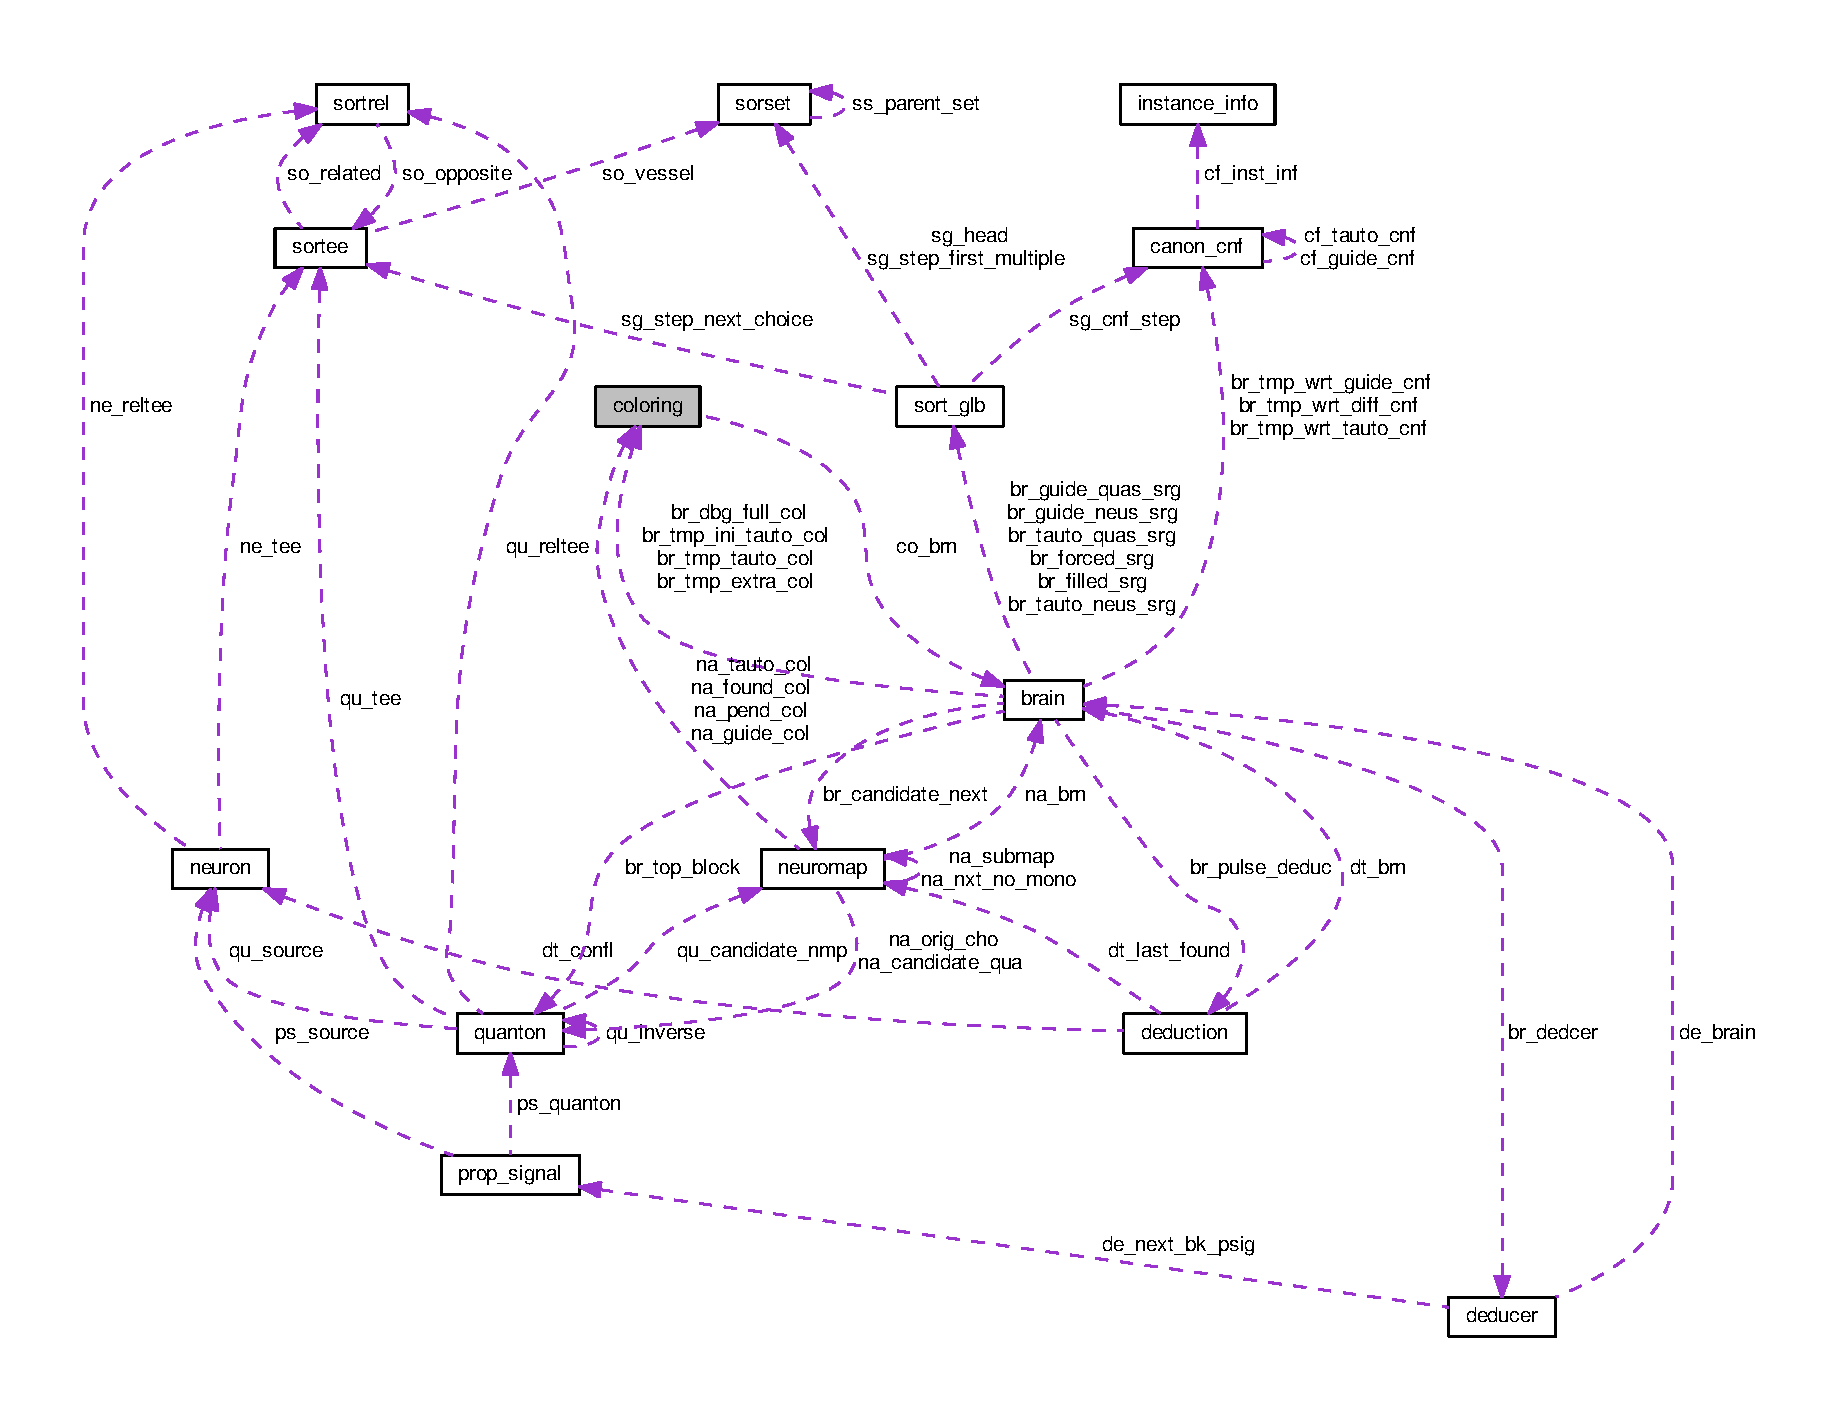
\includegraphics[width=350pt]{d0/d84/classcoloring__coll__graph}
\end{center}
\end{figure}


\subsection{Detailed Description}
The initial and final state for an stabilization is a coloring. 

A color is just an integer. A coloring of a sub-\/formula is an assignation of an integer (\hyperlink{classneuron}{neuron} -\/ color) to each \hyperlink{classneuron}{neuron} and an integer (\hyperlink{classquanton}{quanton} -\/color) to each \hyperlink{classquanton}{quanton} of the sub-\/formula. An stabilization may start with all neurons having the same neuron-\/color and all \hyperlink{classquanton}{quanton} s having the same \hyperlink{classquanton}{quanton} -\/color and finalize with each \hyperlink{classneuron}{neuron} having a unique \hyperlink{classneuron}{neuron} -\/ color and each \hyperlink{classquanton}{quanton} having a unique \hyperlink{classquanton}{quanton} -\/color, called a complete coloring.

colorings are ''loaded'' into the sortglb class in order to start stabilization. After stabilization the final coloring may be ''saved''. Each color in a coloring will correspond to one \hyperlink{classsorset}{sorset} during stabilization. These ''loading'' and ''saving'' words are used in the software only in relation to the sortglb class and have nothing to do with file operations.

This class is used to specify only the input to the stabilization process (the initial state). The class \hyperlink{classcanon__cnf}{canon\+\_\+cnf} is used for the output (it is the result of applying the output coloring (stabilized coloring) to the sub-\/formula it defines\+: \hyperlink{classneuron}{neuron} s and \hyperlink{classquanton}{quanton} s in the coloring. To initialize the sortor, it ''loads'' the initial coloring into the sortglb instance that will stabilize the C\+N\+F sub-\/formula. 

The documentation for this class was generated from the following files\+:\begin{DoxyCompactItemize}
\item 
/home/jose/devel/ben-\/jose/src/library/brain/\hyperlink{brain_8h}{brain.\+h}\item 
/home/jose/devel/ben-\/jose/src/library/brain/neuromap.\+cpp\item 
/home/jose/devel/ben-\/jose/src/library/debug/dbg\+\_\+brain.\+cpp\item 
/home/jose/devel/ben-\/jose/src/library/debug/dbg\+\_\+cy\+\_\+htm.\+cpp\end{DoxyCompactItemize}

\hypertarget{classdeducer}{}\section{deducer Class Reference}
\label{classdeducer}\index{deducer@{deducer}}


Class that holds the data used to analyze a conflict.  




{\ttfamily \#include $<$brain.\+h$>$}



Collaboration diagram for deducer\+:
% FIG 0
\subsection*{Public Member Functions}
\begin{DoxyCompactItemize}
\item 
void \hyperlink{classdeducer_a7db42a9dfc25ed6ed6747faea2c90961}{deduce} (\hyperlink{classdeduction}{deduction} \&dct, long max\+\_\+lv=I\+N\+V\+A\+L\+I\+D\+\_\+\+L\+E\+V\+EL)\hypertarget{classdeducer_a7db42a9dfc25ed6ed6747faea2c90961}{}\label{classdeducer_a7db42a9dfc25ed6ed6747faea2c90961}

\begin{DoxyCompactList}\small\item\em It does normal resolution analysis (C\+D\+CL). \end{DoxyCompactList}\end{DoxyCompactItemize}


\subsection{Detailed Description}
Class that holds the data used to analyze a conflict. 

The documentation for this class was generated from the following files\+:\begin{DoxyCompactItemize}
\item 
/home/jose/devel/ben-\/jose/src/library/brain/\hyperlink{brain_8h}{brain.\+h}\item 
/home/jose/devel/ben-\/jose/src/library/brain/deducer.\+cpp\item 
/home/jose/devel/ben-\/jose/src/library/debug/dbg\+\_\+brain.\+cpp\end{DoxyCompactItemize}

\hypertarget{classdeduction}{}\section{deduction Class Reference}
\label{classdeduction}\index{deduction@{deduction}}


Class that holds the result of analyzing (doing resolution) of a conflict.  




{\ttfamily \#include $<$brain.\+h$>$}



Collaboration diagram for deduction\+:
% FIG 0


\subsection{Detailed Description}
Class that holds the result of analyzing (doing resolution) of a conflict. 

It has the data for learning new \hyperlink{classneuron}{neuron} s (clauses). 

The documentation for this class was generated from the following files\+:\begin{DoxyCompactItemize}
\item 
/home/jose/devel/ben-\/jose/src/library/brain/\hyperlink{brain_8h}{brain.\+h}\item 
/home/jose/devel/ben-\/jose/src/library/brain/brain.\+cpp\item 
/home/jose/devel/ben-\/jose/src/library/brain/deducer.\+cpp\end{DoxyCompactItemize}

\hypertarget{classinstance__info}{\section{instance\+\_\+info Class Reference}
\label{classinstance__info}\index{instance\+\_\+info@{instance\+\_\+info}}
}


Class that holds an instance data.  




{\ttfamily \#include $<$instance\+\_\+info.\+h$>$}

\subsection*{Static Public Member Functions}
\begin{DoxyCompactItemize}
\item 
\hypertarget{classinstance__info_ac3abef1483f1c792526dae1b324bc7ee}{static void \hyperlink{classinstance__info_ac3abef1483f1c792526dae1b324bc7ee}{init\+\_\+output} (bj\+\_\+output\+\_\+t \&out)}\label{classinstance__info_ac3abef1483f1c792526dae1b324bc7ee}

\begin{DoxyCompactList}\small\item\em init and output \end{DoxyCompactList}\end{DoxyCompactItemize}


\subsection{Detailed Description}
Class that holds an instance data. 

The documentation for this class was generated from the following files\+:\begin{DoxyCompactItemize}
\item 
/home/jose/devel/ben-\/jose/src/library/brain/instance\+\_\+info.\+h\item 
/home/jose/devel/ben-\/jose/src/library/brain/brain.\+cpp\end{DoxyCompactItemize}

\hypertarget{classleveldat}{\section{leveldat Class Reference}
\label{classleveldat}\index{leveldat@{leveldat}}
}


Class that holds the data of a level.  




{\ttfamily \#include $<$brain.\+h$>$}



Collaboration diagram for leveldat\+:\nopagebreak
\begin{figure}[H]
\begin{center}
\leavevmode
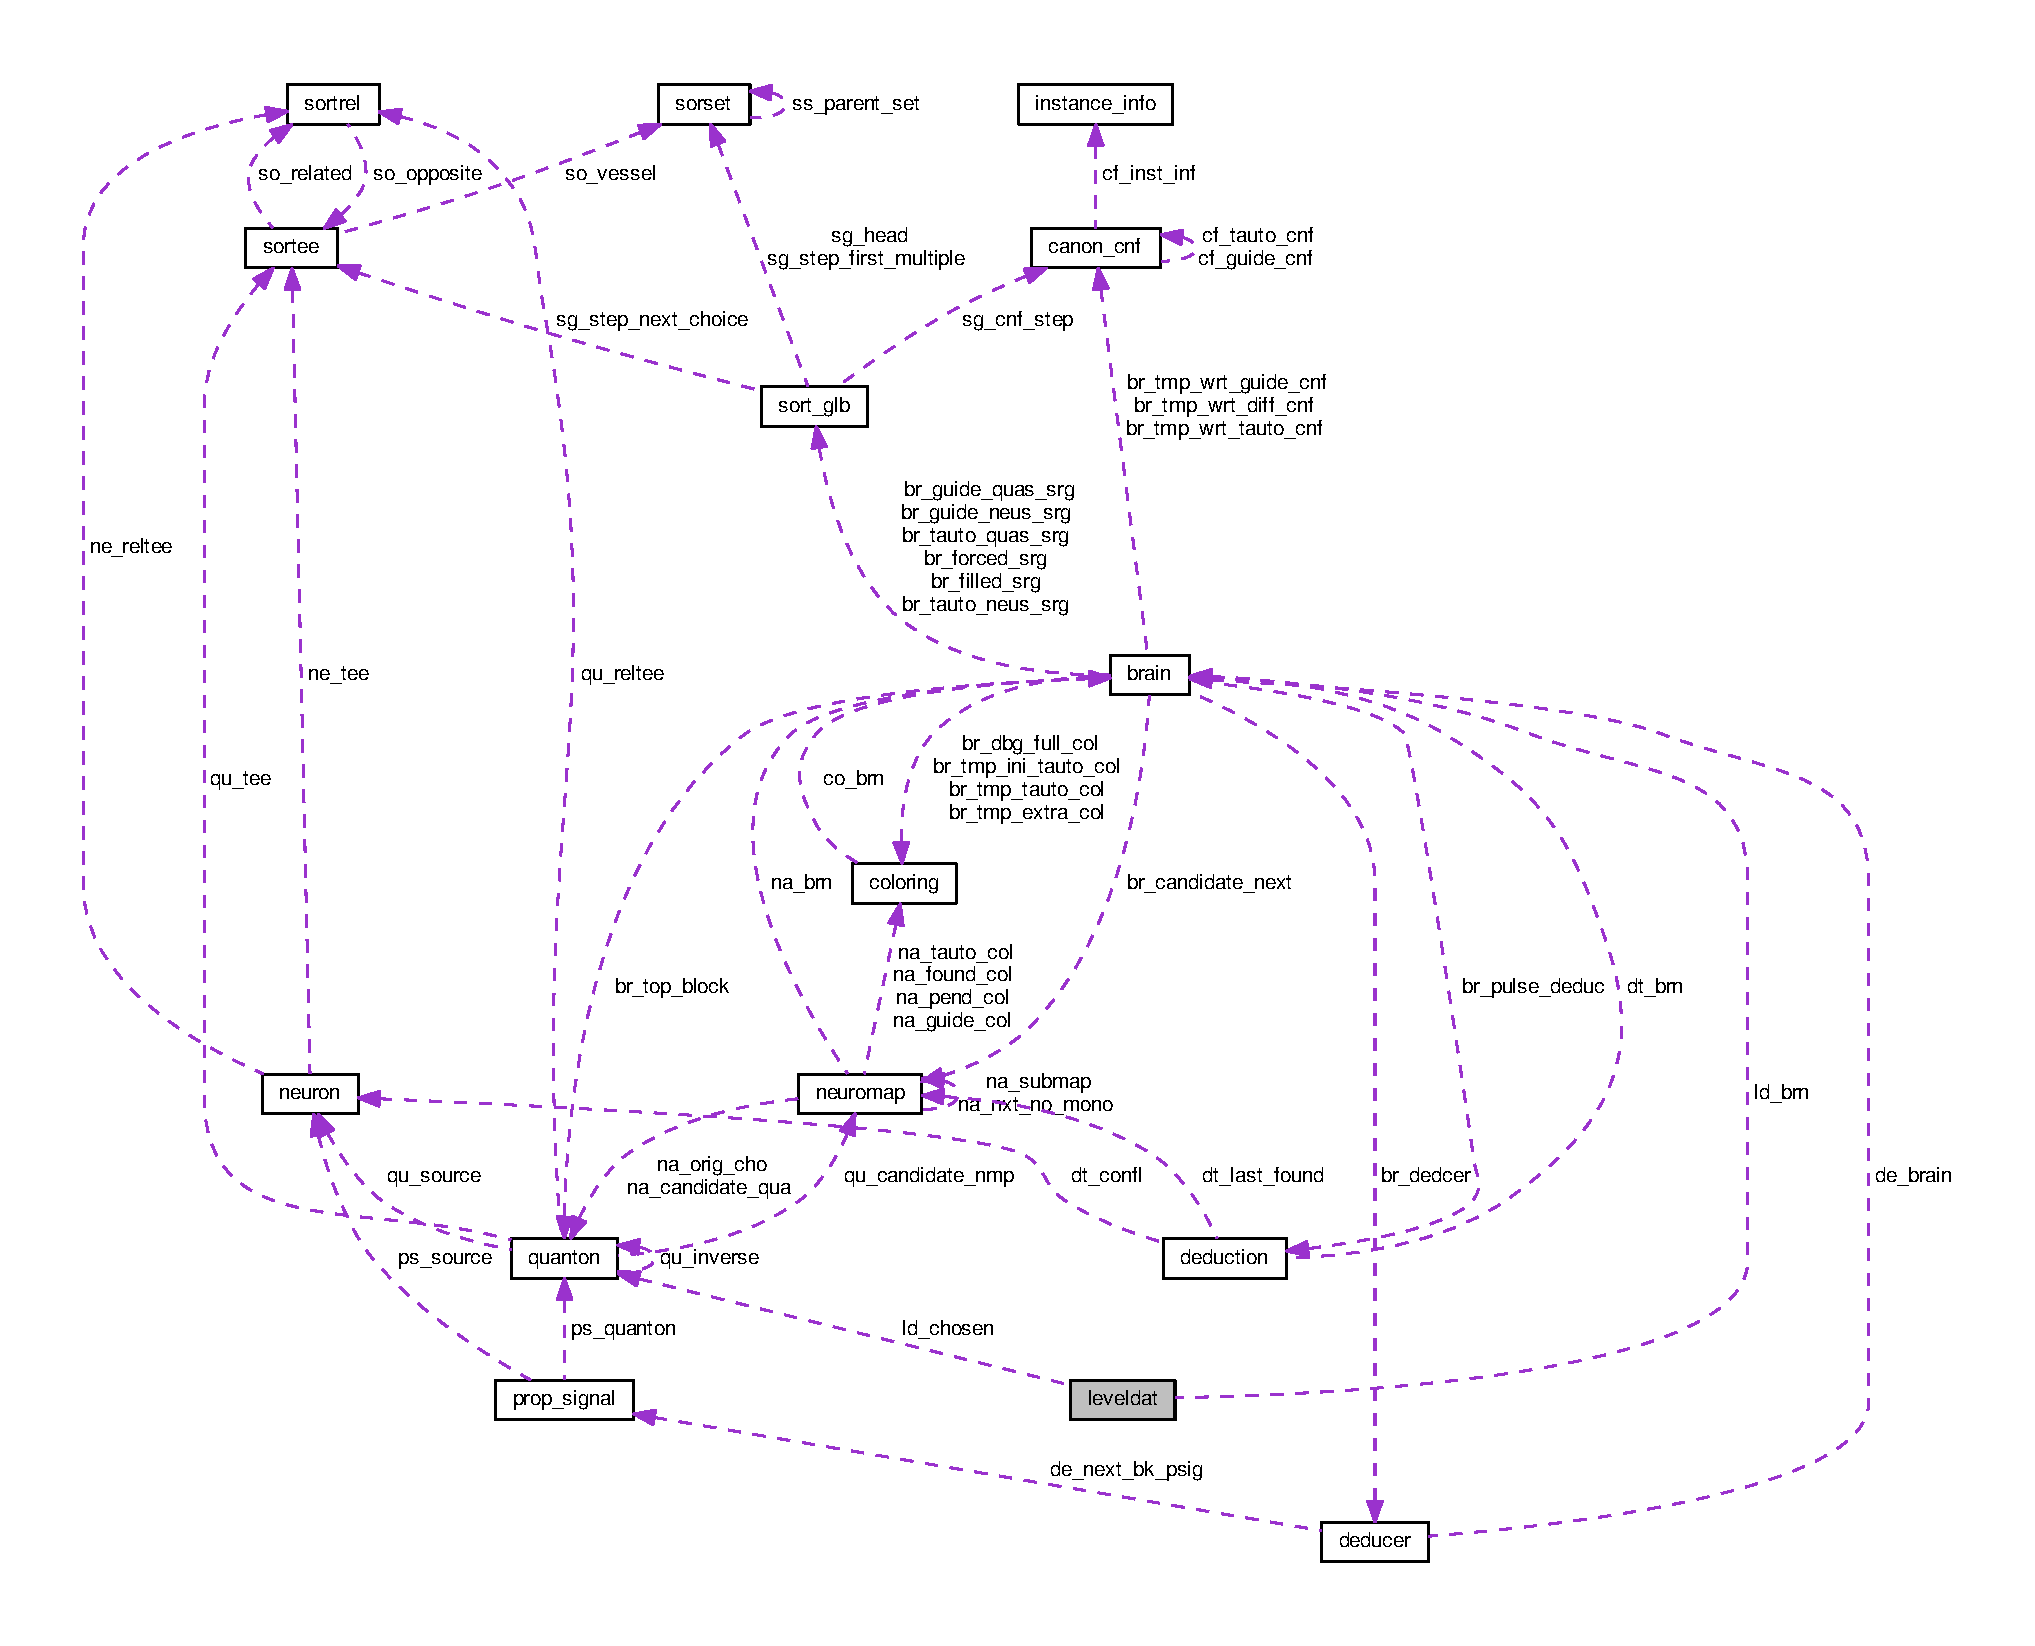
\includegraphics[width=350pt]{d1/de5/classleveldat__coll__graph}
\end{center}
\end{figure}


\subsection{Detailed Description}
Class that holds the data of a level. 

A level is all that happens between choices during B\+C\+P. So there is one level per choice. This class holds level relevant data. 

The documentation for this class was generated from the following files\+:\begin{DoxyCompactItemize}
\item 
/home/jose/devel/ben-\/jose/src/library/brain/\hyperlink{brain_8h}{brain.\+h}\item 
/home/jose/devel/ben-\/jose/src/library/brain/brain.\+cpp\item 
/home/jose/devel/ben-\/jose/src/library/debug/dbg\+\_\+brain.\+cpp\end{DoxyCompactItemize}

\hypertarget{classneuromap}{\section{neuromap Class Reference}
\label{classneuromap}\index{neuromap@{neuromap}}
}


A neuromap is a C\+N\+F sub-\/formula.  




{\ttfamily \#include $<$brain.\+h$>$}



Collaboration diagram for neuromap\+:\nopagebreak
\begin{figure}[H]
\begin{center}
\leavevmode
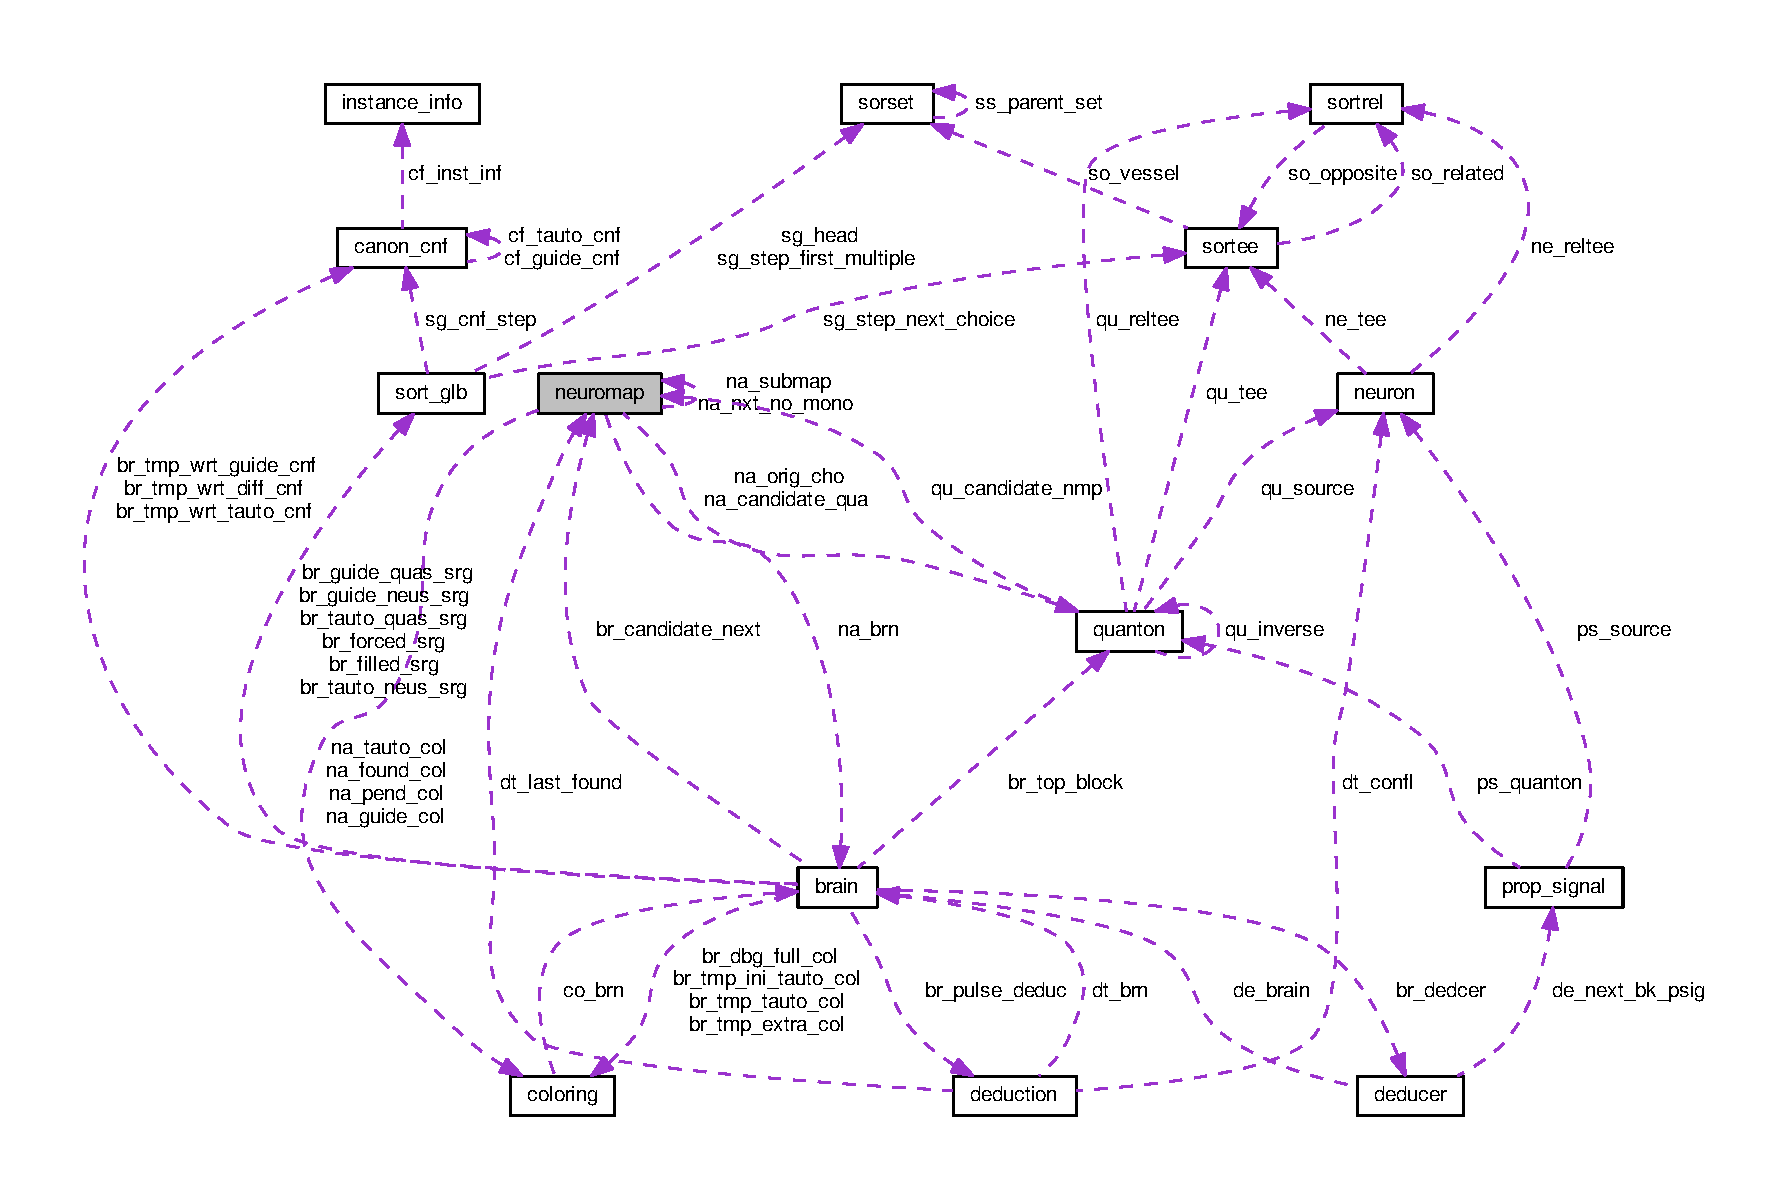
\includegraphics[width=350pt]{d2/d85/classneuromap__coll__graph}
\end{center}
\end{figure}
\subsection*{Public Member Functions}
\begin{DoxyCompactItemize}
\item 
bool \hyperlink{classneuromap_a5da738c0ecb7ba74a4fc435ca33b1fcb}{map\+\_\+find} ()
\begin{DoxyCompactList}\small\item\em It tries to find a \hyperlink{classneuromap}{neuromap}. \end{DoxyCompactList}\item 
bool \hyperlink{classneuromap_adb0c3a4698866c919272f9b4ba5998fd}{map\+\_\+write} (bool force\+\_\+full=false)
\begin{DoxyCompactList}\small\item\em It tries to write a \hyperlink{classneuromap}{neuromap}. \end{DoxyCompactList}\item 
bool \hyperlink{classneuromap_a5ad7c9c245129fc8a162742c11d4e972}{map\+\_\+oper} (mem\+\_\+op\+\_\+t mm)
\begin{DoxyCompactList}\small\item\em It stabilizes a \hyperlink{classneuromap}{neuromap} to a B\+C\+F\+F and then finds or writes the B\+C\+F\+F. \end{DoxyCompactList}\item 
bool \hyperlink{classneuromap_a9c0e877474e2d17cf8b9da564de8b8c3}{map\+\_\+prepare\+\_\+mem\+\_\+oper} (mem\+\_\+op\+\_\+t mm)
\begin{DoxyCompactList}\small\item\em It stabilizes a \hyperlink{classneuromap}{neuromap} to a B\+C\+F\+F. \end{DoxyCompactList}\end{DoxyCompactItemize}


\subsection{Detailed Description}
A neuromap is a C\+N\+F sub-\/formula. 

It is the pivot class to do all stabilization. It is maintained during B\+C\+P and used during backtracking in order to know what C\+N\+F sub-\/formulas are to be stabilized and searched for in the database (\hyperlink{classskeleton__glb}{skeleton\+\_\+glb} class). There is one neuromap per \hyperlink{classleveldat}{leveldat} and they are either active or inactive. Active when they are candidates for stabilizing, matching, searching and/or storing in the database, at backtrack time. During search, if a C\+N\+F sub-\/formula is found to be unsatisfiable, it is not trivial (too small), and both it's search branches had the same variables and clauses (so that it can latter be searched only with one of them), then the C\+N\+F sub-\/formula is stored in the database (\hyperlink{classskeleton__glb}{skeleton\+\_\+glb} class). Every time an still active neuromap has done its first branch of B\+C\+P, it is stabilized and searched for in the database (\hyperlink{classskeleton__glb}{skeleton\+\_\+glb} class). Trivial sub-\/formulas are basically ignored (see the use of 'brain\+::get\+\_\+min\+\_\+trainable\+\_\+num\+\_\+sub' method in the code). They are not searcned nor stored in \hyperlink{classskeleton__glb}{skeleton\+\_\+glb} (except for debugging purposes). 

\subsection{Member Function Documentation}
\hypertarget{classneuromap_a5da738c0ecb7ba74a4fc435ca33b1fcb}{\index{neuromap@{neuromap}!map\+\_\+find@{map\+\_\+find}}
\index{map\+\_\+find@{map\+\_\+find}!neuromap@{neuromap}}
\subsubsection[{map\+\_\+find}]{\setlength{\rightskip}{0pt plus 5cm}bool neuromap\+::map\+\_\+find (
\begin{DoxyParamCaption}
{}
\end{DoxyParamCaption}
)}}\label{classneuromap_a5da738c0ecb7ba74a4fc435ca33b1fcb}


It tries to find a \hyperlink{classneuromap}{neuromap}. 

\begin{DoxySeeAlso}{See also}
\hyperlink{macro__algorithm__ben__jose_8cpp}{macro\+\_\+algorithm\+\_\+ben\+\_\+jose.\+cpp} 
\end{DoxySeeAlso}


Here is the call graph for this function\+:\nopagebreak
\begin{figure}[H]
\begin{center}
\leavevmode
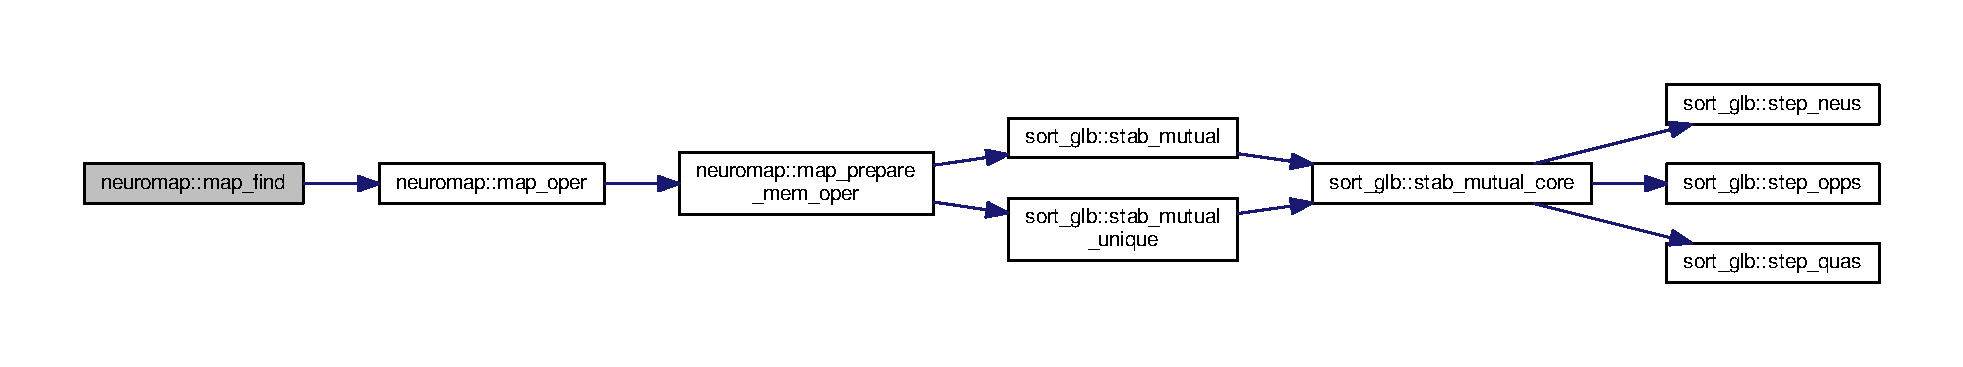
\includegraphics[width=350pt]{d6/d45/classneuromap_a5da738c0ecb7ba74a4fc435ca33b1fcb_cgraph}
\end{center}
\end{figure}




Here is the caller graph for this function\+:\nopagebreak
\begin{figure}[H]
\begin{center}
\leavevmode
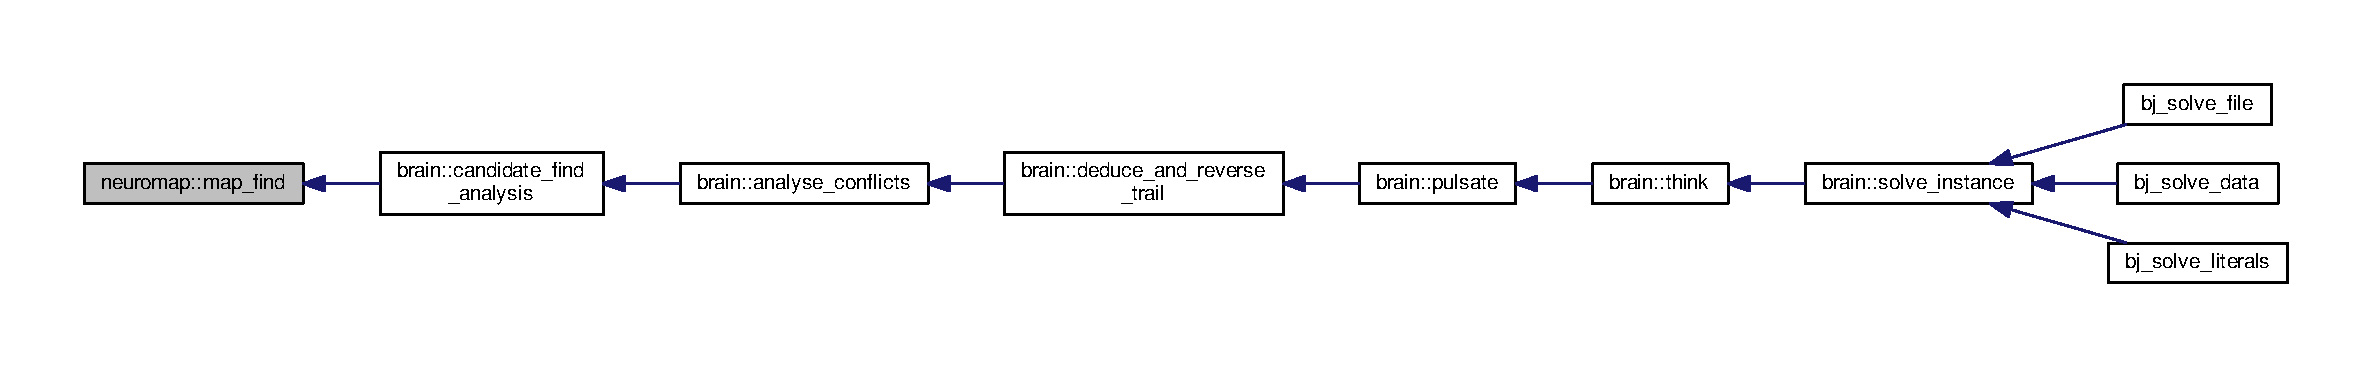
\includegraphics[width=350pt]{d6/d45/classneuromap_a5da738c0ecb7ba74a4fc435ca33b1fcb_icgraph}
\end{center}
\end{figure}


\hypertarget{classneuromap_adb0c3a4698866c919272f9b4ba5998fd}{\index{neuromap@{neuromap}!map\+\_\+write@{map\+\_\+write}}
\index{map\+\_\+write@{map\+\_\+write}!neuromap@{neuromap}}
\subsubsection[{map\+\_\+write}]{\setlength{\rightskip}{0pt plus 5cm}bool neuromap\+::map\+\_\+write (
\begin{DoxyParamCaption}
\item[{bool}]{force\+\_\+full = {\ttfamily false}}
\end{DoxyParamCaption}
)}}\label{classneuromap_adb0c3a4698866c919272f9b4ba5998fd}


It tries to write a \hyperlink{classneuromap}{neuromap}. 

\begin{DoxySeeAlso}{See also}
\hyperlink{macro__algorithm__ben__jose_8cpp}{macro\+\_\+algorithm\+\_\+ben\+\_\+jose.\+cpp} 
\end{DoxySeeAlso}


Here is the call graph for this function\+:\nopagebreak
\begin{figure}[H]
\begin{center}
\leavevmode
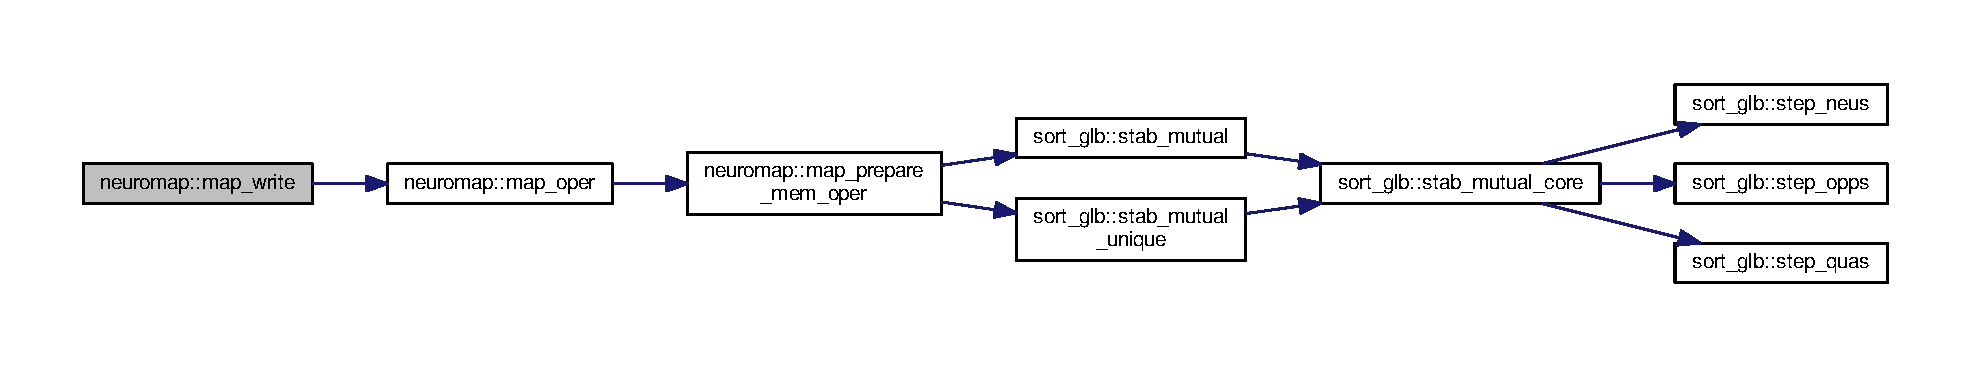
\includegraphics[width=350pt]{d6/d45/classneuromap_adb0c3a4698866c919272f9b4ba5998fd_cgraph}
\end{center}
\end{figure}




Here is the caller graph for this function\+:\nopagebreak
\begin{figure}[H]
\begin{center}
\leavevmode
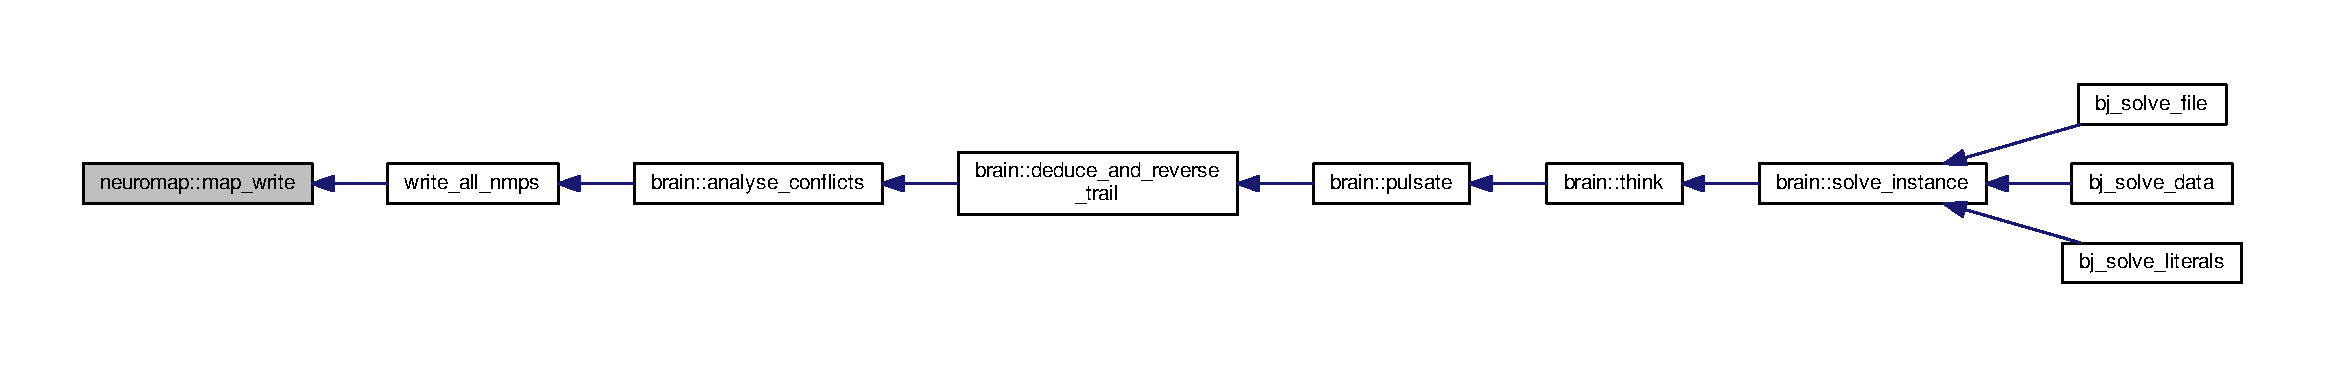
\includegraphics[width=350pt]{d6/d45/classneuromap_adb0c3a4698866c919272f9b4ba5998fd_icgraph}
\end{center}
\end{figure}


\hypertarget{classneuromap_a5ad7c9c245129fc8a162742c11d4e972}{\index{neuromap@{neuromap}!map\+\_\+oper@{map\+\_\+oper}}
\index{map\+\_\+oper@{map\+\_\+oper}!neuromap@{neuromap}}
\subsubsection[{map\+\_\+oper}]{\setlength{\rightskip}{0pt plus 5cm}bool neuromap\+::map\+\_\+oper (
\begin{DoxyParamCaption}
\item[{mem\+\_\+op\+\_\+t}]{mm}
\end{DoxyParamCaption}
)}}\label{classneuromap_a5ad7c9c245129fc8a162742c11d4e972}


It stabilizes a \hyperlink{classneuromap}{neuromap} to a B\+C\+F\+F and then finds or writes the B\+C\+F\+F. 

\begin{DoxySeeAlso}{See also}
\hyperlink{macro__algorithm__ben__jose_8cpp}{macro\+\_\+algorithm\+\_\+ben\+\_\+jose.\+cpp} 
\end{DoxySeeAlso}


Here is the call graph for this function\+:\nopagebreak
\begin{figure}[H]
\begin{center}
\leavevmode
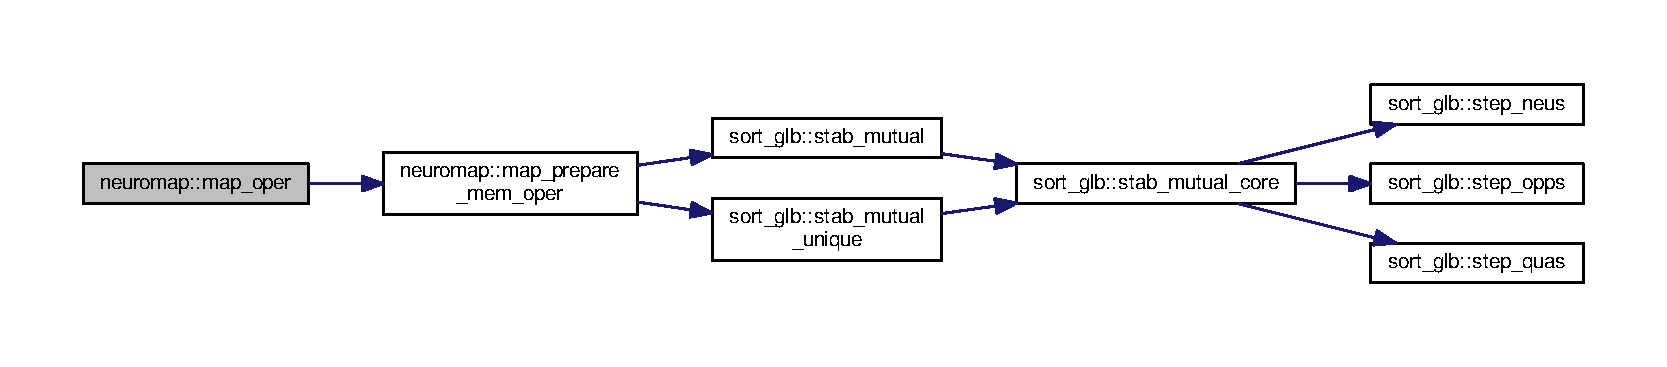
\includegraphics[width=350pt]{d6/d45/classneuromap_a5ad7c9c245129fc8a162742c11d4e972_cgraph}
\end{center}
\end{figure}




Here is the caller graph for this function\+:\nopagebreak
\begin{figure}[H]
\begin{center}
\leavevmode
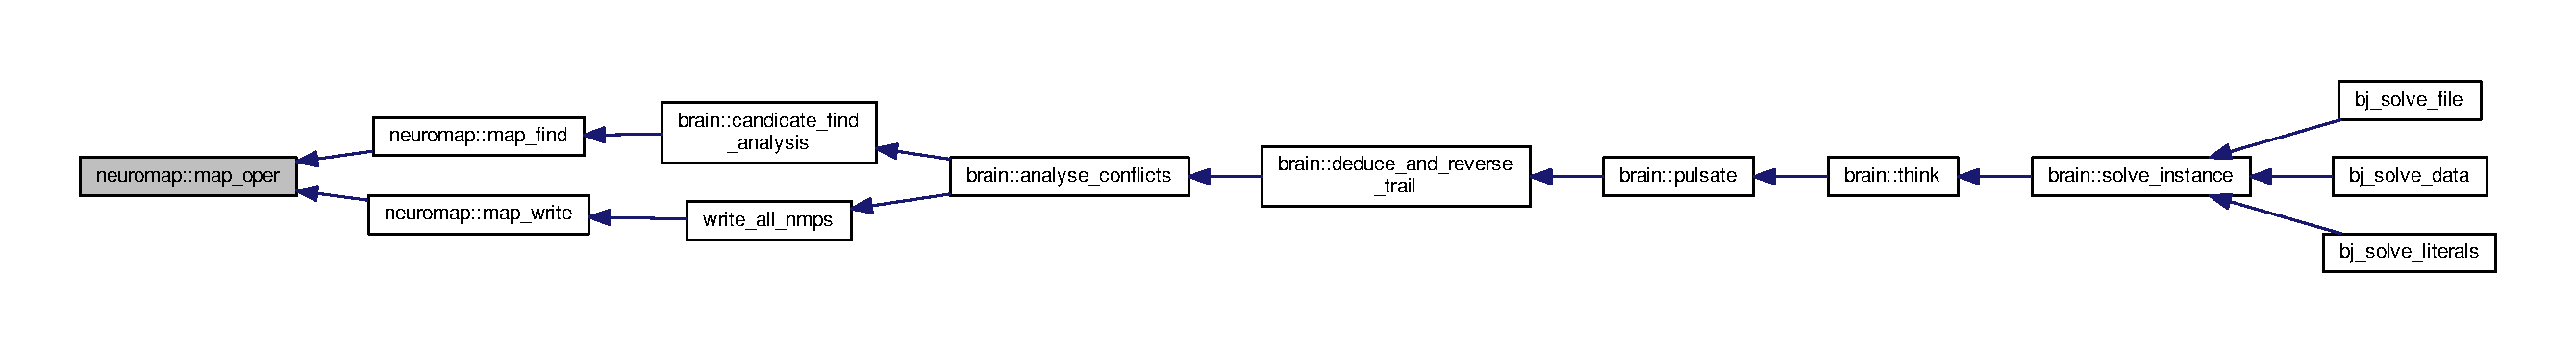
\includegraphics[width=350pt]{d6/d45/classneuromap_a5ad7c9c245129fc8a162742c11d4e972_icgraph}
\end{center}
\end{figure}


\hypertarget{classneuromap_a9c0e877474e2d17cf8b9da564de8b8c3}{\index{neuromap@{neuromap}!map\+\_\+prepare\+\_\+mem\+\_\+oper@{map\+\_\+prepare\+\_\+mem\+\_\+oper}}
\index{map\+\_\+prepare\+\_\+mem\+\_\+oper@{map\+\_\+prepare\+\_\+mem\+\_\+oper}!neuromap@{neuromap}}
\subsubsection[{map\+\_\+prepare\+\_\+mem\+\_\+oper}]{\setlength{\rightskip}{0pt plus 5cm}bool neuromap\+::map\+\_\+prepare\+\_\+mem\+\_\+oper (
\begin{DoxyParamCaption}
\item[{mem\+\_\+op\+\_\+t}]{mm}
\end{DoxyParamCaption}
)}}\label{classneuromap_a9c0e877474e2d17cf8b9da564de8b8c3}


It stabilizes a \hyperlink{classneuromap}{neuromap} to a B\+C\+F\+F. 

\begin{DoxySeeAlso}{See also}
\hyperlink{macro__algorithm__ben__jose_8cpp}{macro\+\_\+algorithm\+\_\+ben\+\_\+jose.\+cpp} 
\end{DoxySeeAlso}


Here is the call graph for this function\+:\nopagebreak
\begin{figure}[H]
\begin{center}
\leavevmode
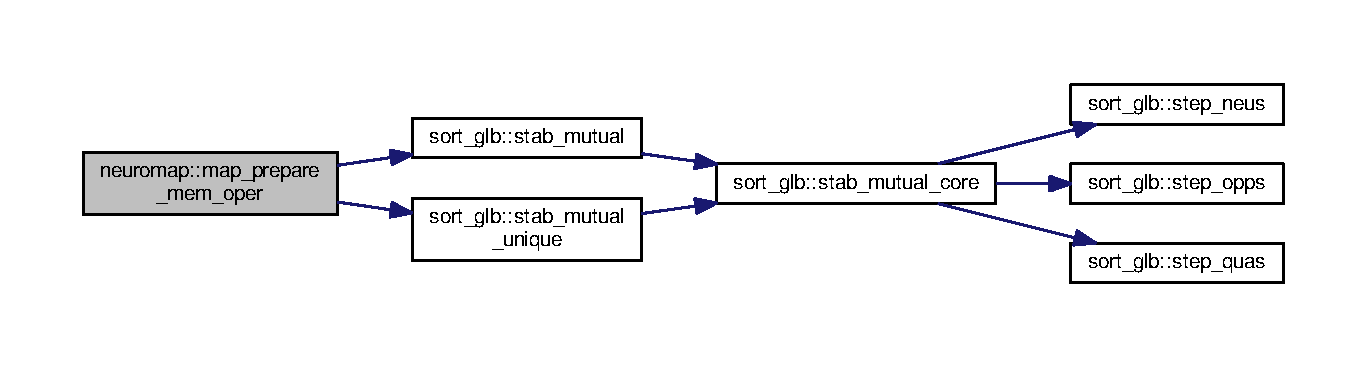
\includegraphics[width=350pt]{d6/d45/classneuromap_a9c0e877474e2d17cf8b9da564de8b8c3_cgraph}
\end{center}
\end{figure}




Here is the caller graph for this function\+:\nopagebreak
\begin{figure}[H]
\begin{center}
\leavevmode
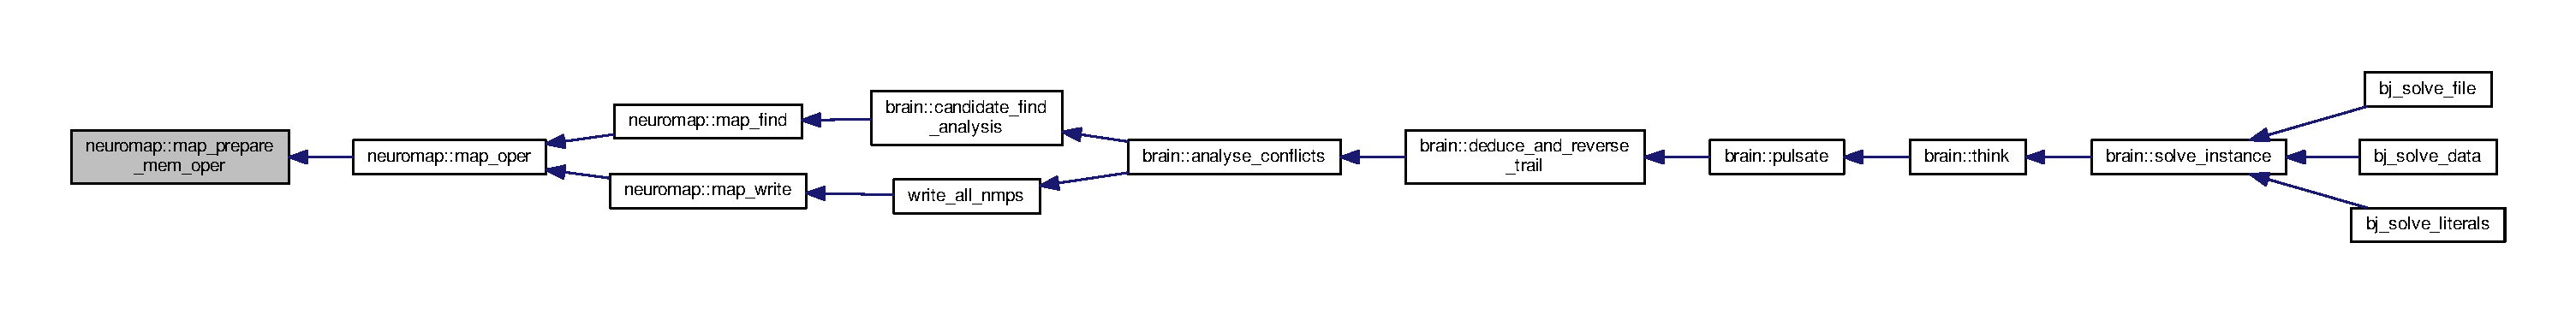
\includegraphics[width=350pt]{d6/d45/classneuromap_a9c0e877474e2d17cf8b9da564de8b8c3_icgraph}
\end{center}
\end{figure}




The documentation for this class was generated from the following files\+:\begin{DoxyCompactItemize}
\item 
/home/jose/devel/ben-\/jose/src/library/brain/\hyperlink{brain_8h}{brain.\+h}\item 
/home/jose/devel/ben-\/jose/src/library/api/macro\+\_\+ben\+\_\+jose.\+cpp\item 
/home/jose/devel/ben-\/jose/src/library/brain/brain.\+cpp\item 
/home/jose/devel/ben-\/jose/src/library/brain/deducer.\+cpp\item 
/home/jose/devel/ben-\/jose/src/library/brain/neuromap.\+cpp\item 
/home/jose/devel/ben-\/jose/src/library/debug/dbg\+\_\+brain.\+cpp\item 
/home/jose/devel/ben-\/jose/src/library/debug/dbg\+\_\+cy\+\_\+htm.\+cpp\item 
/home/jose/devel/ben-\/jose/src/programs/macro\+\_\+ben\+\_\+jose/\hyperlink{macro__algorithm__ben__jose_8cpp}{macro\+\_\+algorithm\+\_\+ben\+\_\+jose.\+cpp}\end{DoxyCompactItemize}

\hypertarget{classneuron}{}\section{neuron Class Reference}
\label{classneuron}\index{neuron@{neuron}}


Class for C\+NF clause behavior. So there is one neuron per clause.  




{\ttfamily \#include $<$brain.\+h$>$}



Collaboration diagram for neuron\+:
% FIG 0


\subsection{Detailed Description}
Class for C\+NF clause behavior. So there is one neuron per clause. 

The documentation for this class was generated from the following files\+:\begin{DoxyCompactItemize}
\item 
/home/jose/devel/ben-\/jose/src/library/brain/\hyperlink{brain_8h}{brain.\+h}\item 
/home/jose/devel/ben-\/jose/src/library/brain/brain.\+cpp\item 
/home/jose/devel/ben-\/jose/src/library/brain/deducer.\+cpp\item 
/home/jose/devel/ben-\/jose/src/library/brain/neuromap.\+cpp\item 
/home/jose/devel/ben-\/jose/src/library/debug/dbg\+\_\+brain.\+cpp\item 
/home/jose/devel/ben-\/jose/src/library/debug/dbg\+\_\+cy\+\_\+htm.\+cpp\end{DoxyCompactItemize}

\hypertarget{classprop__signal}{}\section{prop\+\_\+signal Class Reference}
\label{classprop__signal}\index{prop\+\_\+signal@{prop\+\_\+signal}}


Class for representing B\+CP propagation data.  




{\ttfamily \#include $<$brain.\+h$>$}



Collaboration diagram for prop\+\_\+signal\+:
% FIG 0


\subsection{Detailed Description}
Class for representing B\+CP propagation data. 

Which \hyperlink{classquanton}{quanton} fired by which \hyperlink{classneuron}{neuron} (which clause forced a given variable). B\+CP is done with the two watched literals technique (two watched fibres in the library\textquotesingle{}s terminology). 

The documentation for this class was generated from the following files\+:\begin{DoxyCompactItemize}
\item 
/home/jose/devel/ben-\/jose/src/library/brain/\hyperlink{brain_8h}{brain.\+h}\item 
/home/jose/devel/ben-\/jose/src/library/brain/deducer.\+cpp\item 
/home/jose/devel/ben-\/jose/src/library/debug/dbg\+\_\+brain.\+cpp\end{DoxyCompactItemize}

\hypertarget{classquanton}{\section{quanton Class Reference}
\label{classquanton}\index{quanton@{quanton}}
}


Class for C\+N\+F variables (each variable has a positon and a negaton).  




{\ttfamily \#include $<$brain.\+h$>$}



Collaboration diagram for quanton\+:\nopagebreak
\begin{figure}[H]
\begin{center}
\leavevmode
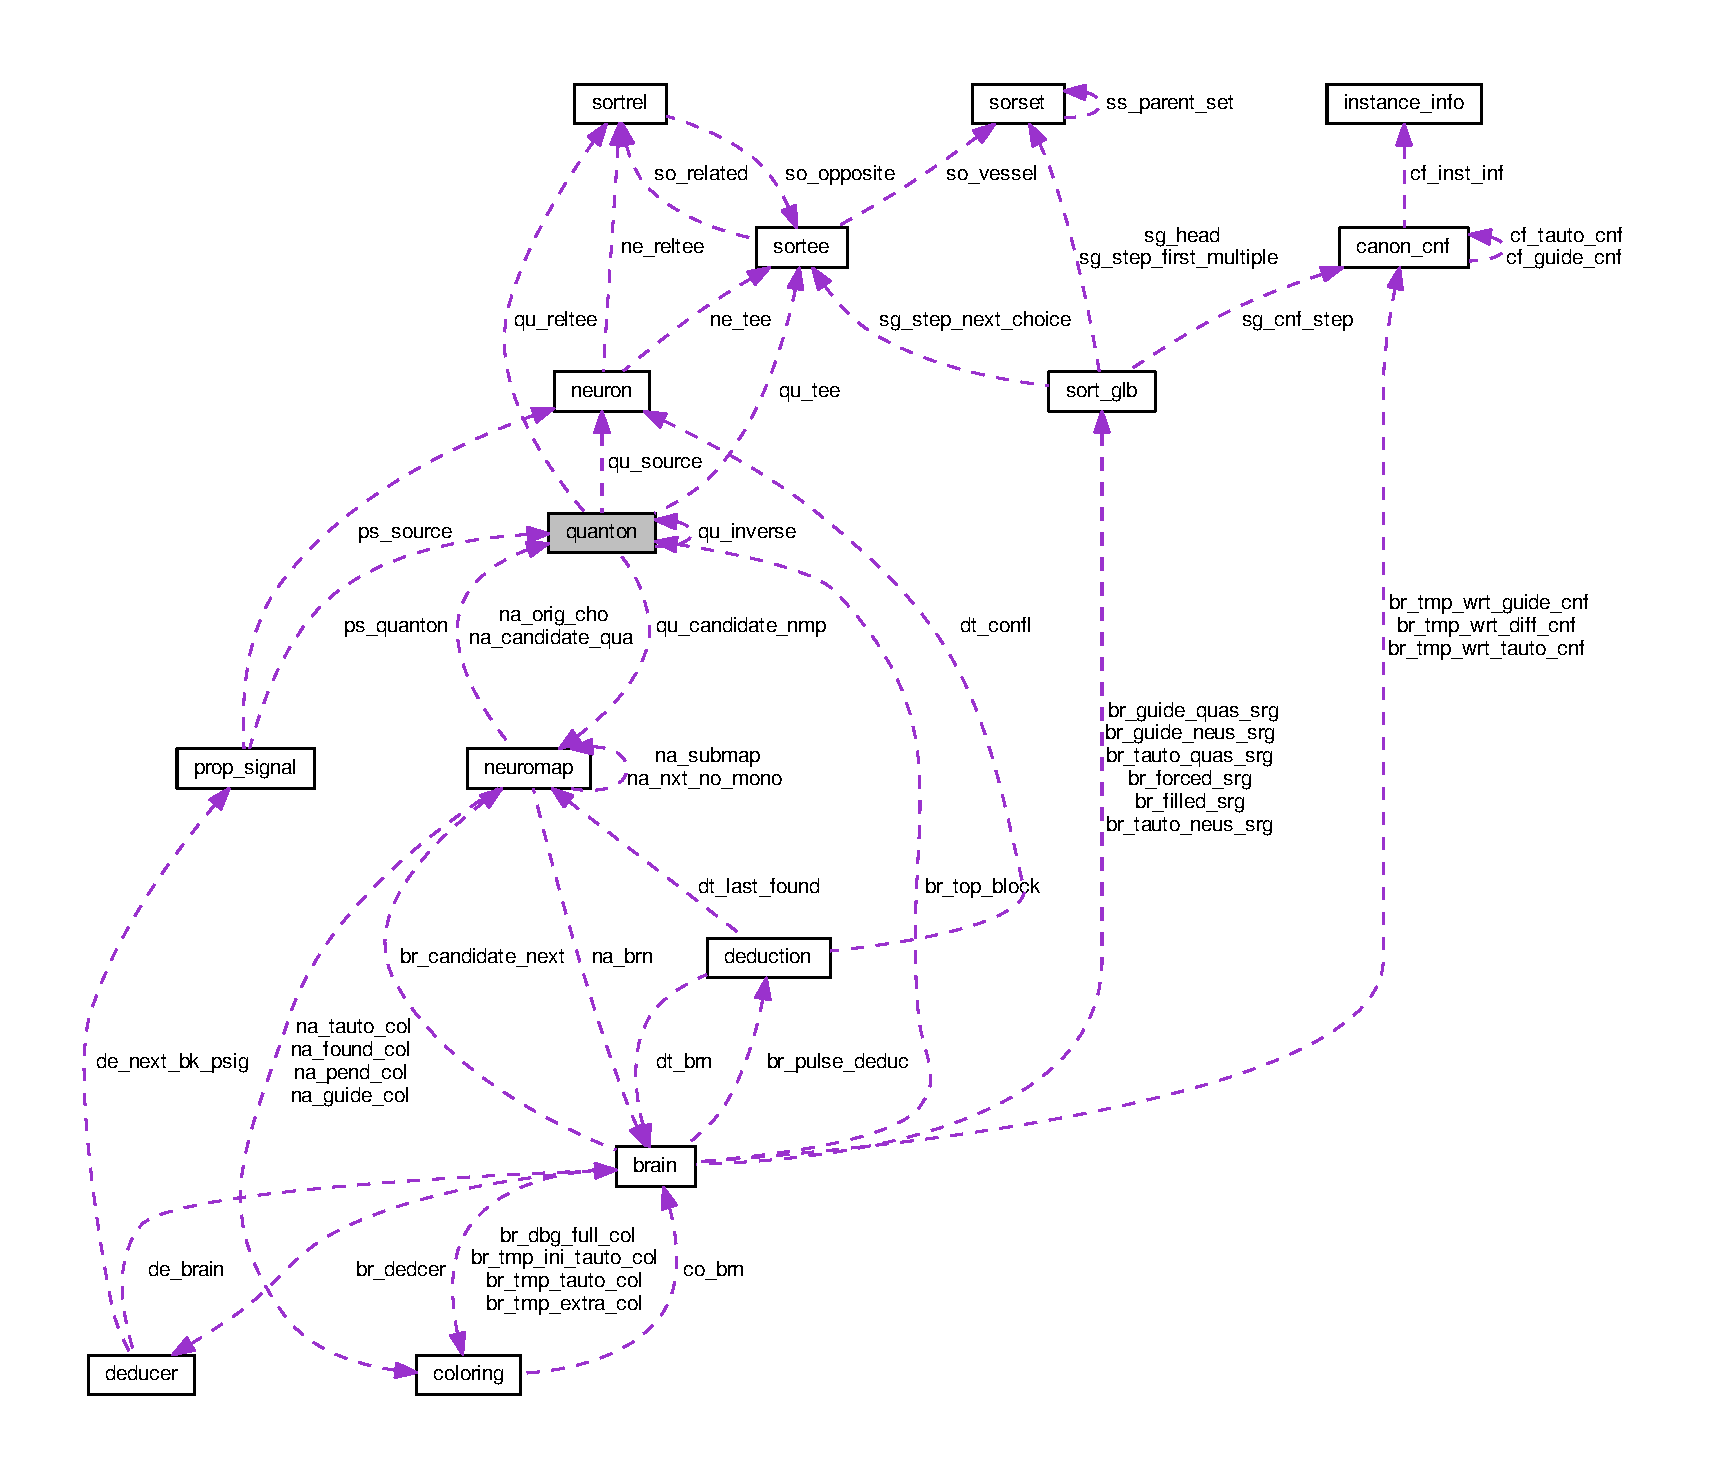
\includegraphics[width=350pt]{df/d7b/classquanton__coll__graph}
\end{center}
\end{figure}


\subsection{Detailed Description}
Class for C\+N\+F variables (each variable has a positon and a negaton). 

There are two \hyperlink{classquanton}{quanton} s per variable. \hyperlink{classneuron}{neuron} s hold references to \hyperlink{classquanton}{quanton} s called fibres. They are used for B\+C\+P. 

The documentation for this class was generated from the following files\+:\begin{DoxyCompactItemize}
\item 
/home/jose/devel/ben-\/jose/src/library/brain/\hyperlink{brain_8h}{brain.\+h}\item 
/home/jose/devel/ben-\/jose/src/library/brain/brain.\+cpp\item 
/home/jose/devel/ben-\/jose/src/library/brain/deducer.\+cpp\item 
/home/jose/devel/ben-\/jose/src/library/brain/neuromap.\+cpp\item 
/home/jose/devel/ben-\/jose/src/library/debug/dbg\+\_\+brain.\+cpp\item 
/home/jose/devel/ben-\/jose/src/library/debug/dbg\+\_\+cy\+\_\+htm.\+cpp\end{DoxyCompactItemize}

\hypertarget{structsha2__context}{\section{sha2\+\_\+context Struct Reference}
\label{structsha2__context}\index{sha2\+\_\+context@{sha2\+\_\+context}}
}


S\+H\+A-\/256 context structure.  




{\ttfamily \#include $<$sha2.\+h$>$}

\subsection*{Public Attributes}
\begin{DoxyCompactItemize}
\item 
unsigned long \hyperlink{structsha2__context_a485843c955ab26a3d78d499934371df1}{total} \mbox{[}2\mbox{]}
\item 
unsigned long \hyperlink{structsha2__context_a61a62a66ac1851bcd90aa65e7fad1328}{state} \mbox{[}8\mbox{]}
\item 
unsigned char \hyperlink{structsha2__context_aa5c93c2e2e8fc23008a849ea4f9a0b91}{buffer} \mbox{[}64\mbox{]}
\item 
unsigned char \hyperlink{structsha2__context_a4b003f9de8a8d823d19e813311764bd2}{ipad} \mbox{[}64\mbox{]}
\item 
unsigned char \hyperlink{structsha2__context_a3f710fbbb4c2c1ce3d57de40b1036cea}{opad} \mbox{[}64\mbox{]}
\item 
int \hyperlink{structsha2__context_a20fd61f8c14d811e93b7186ca71ecfbd}{is224}
\end{DoxyCompactItemize}


\subsection{Detailed Description}
S\+H\+A-\/256 context structure. 

\subsection{Member Data Documentation}
\hypertarget{structsha2__context_a485843c955ab26a3d78d499934371df1}{\index{sha2\+\_\+context@{sha2\+\_\+context}!total@{total}}
\index{total@{total}!sha2\+\_\+context@{sha2\+\_\+context}}
\subsubsection[{total}]{\setlength{\rightskip}{0pt plus 5cm}unsigned long sha2\+\_\+context\+::total\mbox{[}2\mbox{]}}}\label{structsha2__context_a485843c955ab26a3d78d499934371df1}
number of bytes processed \hypertarget{structsha2__context_a61a62a66ac1851bcd90aa65e7fad1328}{\index{sha2\+\_\+context@{sha2\+\_\+context}!state@{state}}
\index{state@{state}!sha2\+\_\+context@{sha2\+\_\+context}}
\subsubsection[{state}]{\setlength{\rightskip}{0pt plus 5cm}unsigned long sha2\+\_\+context\+::state\mbox{[}8\mbox{]}}}\label{structsha2__context_a61a62a66ac1851bcd90aa65e7fad1328}
intermediate digest state \hypertarget{structsha2__context_aa5c93c2e2e8fc23008a849ea4f9a0b91}{\index{sha2\+\_\+context@{sha2\+\_\+context}!buffer@{buffer}}
\index{buffer@{buffer}!sha2\+\_\+context@{sha2\+\_\+context}}
\subsubsection[{buffer}]{\setlength{\rightskip}{0pt plus 5cm}unsigned char sha2\+\_\+context\+::buffer\mbox{[}64\mbox{]}}}\label{structsha2__context_aa5c93c2e2e8fc23008a849ea4f9a0b91}
data block being processed \hypertarget{structsha2__context_a4b003f9de8a8d823d19e813311764bd2}{\index{sha2\+\_\+context@{sha2\+\_\+context}!ipad@{ipad}}
\index{ipad@{ipad}!sha2\+\_\+context@{sha2\+\_\+context}}
\subsubsection[{ipad}]{\setlength{\rightskip}{0pt plus 5cm}unsigned char sha2\+\_\+context\+::ipad\mbox{[}64\mbox{]}}}\label{structsha2__context_a4b003f9de8a8d823d19e813311764bd2}
H\+M\+A\+C\+: inner padding \hypertarget{structsha2__context_a3f710fbbb4c2c1ce3d57de40b1036cea}{\index{sha2\+\_\+context@{sha2\+\_\+context}!opad@{opad}}
\index{opad@{opad}!sha2\+\_\+context@{sha2\+\_\+context}}
\subsubsection[{opad}]{\setlength{\rightskip}{0pt plus 5cm}unsigned char sha2\+\_\+context\+::opad\mbox{[}64\mbox{]}}}\label{structsha2__context_a3f710fbbb4c2c1ce3d57de40b1036cea}
H\+M\+A\+C\+: outer padding \hypertarget{structsha2__context_a20fd61f8c14d811e93b7186ca71ecfbd}{\index{sha2\+\_\+context@{sha2\+\_\+context}!is224@{is224}}
\index{is224@{is224}!sha2\+\_\+context@{sha2\+\_\+context}}
\subsubsection[{is224}]{\setlength{\rightskip}{0pt plus 5cm}int sha2\+\_\+context\+::is224}}\label{structsha2__context_a20fd61f8c14d811e93b7186ca71ecfbd}
0 if S\+H\+A-\/256, 1 if S\+H\+A-\/224 

The documentation for this struct was generated from the following file\+:\begin{DoxyCompactItemize}
\item 
/home/jose/devel/ben-\/jose/src/utils/\hyperlink{sha2_8h}{sha2.\+h}\end{DoxyCompactItemize}

\hypertarget{classskeleton__glb}{}\section{skeleton\+\_\+glb Class Reference}
\label{classskeleton__glb}\index{skeleton\+\_\+glb@{skeleton\+\_\+glb}}


A \hyperlink{classskeleton__glb}{skeleton\+\_\+glb} is a directory holding a database.  




{\ttfamily \#include $<$skeleton.\+h$>$}



Collaboration diagram for skeleton\+\_\+glb\+:
% FIG 0


\subsection{Detailed Description}
A \hyperlink{classskeleton__glb}{skeleton\+\_\+glb} is a directory holding a database. 

The skeleton class handles all disk related functions and management. The database is basically a directory and all its sub-\/directories in disk. The directory (skeleton) is seen as a group of (\textquotesingle{}\textquotesingle{}key\textquotesingle{}\textquotesingle{},\textquotesingle{}\textquotesingle{}value\textquotesingle{}\textquotesingle{}) pairs. Just like a common database \textquotesingle{}\textquotesingle{}index\textquotesingle{}\textquotesingle{}, a \textquotesingle{}\textquotesingle{}dictionary\textquotesingle{}\textquotesingle{} class, or a \textquotesingle{}\textquotesingle{}map\textquotesingle{}\textquotesingle{} class. A path within the skeleton is a \textquotesingle{}\textquotesingle{}key\textquotesingle{}\textquotesingle{} and the files in the path are the \textquotesingle{}\textquotesingle{}value\textquotesingle{}\textquotesingle{}. To see if a \textquotesingle{}\textquotesingle{}key\textquotesingle{}\textquotesingle{} exists is to see if a path exists within the skeleton. Unsatisfiable canoncnf s are saved and searched by the S\+HA function of their content. They are saved in a path (\textquotesingle{}\textquotesingle{}key\textquotesingle{}\textquotesingle{}) that is constructed with the S\+HA and other relevant search info.

Since an unsatisfiable sub-\/formula might not be minimal (have some unnecessary clauses for unsatisfiability), each unsatisfiable C\+NF sub-\/formula has three relevant canoncnf \+:


\begin{DoxyItemize}
\item The guide. It is the canoncnf resulting of stabilizing the C\+NF sub-\/formula covered by first search branch variables. So it is a satisfiable part of the unsatisfiable C\+NF sub-\/formula that is a \textquotesingle{}\textquotesingle{}guide\textquotesingle{}\textquotesingle{} for the search.


\item The tauto. It is the full unsatisfiable C\+NF sub-\/formula. It is the canoncnf resulting of stabilizing the C\+NF sub-\/formula covered by both search branches charged \hyperlink{classquanton}{quanton} s (used variables).


\item The diff. This canoncnf contains all canon\+\_\+clause s in tauto but not in guide. Each diff is saved in a path called \textquotesingle{}variant\textquotesingle{} in the skeleton. So one guide can have several variants. 
\end{DoxyItemize}

A search of a target C\+NF sub-\/formula is conducted in two phases\+: the search for the guide of the target and the search for the variant that is a sub-\/formula of the target diff. Once the guide is stabilized the search for it is a simple\+: \textquotesingle{}\textquotesingle{}see if its path exists\textquotesingle{}\textquotesingle{} (remember that its path contains the S\+HA of its content). If the target canoncnf is not equal to a variant (the path does not exist), the second phase is more time consuming because it involves reading each variant and comparing it to the target diff to see if the the variant is a sub-\/formula of the target diff (which would mean that the target is unsatisfiable and therefore can be backtracked). 

The documentation for this class was generated from the following files\+:\begin{DoxyCompactItemize}
\item 
/home/jose/devel/ben-\/jose/src/library/unsat\+\_\+db/skeleton.\+h\item 
/home/jose/devel/ben-\/jose/src/library/unsat\+\_\+db/skeleton.\+cpp\end{DoxyCompactItemize}

\hypertarget{classsorset}{\section{sorset Class Reference}
\label{classsorset}\index{sorset@{sorset}}
}


A sorset is a group of \hyperlink{classsortee}{sortee} s.  




{\ttfamily \#include $<$sortor.\+h$>$}



Collaboration diagram for sorset\+:\nopagebreak
\begin{figure}[H]
\begin{center}
\leavevmode
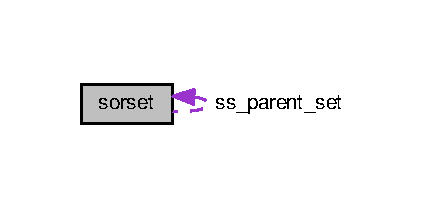
\includegraphics[width=206pt]{d0/d4c/classsorset__coll__graph}
\end{center}
\end{figure}
\subsection*{Public Member Functions}
\begin{DoxyCompactItemize}
\item 
void \hyperlink{classsorset_a9a85b9412bc1fc5bea86d416e52b55c7}{step\+\_\+mutual\+\_\+stabilize\+\_\+rec} (\hyperlink{classsort__glb}{sort\+\_\+glb} \&srg1, \hyperlink{classsort__glb}{sort\+\_\+glb} \&srg2)
\begin{DoxyCompactList}\small\item\em It does \hyperlink{classsortee_a5cc113e22e62dfcb3869c2786ae5345e}{sortee\+::sort\+\_\+from} operations on this \hyperlink{classsorset}{sorset} 's \hyperlink{classsortee}{sortee} s. \end{DoxyCompactList}\end{DoxyCompactItemize}


\subsection{Detailed Description}
A sorset is a group of \hyperlink{classsortee}{sortee} s. 

In order to stabilize a group of \hyperlink{classsortee}{sortee} s the \hyperlink{classsort__glb}{sort\+\_\+glb} class (or sortor) groups \hyperlink{classsortee}{sortee} s (representing \hyperlink{classneuron}{neuron} s and \hyperlink{classquanton}{quanton} s in our case) into \hyperlink{classsorset}{sorset} s. A sub-\/formula is represented within stabilization by a group of \hyperlink{classsorset}{sorset} s. Each step of stabilization refines the group of \hyperlink{classsorset}{sorset} s that represent the stabilizing sub-\/formula, so that every step there are more \hyperlink{classsorset}{sorset} s, each one having less \hyperlink{classsortee}{sortee} s, until the process cannot refine each \hyperlink{classsorset}{sorset} anymore. The ideal stabilization ends with each \hyperlink{classsorset}{sorset} containing only one \hyperlink{classsortee}{sortee}. Since stabilization handles only \hyperlink{classsortee}{sortee} s. This class is used for such iterated sub-\/grouping. 

\subsection{Member Function Documentation}
\hypertarget{classsorset_a9a85b9412bc1fc5bea86d416e52b55c7}{\index{sorset@{sorset}!step\+\_\+mutual\+\_\+stabilize\+\_\+rec@{step\+\_\+mutual\+\_\+stabilize\+\_\+rec}}
\index{step\+\_\+mutual\+\_\+stabilize\+\_\+rec@{step\+\_\+mutual\+\_\+stabilize\+\_\+rec}!sorset@{sorset}}
\subsubsection[{step\+\_\+mutual\+\_\+stabilize\+\_\+rec}]{\setlength{\rightskip}{0pt plus 5cm}void sorset\+::step\+\_\+mutual\+\_\+stabilize\+\_\+rec (
\begin{DoxyParamCaption}
\item[{{\bf sort\+\_\+glb} \&}]{srg1, }
\item[{{\bf sort\+\_\+glb} \&}]{srg2}
\end{DoxyParamCaption}
)}}\label{classsorset_a9a85b9412bc1fc5bea86d416e52b55c7}


It does \hyperlink{classsortee_a5cc113e22e62dfcb3869c2786ae5345e}{sortee\+::sort\+\_\+from} operations on this \hyperlink{classsorset}{sorset} 's \hyperlink{classsortee}{sortee} s. 


\begin{DoxyParams}{Parameters}
{\em srg1} & The base sort\+\_\+glb\+:
\begin{DoxyItemize}
\item A \hyperlink{classneuron}{neuron} s \hyperlink{classsort__glb}{sort\+\_\+glb} if stabilizing \hyperlink{classneuron}{neuron} \hyperlink{classsortee}{sortee} s
\item A \hyperlink{classquanton}{quanton} s \hyperlink{classsort__glb}{sort\+\_\+glb} if stabilizing \hyperlink{classquanton}{quanton} \hyperlink{classsortee}{sortee} s 
\end{DoxyItemize}\\
\hline
{\em srg2} & The complement of srg1\+:
\begin{DoxyItemize}
\item A \hyperlink{classquanton}{quanton} s \hyperlink{classsort__glb}{sort\+\_\+glb} if srg1 is a \hyperlink{classneuron}{neuron} s \hyperlink{classsort__glb}{sort\+\_\+glb}
\item A \hyperlink{classneuron}{neuron} s \hyperlink{classsort__glb}{sort\+\_\+glb} if srg1 is a \hyperlink{classquanton}{quanton} s \hyperlink{classsort__glb}{sort\+\_\+glb} 
\end{DoxyItemize}\\
\hline
\end{DoxyParams}
\begin{DoxySeeAlso}{See also}
\hyperlink{macro__algorithm__ben__jose_8cpp}{macro\+\_\+algorithm\+\_\+ben\+\_\+jose.\+cpp} 
\end{DoxySeeAlso}


Here is the call graph for this function\+:\nopagebreak
\begin{figure}[H]
\begin{center}
\leavevmode
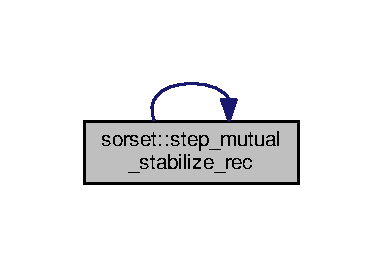
\includegraphics[width=184pt]{d3/d62/classsorset_a9a85b9412bc1fc5bea86d416e52b55c7_cgraph}
\end{center}
\end{figure}




Here is the caller graph for this function\+:\nopagebreak
\begin{figure}[H]
\begin{center}
\leavevmode
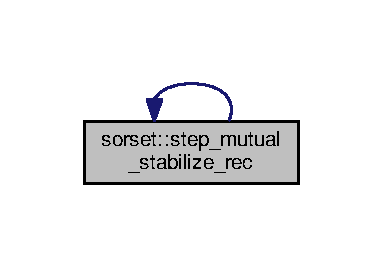
\includegraphics[width=184pt]{d3/d62/classsorset_a9a85b9412bc1fc5bea86d416e52b55c7_icgraph}
\end{center}
\end{figure}




The documentation for this class was generated from the following files\+:\begin{DoxyCompactItemize}
\item 
/home/jose/devel/ben-\/jose/src/library/brain/sortor.\+h\item 
/home/jose/devel/ben-\/jose/src/library/api/macro\+\_\+ben\+\_\+jose.\+cpp\item 
/home/jose/devel/ben-\/jose/src/library/brain/sortor.\+cpp\item 
/home/jose/devel/ben-\/jose/src/programs/macro\+\_\+ben\+\_\+jose/\hyperlink{macro__algorithm__ben__jose_8cpp}{macro\+\_\+algorithm\+\_\+ben\+\_\+jose.\+cpp}\end{DoxyCompactItemize}

\hypertarget{classsort__glb}{\section{sort\+\_\+glb Class Reference}
\label{classsort__glb}\index{sort\+\_\+glb@{sort\+\_\+glb}}
}


Class that holds all global data used to stabilize a group of items.  




{\ttfamily \#include $<$sortor.\+h$>$}



Collaboration diagram for sort\+\_\+glb\+:\nopagebreak
\begin{figure}[H]
\begin{center}
\leavevmode
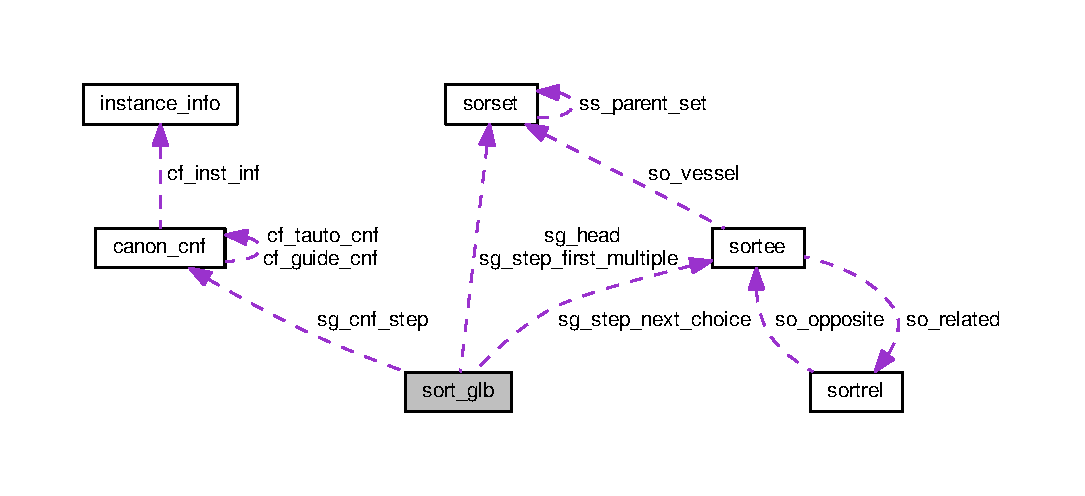
\includegraphics[width=350pt]{d8/d20/classsort__glb__coll__graph}
\end{center}
\end{figure}
\subsection*{Public Member Functions}
\begin{DoxyCompactItemize}
\item 
void \hyperlink{classsort__glb_ac755a6417f43e7860ca96317a8e8f4e8}{sort\+\_\+all\+\_\+from} (row$<$ \hyperlink{classsortee}{sortee} $\ast$ $>$ \&tees, sort\+\_\+id\+\_\+t curr\+\_\+id, bool add\+\_\+ccl\+\_\+id, long ccl\+\_\+id, bool sort\+\_\+opps, tgt\+\_\+ccl\+\_\+t tgt, \hyperlink{classsort__glb}{sort\+\_\+glb} $\ast$dbg\+\_\+srg=N\+U\+L\+L\+\_\+\+P\+T, \hyperlink{classsortee}{sortee} $\ast$dbg\+\_\+srt=N\+U\+L\+L\+\_\+\+P\+T)
\begin{DoxyCompactList}\small\item\em It calls \hyperlink{classsortee_a5cc113e22e62dfcb3869c2786ae5345e}{sortee\+::sort\+\_\+from} operations for all \hyperlink{classsortee}{sortee} s in tees. \end{DoxyCompactList}\item 
\hypertarget{classsort__glb_a25baf3b8e0bc9bdca9c0d6658b298f07}{void \hyperlink{classsort__glb_a25baf3b8e0bc9bdca9c0d6658b298f07}{step\+\_\+neus} (\hyperlink{classsort__glb}{sort\+\_\+glb} \&mates\+\_\+srg)}\label{classsort__glb_a25baf3b8e0bc9bdca9c0d6658b298f07}

\begin{DoxyCompactList}\small\item\em It does sort\+\_\+from operations on this \hyperlink{classsort__glb}{sort\+\_\+glb} \hyperlink{classneuron}{neuron} \hyperlink{classsortee}{sortee} s. \end{DoxyCompactList}\item 
\hypertarget{classsort__glb_a40a9304f2ef43071021472a8e020069a}{void \hyperlink{classsort__glb_a40a9304f2ef43071021472a8e020069a}{step\+\_\+opps} (\hyperlink{classsort__glb}{sort\+\_\+glb} \&mates\+\_\+srg)}\label{classsort__glb_a40a9304f2ef43071021472a8e020069a}

\begin{DoxyCompactList}\small\item\em It does sort\+\_\+from operations on this \hyperlink{classsort__glb}{sort\+\_\+glb} opposite \hyperlink{classquanton}{quanton} \hyperlink{classsortee}{sortee} s. \end{DoxyCompactList}\item 
\hypertarget{classsort__glb_aa41c7303e4bae7eb7c466f119c3ace1f}{void \hyperlink{classsort__glb_aa41c7303e4bae7eb7c466f119c3ace1f}{step\+\_\+quas} (\hyperlink{classsort__glb}{sort\+\_\+glb} \&mates\+\_\+srg)}\label{classsort__glb_aa41c7303e4bae7eb7c466f119c3ace1f}

\begin{DoxyCompactList}\small\item\em It does sort\+\_\+from operations on this \hyperlink{classsort__glb}{sort\+\_\+glb} \hyperlink{classquanton}{quanton} \hyperlink{classsortee}{sortee} s. \end{DoxyCompactList}\item 
void \hyperlink{classsort__glb_a314081679beafcbbeac7f2e504558f18}{stab\+\_\+mutual\+\_\+core} (\hyperlink{classsort__glb}{sort\+\_\+glb} \&mates\+\_\+srg)
\begin{DoxyCompactList}\small\item\em It stabilizes \hyperlink{classneuron}{neuron} \hyperlink{classsortee}{sortee} s and \hyperlink{classquanton}{quanton} \hyperlink{classsortee}{sortee} s until no further refinement is possible. \end{DoxyCompactList}\item 
void \hyperlink{classsort__glb_ad87061a8532cc773200ba06d939a6dfc}{stab\+\_\+mutual} (\hyperlink{classsort__glb}{sort\+\_\+glb} \&mates\+\_\+srg, bool one\+\_\+ccl\+\_\+per\+\_\+ss)
\begin{DoxyCompactList}\small\item\em It stabilizes two 'loaded' (initialized) \hyperlink{classsort__glb}{sort\+\_\+glb} with a \hyperlink{classneuromap}{neuromap} (no further refinement is possible). \end{DoxyCompactList}\item 
void \hyperlink{classsort__glb_abcd6c73d28df5efcf002c2aed63ccd92}{stab\+\_\+mutual\+\_\+unique} (\hyperlink{classsort__glb}{sort\+\_\+glb} \&mates\+\_\+srg, \hyperlink{classneuromap}{neuromap} $\ast$dbg\+\_\+nmp=N\+U\+L\+L\+\_\+\+P\+T)
\begin{DoxyCompactList}\small\item\em It stabilizes two 'loaded' (initialized) \hyperlink{classsort__glb}{sort\+\_\+glb} with a \hyperlink{classneuromap}{neuromap} to a B\+C\+F\+F. \end{DoxyCompactList}\end{DoxyCompactItemize}


\subsection{Detailed Description}
Class that holds all global data used to stabilize a group of items. 

Items are basically \hyperlink{classneuron}{neuron} s and \hyperlink{classquanton}{quanton} s representing a sub-\/formula of a C\+N\+F. This class does not handle \hyperlink{classneuron}{neuron} s and \hyperlink{classquanton}{quanton} s directly. Instead it handles their respective \hyperlink{classsortee}{sortee} s. 

\subsection{Member Function Documentation}
\hypertarget{classsort__glb_ac755a6417f43e7860ca96317a8e8f4e8}{\index{sort\+\_\+glb@{sort\+\_\+glb}!sort\+\_\+all\+\_\+from@{sort\+\_\+all\+\_\+from}}
\index{sort\+\_\+all\+\_\+from@{sort\+\_\+all\+\_\+from}!sort\+\_\+glb@{sort\+\_\+glb}}
\subsubsection[{sort\+\_\+all\+\_\+from}]{\setlength{\rightskip}{0pt plus 5cm}void sort\+\_\+glb\+::sort\+\_\+all\+\_\+from (
\begin{DoxyParamCaption}
\item[{row$<$ {\bf sortee} $\ast$ $>$ \&}]{tees, }
\item[{sort\+\_\+id\+\_\+t}]{curr\+\_\+id, }
\item[{bool}]{add\+\_\+ccl\+\_\+id, }
\item[{long}]{ccl\+\_\+id, }
\item[{bool}]{sort\+\_\+opps, }
\item[{tgt\+\_\+ccl\+\_\+t}]{tgt, }
\item[{{\bf sort\+\_\+glb} $\ast$}]{dbg\+\_\+srg = {\ttfamily NULL\+\_\+PT}, }
\item[{{\bf sortee} $\ast$}]{dbg\+\_\+srt = {\ttfamily NULL\+\_\+PT}}
\end{DoxyParamCaption}
)}}\label{classsort__glb_ac755a6417f43e7860ca96317a8e8f4e8}


It calls \hyperlink{classsortee_a5cc113e22e62dfcb3869c2786ae5345e}{sortee\+::sort\+\_\+from} operations for all \hyperlink{classsortee}{sortee} s in tees. 


\begin{DoxyParams}{Parameters}
{\em tees} & The \hyperlink{classsortee}{sortee} s to call \hyperlink{classsortee_a5cc113e22e62dfcb3869c2786ae5345e}{sortee\+::sort\+\_\+from}\+: \\
\hline
{\em curr\+\_\+id} & Current consecutive sorting id for this \hyperlink{classsort__glb}{sort\+\_\+glb}. \\
\hline
{\em add\+\_\+ccl\+\_\+id} & If true it appends ccl\+\_\+id to the so\+\_\+ccl field (a \hyperlink{classcanon__cnf}{canon\+\_\+cnf}) of each \hyperlink{classsortee}{sortee} in tees. \\
\hline
{\em ccl\+\_\+id} & The literal to be added to the B\+C\+F\+F if add\+\_\+ccl\+\_\+id is true. \\
\hline
{\em sort\+\_\+opps} & If true it uses de opposite of each \hyperlink{classsortee}{sortee} s in tees. \\
\hline
{\em tgt} & If (tgt != tc\+\_\+none) sg\+\_\+cnf\+\_\+dims for this \hyperlink{classsort__glb}{sort\+\_\+glb} is updated. \\
\hline
{\em dbg\+\_\+srg} & Auxsiliary param for debugging pourposes. \\
\hline
{\em dbg\+\_\+srt} & Auxsiliary param for debugging pourposes. \\
\hline
\end{DoxyParams}
\begin{DoxySeeAlso}{See also}
\hyperlink{macro__algorithm__ben__jose_8cpp}{macro\+\_\+algorithm\+\_\+ben\+\_\+jose.\+cpp} 
\end{DoxySeeAlso}
\hypertarget{classsort__glb_a314081679beafcbbeac7f2e504558f18}{\index{sort\+\_\+glb@{sort\+\_\+glb}!stab\+\_\+mutual\+\_\+core@{stab\+\_\+mutual\+\_\+core}}
\index{stab\+\_\+mutual\+\_\+core@{stab\+\_\+mutual\+\_\+core}!sort\+\_\+glb@{sort\+\_\+glb}}
\subsubsection[{stab\+\_\+mutual\+\_\+core}]{\setlength{\rightskip}{0pt plus 5cm}void sort\+\_\+glb\+::stab\+\_\+mutual\+\_\+core (
\begin{DoxyParamCaption}
\item[{{\bf sort\+\_\+glb} \&}]{srg2}
\end{DoxyParamCaption}
)}}\label{classsort__glb_a314081679beafcbbeac7f2e504558f18}


It stabilizes \hyperlink{classneuron}{neuron} \hyperlink{classsortee}{sortee} s and \hyperlink{classquanton}{quanton} \hyperlink{classsortee}{sortee} s until no further refinement is possible. 

\begin{DoxySeeAlso}{See also}
\hyperlink{macro__algorithm__ben__jose_8cpp}{macro\+\_\+algorithm\+\_\+ben\+\_\+jose.\+cpp} 
\end{DoxySeeAlso}


Here is the call graph for this function\+:\nopagebreak
\begin{figure}[H]
\begin{center}
\leavevmode
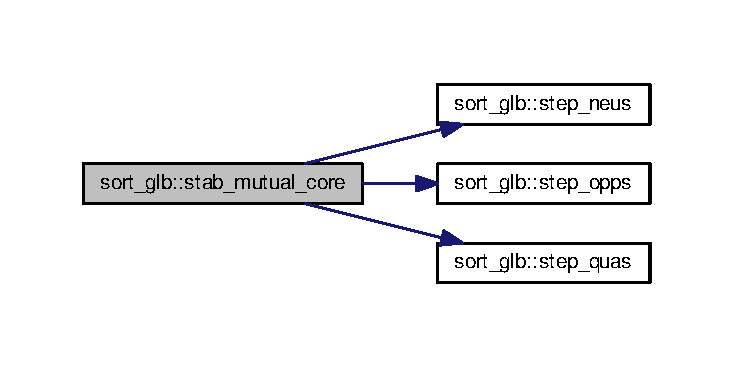
\includegraphics[width=350pt]{d7/dec/classsort__glb_a314081679beafcbbeac7f2e504558f18_cgraph}
\end{center}
\end{figure}




Here is the caller graph for this function\+:\nopagebreak
\begin{figure}[H]
\begin{center}
\leavevmode
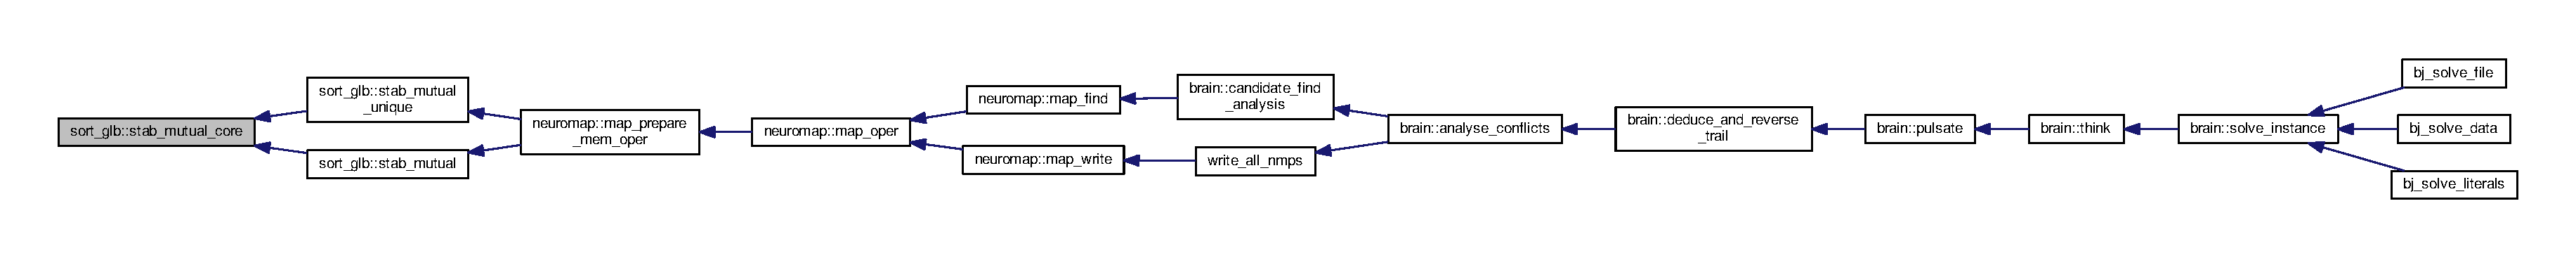
\includegraphics[width=350pt]{d7/dec/classsort__glb_a314081679beafcbbeac7f2e504558f18_icgraph}
\end{center}
\end{figure}


\hypertarget{classsort__glb_ad87061a8532cc773200ba06d939a6dfc}{\index{sort\+\_\+glb@{sort\+\_\+glb}!stab\+\_\+mutual@{stab\+\_\+mutual}}
\index{stab\+\_\+mutual@{stab\+\_\+mutual}!sort\+\_\+glb@{sort\+\_\+glb}}
\subsubsection[{stab\+\_\+mutual}]{\setlength{\rightskip}{0pt plus 5cm}void sort\+\_\+glb\+::stab\+\_\+mutual (
\begin{DoxyParamCaption}
\item[{{\bf sort\+\_\+glb} \&}]{srg2, }
\item[{bool}]{one\+\_\+ccl\+\_\+per\+\_\+ss}
\end{DoxyParamCaption}
)}}\label{classsort__glb_ad87061a8532cc773200ba06d939a6dfc}


It stabilizes two 'loaded' (initialized) \hyperlink{classsort__glb}{sort\+\_\+glb} with a \hyperlink{classneuromap}{neuromap} (no further refinement is possible). 

\begin{DoxySeeAlso}{See also}
\hyperlink{macro__algorithm__ben__jose_8cpp}{macro\+\_\+algorithm\+\_\+ben\+\_\+jose.\+cpp} 
\end{DoxySeeAlso}


Here is the call graph for this function\+:\nopagebreak
\begin{figure}[H]
\begin{center}
\leavevmode
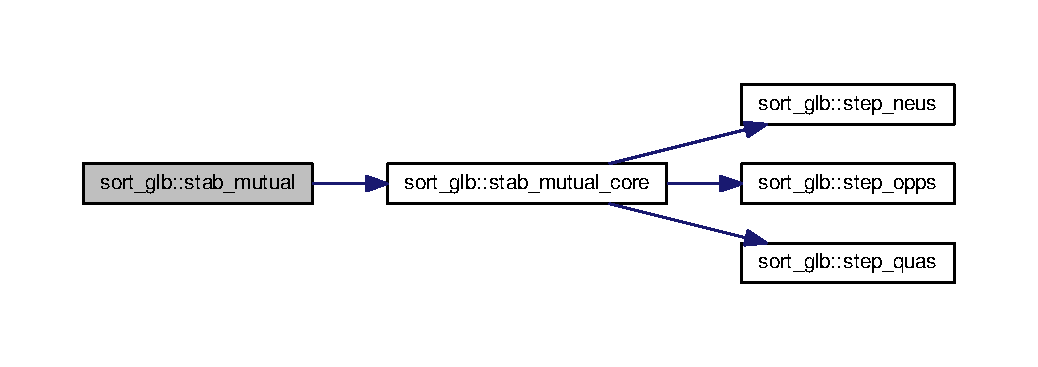
\includegraphics[width=350pt]{d7/dec/classsort__glb_ad87061a8532cc773200ba06d939a6dfc_cgraph}
\end{center}
\end{figure}




Here is the caller graph for this function\+:\nopagebreak
\begin{figure}[H]
\begin{center}
\leavevmode
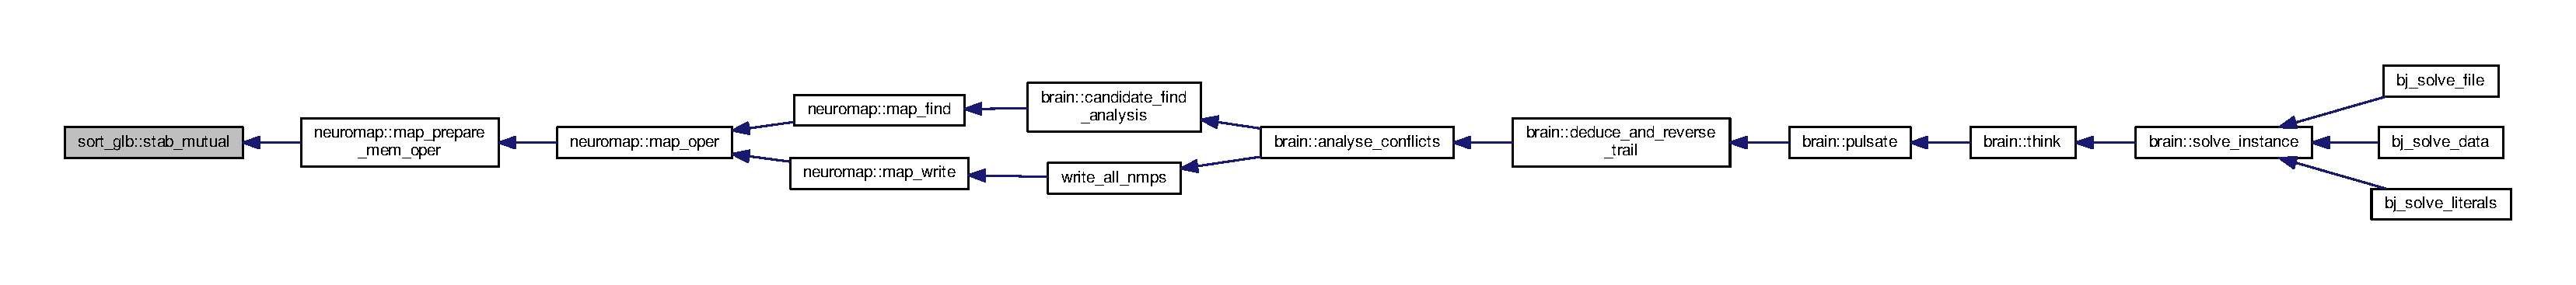
\includegraphics[width=350pt]{d7/dec/classsort__glb_ad87061a8532cc773200ba06d939a6dfc_icgraph}
\end{center}
\end{figure}


\hypertarget{classsort__glb_abcd6c73d28df5efcf002c2aed63ccd92}{\index{sort\+\_\+glb@{sort\+\_\+glb}!stab\+\_\+mutual\+\_\+unique@{stab\+\_\+mutual\+\_\+unique}}
\index{stab\+\_\+mutual\+\_\+unique@{stab\+\_\+mutual\+\_\+unique}!sort\+\_\+glb@{sort\+\_\+glb}}
\subsubsection[{stab\+\_\+mutual\+\_\+unique}]{\setlength{\rightskip}{0pt plus 5cm}void sort\+\_\+glb\+::stab\+\_\+mutual\+\_\+unique (
\begin{DoxyParamCaption}
\item[{{\bf sort\+\_\+glb} \&}]{srg2, }
\item[{{\bf neuromap} $\ast$}]{dbg\+\_\+nmp = {\ttfamily NULL\+\_\+PT}}
\end{DoxyParamCaption}
)}}\label{classsort__glb_abcd6c73d28df5efcf002c2aed63ccd92}


It stabilizes two 'loaded' (initialized) \hyperlink{classsort__glb}{sort\+\_\+glb} with a \hyperlink{classneuromap}{neuromap} to a B\+C\+F\+F. 

\begin{DoxySeeAlso}{See also}
\hyperlink{macro__algorithm__ben__jose_8cpp}{macro\+\_\+algorithm\+\_\+ben\+\_\+jose.\+cpp} 
\end{DoxySeeAlso}


Here is the call graph for this function\+:\nopagebreak
\begin{figure}[H]
\begin{center}
\leavevmode
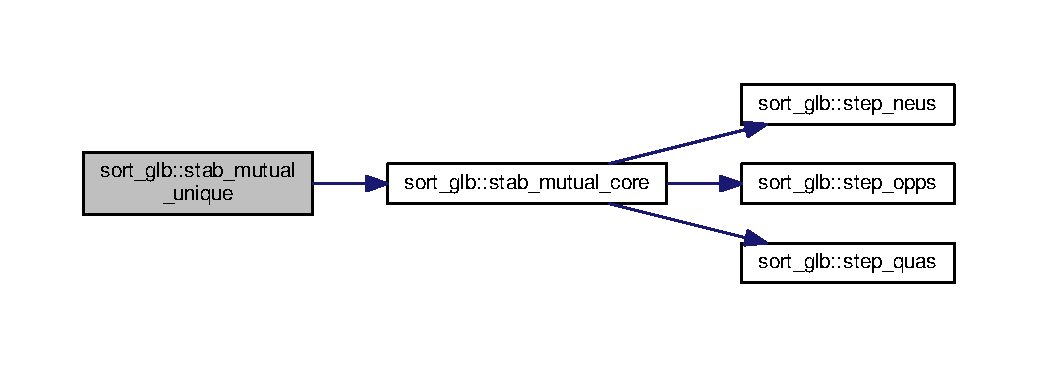
\includegraphics[width=350pt]{d7/dec/classsort__glb_abcd6c73d28df5efcf002c2aed63ccd92_cgraph}
\end{center}
\end{figure}




Here is the caller graph for this function\+:\nopagebreak
\begin{figure}[H]
\begin{center}
\leavevmode
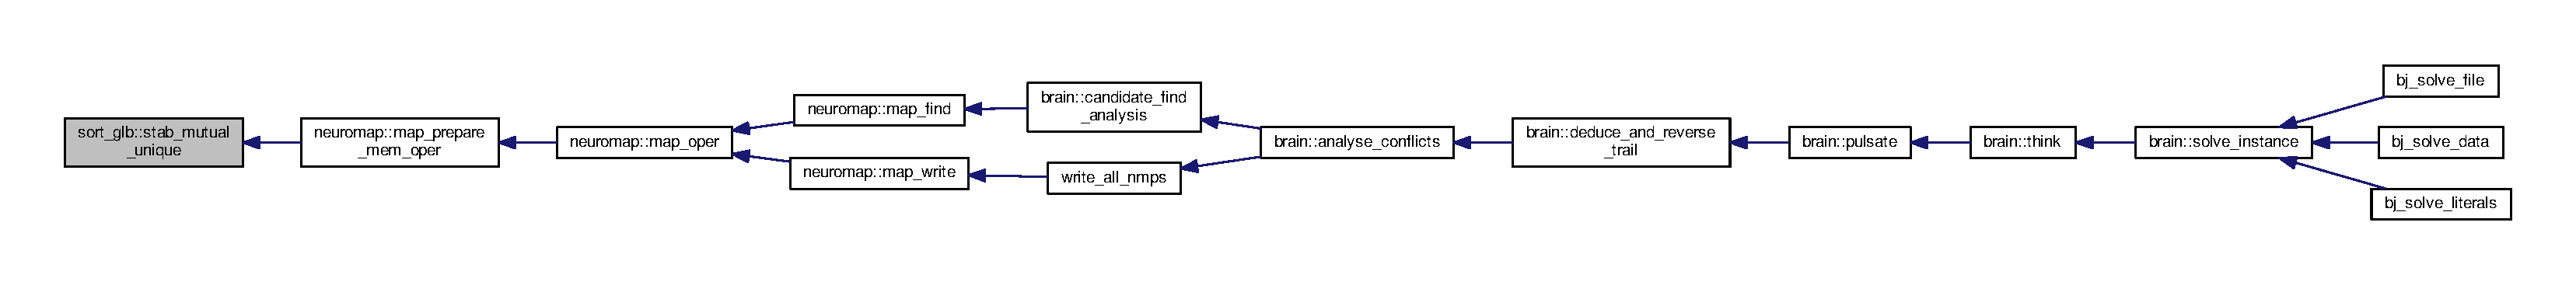
\includegraphics[width=350pt]{d7/dec/classsort__glb_abcd6c73d28df5efcf002c2aed63ccd92_icgraph}
\end{center}
\end{figure}




The documentation for this class was generated from the following files\+:\begin{DoxyCompactItemize}
\item 
/home/jose/devel/ben-\/jose/src/library/brain/sortor.\+h\item 
/home/jose/devel/ben-\/jose/src/library/api/macro\+\_\+ben\+\_\+jose.\+cpp\item 
/home/jose/devel/ben-\/jose/src/library/brain/sortor.\+cpp\item 
/home/jose/devel/ben-\/jose/src/programs/macro\+\_\+ben\+\_\+jose/\hyperlink{macro__algorithm__ben__jose_8cpp}{macro\+\_\+algorithm\+\_\+ben\+\_\+jose.\+cpp}\end{DoxyCompactItemize}

\hypertarget{classsortee}{}\section{sortee Class Reference}
\label{classsortee}\index{sortee@{sortee}}


Class that is an item to be stabilized.  




{\ttfamily \#include $<$sortor.\+h$>$}



Inherits binder.



Collaboration diagram for sortee\+:
% FIG 0
\subsection*{Public Member Functions}
\begin{DoxyCompactItemize}
\item 
void \hyperlink{classsortee_a5cc113e22e62dfcb3869c2786ae5345e}{sort\+\_\+from} (\hyperlink{classsort__glb}{sort\+\_\+glb} \&srg, sort\+\_\+id\+\_\+t curr\+\_\+nid, void $\ast$id\+\_\+src=N\+U\+L\+L\+\_\+\+PT)
\begin{DoxyCompactList}\small\item\em The basic stabilization step finds the next \hyperlink{classsorset}{sorset} and puts this \hyperlink{classsortee}{sortee} in it. \end{DoxyCompactList}\end{DoxyCompactItemize}


\subsection{Detailed Description}
Class that is an item to be stabilized. 

Each \hyperlink{classneuron}{neuron} contains one \hyperlink{classsortee}{sortee} and each \hyperlink{classquanton}{quanton} contains one \hyperlink{classsortee}{sortee}. Each \hyperlink{classsortee}{sortee} \textquotesingle{}knows\textquotesingle{} (void pointer) which \hyperlink{classneuron}{neuron} or \hyperlink{classquanton}{quanton} contains it. It is a one-\/to-\/one relation that is used to stabilize C\+NF sub-\/formulas. During stabilization, the \hyperlink{classsort__glb}{sort\+\_\+glb} handles the \hyperlink{classsortee}{sortee} s not the \hyperlink{classneuron}{neuron} s and \hyperlink{classquanton}{quanton} s. containing them. 

\subsection{Member Function Documentation}
\index{sortee@{sortee}!sort\+\_\+from@{sort\+\_\+from}}
\index{sort\+\_\+from@{sort\+\_\+from}!sortee@{sortee}}
\subsubsection[{\texorpdfstring{sort\+\_\+from(sort\+\_\+glb \&srg, sort\+\_\+id\+\_\+t curr\+\_\+nid, void $\ast$id\+\_\+src=\+N\+U\+L\+L\+\_\+\+P\+T)}{sort_from(sort_glb &srg, sort_id_t curr_nid, void *id_src=NULL_PT)}}]{\setlength{\rightskip}{0pt plus 5cm}void sortee\+::sort\+\_\+from (
\begin{DoxyParamCaption}
\item[{{\bf sort\+\_\+glb} \&}]{srg, }
\item[{sort\+\_\+id\+\_\+t}]{curr\+\_\+id, }
\item[{void $\ast$}]{id\+\_\+src = {\ttfamily NULL\+\_\+PT}}
\end{DoxyParamCaption}
)}\hypertarget{classsortee_a5cc113e22e62dfcb3869c2786ae5345e}{}\label{classsortee_a5cc113e22e62dfcb3869c2786ae5345e}


The basic stabilization step finds the next \hyperlink{classsorset}{sorset} and puts this \hyperlink{classsortee}{sortee} in it. 

\begin{DoxySeeAlso}{See also}
\hyperlink{macro__algorithm__ben__jose_8cpp}{macro\+\_\+algorithm\+\_\+ben\+\_\+jose.\+cpp} 
\end{DoxySeeAlso}


Here is the caller graph for this function\+:
% FIG 1




The documentation for this class was generated from the following files\+:\begin{DoxyCompactItemize}
\item 
/home/jose/devel/ben-\/jose/src/library/brain/sortor.\+h\item 
/home/jose/devel/ben-\/jose/src/library/brain/sortor.\+cpp\end{DoxyCompactItemize}

\hypertarget{classsortrel}{}\section{sortrel Class Reference}
\label{classsortrel}\index{sortrel@{sortrel}}


A sortrel is a relation between two \hyperlink{classsortee}{sortee} s.  




{\ttfamily \#include $<$sortor.\+h$>$}



Collaboration diagram for sortrel\+:
% FIG 0


\subsection{Detailed Description}
A sortrel is a relation between two \hyperlink{classsortee}{sortee} s. 

It represents a relation between two \hyperlink{classsortee}{sortee} s. In our case every \hyperlink{classsortee}{sortee} representing a \hyperlink{classneuron}{neuron} holds one \hyperlink{classsortrel}{sortrel} per fiber (literal), and each \hyperlink{classsortee}{sortee} representing a \hyperlink{classquanton}{quanton} holds one \hyperlink{classsortrel}{sortrel} per \hyperlink{classneuron}{neuron} in wick the \hyperlink{classquanton}{quanton} is found. They must be properly initiated before each stabilization. They define the stabilizing sub-\/formula\textquotesingle{}s relations between it\textquotesingle{}s \hyperlink{classneuron}{neuron} s and \hyperlink{classquanton}{quanton} s by relating their respective \hyperlink{classsortee}{sortee} s. They represent relations between a particular sub group (sub-\/formula) of \hyperlink{classneuron}{neuron} \textquotesingle{}s \hyperlink{classsortee}{sortee} s and \hyperlink{classquanton}{quanton} \textquotesingle{}s \hyperlink{classsortee}{sortee} s. 

The documentation for this class was generated from the following file\+:\begin{DoxyCompactItemize}
\item 
/home/jose/devel/ben-\/jose/src/library/brain/sortor.\+h\end{DoxyCompactItemize}

\chapter{File Documentation}
\hypertarget{ben__jose_8cpp}{}\section{/home/jose/devel/ben-\/jose/src/library/api/ben\+\_\+jose.cpp File Reference}
\label{ben__jose_8cpp}\index{/home/jose/devel/ben-\/jose/src/library/api/ben\+\_\+jose.\+cpp@{/home/jose/devel/ben-\/jose/src/library/api/ben\+\_\+jose.\+cpp}}


File containing the implementation code for the users A\+PI of ben\+\_\+jose.  


{\ttfamily \#include $<$cstdio$>$}\\*
{\ttfamily \#include \char`\"{}ben\+\_\+jose.\+h\char`\"{}}\\*
{\ttfamily \#include \char`\"{}brain.\+h\char`\"{}}\\*
{\ttfamily \#include \char`\"{}solver.\+h\char`\"{}}\\*
{\ttfamily \#include \char`\"{}file\+\_\+funcs.\+h\char`\"{}}\\*
{\ttfamily \#include \char`\"{}dbg\+\_\+prt.\+h\char`\"{}}\\*
Include dependency graph for ben\+\_\+jose.\+cpp\+:
\nopagebreak
\begin{figure}[H]
\begin{center}
\leavevmode
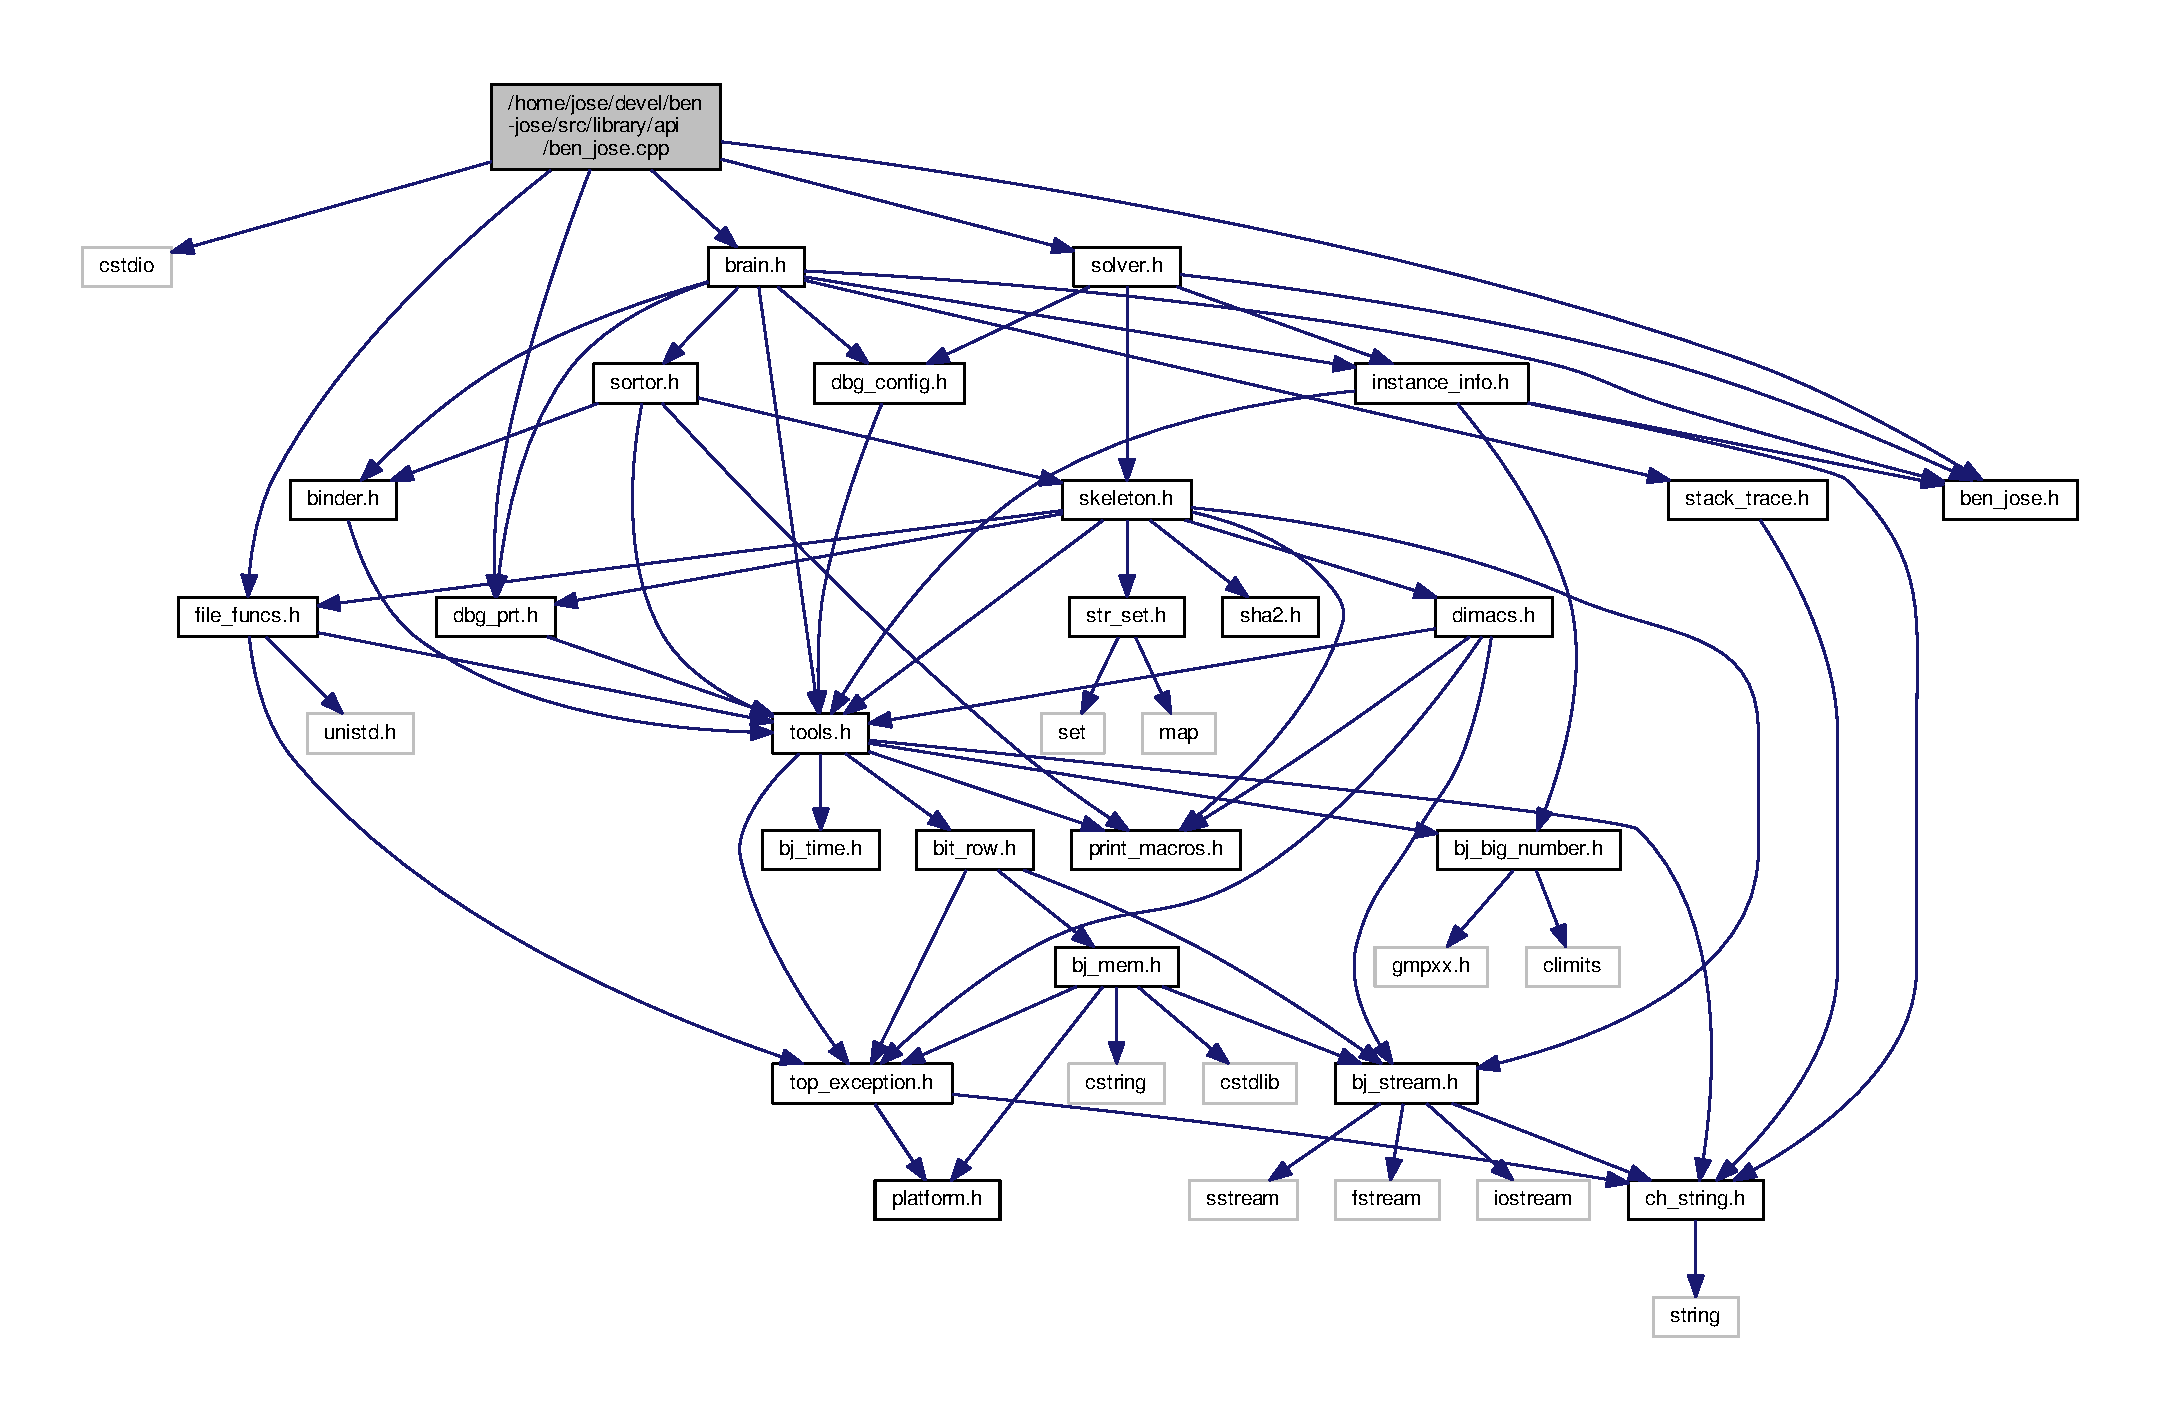
\includegraphics[width=350pt]{d2/d50/ben__jose_8cpp__incl}
\end{center}
\end{figure}
\subsection*{Functions}
\begin{DoxyCompactItemize}
\item 
void \hyperlink{ben__jose_8cpp_a017fab7c4a46c76367a8810a6a0da452}{bj\+\_\+init\+\_\+output} (bj\+\_\+output\+\_\+t $\ast$the\+\_\+out)
\item 
\hyperlink{ben__jose_8h_a3825fe3519107001ca4d0679f1d0a110}{bj\+\_\+solver\+\_\+t} \hyperlink{ben__jose_8cpp_a3f6cb5e5aac2da12b2d475c81909becf}{bj\+\_\+solver\+\_\+create} (const char $\ast$bjs\+\_\+dir\+\_\+path)
\item 
void \hyperlink{ben__jose_8cpp_ae256ffb1a6f33249d57c88ad79c5132b}{bj\+\_\+solver\+\_\+release} (\hyperlink{ben__jose_8h_a3825fe3519107001ca4d0679f1d0a110}{bj\+\_\+solver\+\_\+t} bjs)
\item 
void \hyperlink{ben__jose_8cpp_afeb4622efbaae0a207b9d0a394b860ee}{bj\+\_\+set\+\_\+param\+\_\+char} (\hyperlink{ben__jose_8h_a3825fe3519107001ca4d0679f1d0a110}{bj\+\_\+solver\+\_\+t} bjs, \hyperlink{group__docgrp___a_p_i_gadb76574300f22fca6a209194e0254e29}{bj\+\_\+param\+\_\+t} prm, char val)
\item 
char \hyperlink{ben__jose_8cpp_ae5e07f54c5d1f3315695876d31bbfc4d}{bj\+\_\+get\+\_\+param\+\_\+char} (\hyperlink{ben__jose_8h_a3825fe3519107001ca4d0679f1d0a110}{bj\+\_\+solver\+\_\+t} bjs, \hyperlink{group__docgrp___a_p_i_gadb76574300f22fca6a209194e0254e29}{bj\+\_\+param\+\_\+t} prm)
\item 
const char $\ast$ \hyperlink{ben__jose_8cpp_aacdcf2c366bfd31c06c00cb33a548e9f}{bj\+\_\+get\+\_\+database\+\_\+path} (\hyperlink{ben__jose_8h_a3825fe3519107001ca4d0679f1d0a110}{bj\+\_\+solver\+\_\+t} bjs)
\item 
\hyperlink{group__docgrp___a_p_i_ga9aba221730ab694a549d25ee1aa28c69}{bj\+\_\+satisf\+\_\+val\+\_\+t} \hyperlink{ben__jose_8cpp_a65eb23939cc4ae39654dbd93343580c8}{bj\+\_\+solve\+\_\+file} (\hyperlink{ben__jose_8h_a3825fe3519107001ca4d0679f1d0a110}{bj\+\_\+solver\+\_\+t} bjs, const char $\ast$f\+\_\+path)
\item 
\hyperlink{group__docgrp___a_p_i_ga9aba221730ab694a549d25ee1aa28c69}{bj\+\_\+satisf\+\_\+val\+\_\+t} \hyperlink{ben__jose_8cpp_a45eef575a2ca6c6b90e0a1d998f1eb7d}{bj\+\_\+solve\+\_\+data} (\hyperlink{ben__jose_8h_a3825fe3519107001ca4d0679f1d0a110}{bj\+\_\+solver\+\_\+t} bjs, long dat\+\_\+sz, const char $\ast$dat)
\item 
\hyperlink{group__docgrp___a_p_i_ga9aba221730ab694a549d25ee1aa28c69}{bj\+\_\+satisf\+\_\+val\+\_\+t} \hyperlink{ben__jose_8cpp_a2818f32df95b8d462f49a201ce371142}{bj\+\_\+solve\+\_\+literals} (\hyperlink{ben__jose_8h_a3825fe3519107001ca4d0679f1d0a110}{bj\+\_\+solver\+\_\+t} bjs, long num\+\_\+vars, long num\+\_\+cls, long lits\+\_\+sz, long $\ast$lits)
\item 
\hyperlink{group__docgrp___a_p_i_ga9aba221730ab694a549d25ee1aa28c69}{bj\+\_\+satisf\+\_\+val\+\_\+t} \hyperlink{ben__jose_8cpp_aef97ca0385d43a4415e6710d07b1dd4d}{bj\+\_\+get\+\_\+result} (\hyperlink{ben__jose_8h_a3825fe3519107001ca4d0679f1d0a110}{bj\+\_\+solver\+\_\+t} bjs)
\item 
bj\+\_\+output\+\_\+t \hyperlink{ben__jose_8cpp_a2685b092d0a891b280bc1895d1deaef1}{bj\+\_\+get\+\_\+output} (\hyperlink{ben__jose_8h_a3825fe3519107001ca4d0679f1d0a110}{bj\+\_\+solver\+\_\+t} bjs)
\item 
const char $\ast$ \hyperlink{ben__jose_8cpp_a2cd47bfce4c972f1882857eb7910569d}{bj\+\_\+get\+\_\+solve\+\_\+file\+\_\+path} (\hyperlink{ben__jose_8h_a3825fe3519107001ca4d0679f1d0a110}{bj\+\_\+solver\+\_\+t} bjs)
\item 
const long $\ast$ \hyperlink{ben__jose_8cpp_a672cdf8b8774c4224e1cd641f0460705}{bj\+\_\+get\+\_\+assig} (\hyperlink{ben__jose_8h_a3825fe3519107001ca4d0679f1d0a110}{bj\+\_\+solver\+\_\+t} bjs)
\item 
const char $\ast$ \hyperlink{ben__jose_8cpp_ac3cb476b34f135c0370047bc5ade0058}{bj\+\_\+get\+\_\+last\+\_\+proof\+\_\+path} (\hyperlink{ben__jose_8h_a3825fe3519107001ca4d0679f1d0a110}{bj\+\_\+solver\+\_\+t} bjs)
\item 
const char $\ast$ \hyperlink{ben__jose_8cpp_abf18e6ff43cc5a12b15d6317da5357ef}{bj\+\_\+get\+\_\+error\+\_\+stack\+\_\+str} (\hyperlink{ben__jose_8h_a3825fe3519107001ca4d0679f1d0a110}{bj\+\_\+solver\+\_\+t} bjs)
\item 
const char $\ast$ \hyperlink{ben__jose_8cpp_aa74202918cc8ec8e05d541a9fa04251f}{bj\+\_\+get\+\_\+error\+\_\+assert\+\_\+str} (\hyperlink{ben__jose_8h_a3825fe3519107001ca4d0679f1d0a110}{bj\+\_\+solver\+\_\+t} bjs)
\item 
void \hyperlink{ben__jose_8cpp_a62d44e173c8c8d19dae9c88696649127}{bj\+\_\+restart} (\hyperlink{ben__jose_8h_a3825fe3519107001ca4d0679f1d0a110}{bj\+\_\+solver\+\_\+t} bjs)
\item 
void \hyperlink{ben__jose_8cpp_ac7ff7cedad8c30e85232f52cb1c6e716}{bj\+\_\+print\+\_\+paths} (\hyperlink{ben__jose_8h_a3825fe3519107001ca4d0679f1d0a110}{bj\+\_\+solver\+\_\+t} bjs)
\item 
const char $\ast$ \hyperlink{ben__jose_8cpp_ab6303f60ba14cddd8b534b40830df31d}{bj\+\_\+error\+\_\+str} (\hyperlink{group__docgrp___a_p_i_ga92a0ce4b68a949f501a3b1d4fb1ded8b}{bj\+\_\+error\+\_\+t} bje)
\item 
const char $\ast$ \hyperlink{ben__jose_8cpp_a09f75c893eb86496a7fa1eba093b9d67}{bj\+\_\+get\+\_\+result\+\_\+titles\+\_\+string} (\hyperlink{ben__jose_8h_a3825fe3519107001ca4d0679f1d0a110}{bj\+\_\+solver\+\_\+t} bjs)
\item 
const char $\ast$ \hyperlink{ben__jose_8cpp_aef3c645a9b041d6f7fd7aa720d255308}{bj\+\_\+get\+\_\+result\+\_\+string} (\hyperlink{ben__jose_8h_a3825fe3519107001ca4d0679f1d0a110}{bj\+\_\+solver\+\_\+t} bjs)
\item 
void \hyperlink{ben__jose_8cpp_ac23228b810b4eadd052ee3dcc193a0a5}{bj\+\_\+parse\+\_\+result\+\_\+string} (\hyperlink{ben__jose_8h_a3825fe3519107001ca4d0679f1d0a110}{bj\+\_\+solver\+\_\+t} bjs, const char $\ast$rslt\+\_\+str)
\end{DoxyCompactItemize}


\subsection{Detailed Description}
File containing the implementation code for the users A\+PI of ben\+\_\+jose. 









\subsection{Function Documentation}
\index{ben\+\_\+jose.\+cpp@{ben\+\_\+jose.\+cpp}!bj\+\_\+init\+\_\+output@{bj\+\_\+init\+\_\+output}}
\index{bj\+\_\+init\+\_\+output@{bj\+\_\+init\+\_\+output}!ben\+\_\+jose.\+cpp@{ben\+\_\+jose.\+cpp}}
\subsubsection[{\texorpdfstring{bj\+\_\+init\+\_\+output(bj\+\_\+output\+\_\+t $\ast$the\+\_\+out)}{bj_init_output(bj_output_t *the_out)}}]{\setlength{\rightskip}{0pt plus 5cm}void bj\+\_\+init\+\_\+output (
\begin{DoxyParamCaption}
\item[{bj\+\_\+output\+\_\+t $\ast$}]{the\+\_\+out}
\end{DoxyParamCaption}
)}\hypertarget{ben__jose_8cpp_a017fab7c4a46c76367a8810a6a0da452}{}\label{ben__jose_8cpp_a017fab7c4a46c76367a8810a6a0da452}
Init a bj\+\_\+output\+\_\+t structure 
\begin{DoxyParams}{Parameters}
{\em the\+\_\+out} & A pointer to the structure to be initialized \\
\hline
\end{DoxyParams}


Here is the call graph for this function\+:
\nopagebreak
\begin{figure}[H]
\begin{center}
\leavevmode
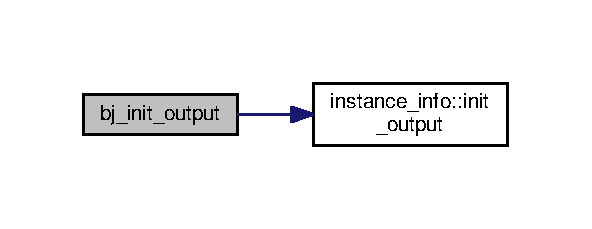
\includegraphics[width=284pt]{d1/d55/ben__jose_8cpp_a017fab7c4a46c76367a8810a6a0da452_cgraph}
\end{center}
\end{figure}


\index{ben\+\_\+jose.\+cpp@{ben\+\_\+jose.\+cpp}!bj\+\_\+solver\+\_\+create@{bj\+\_\+solver\+\_\+create}}
\index{bj\+\_\+solver\+\_\+create@{bj\+\_\+solver\+\_\+create}!ben\+\_\+jose.\+cpp@{ben\+\_\+jose.\+cpp}}
\subsubsection[{\texorpdfstring{bj\+\_\+solver\+\_\+create(const char $\ast$bjs\+\_\+dir\+\_\+path)}{bj_solver_create(const char *bjs_dir_path)}}]{\setlength{\rightskip}{0pt plus 5cm}{\bf bj\+\_\+solver\+\_\+t} bj\+\_\+solver\+\_\+create (
\begin{DoxyParamCaption}
\item[{const char $\ast$}]{bjs\+\_\+dir\+\_\+path}
\end{DoxyParamCaption}
)}\hypertarget{ben__jose_8cpp_a3f6cb5e5aac2da12b2d475c81909becf}{}\label{ben__jose_8cpp_a3f6cb5e5aac2da12b2d475c81909becf}
Create a solver object to solve one or more C\+N\+Fs 
\begin{DoxyParams}{Parameters}
{\em bjs\+\_\+dir\+\_\+path} & A C string that represents the path of the database of C\+N\+Fs. \\
\hline
\end{DoxyParams}
\begin{DoxyReturn}{Returns}
A bj\+\_\+solver\+\_\+t object representing a solver. 
\end{DoxyReturn}
\index{ben\+\_\+jose.\+cpp@{ben\+\_\+jose.\+cpp}!bj\+\_\+solver\+\_\+release@{bj\+\_\+solver\+\_\+release}}
\index{bj\+\_\+solver\+\_\+release@{bj\+\_\+solver\+\_\+release}!ben\+\_\+jose.\+cpp@{ben\+\_\+jose.\+cpp}}
\subsubsection[{\texorpdfstring{bj\+\_\+solver\+\_\+release(bj\+\_\+solver\+\_\+t bjs)}{bj_solver_release(bj_solver_t bjs)}}]{\setlength{\rightskip}{0pt plus 5cm}void bj\+\_\+solver\+\_\+release (
\begin{DoxyParamCaption}
\item[{{\bf bj\+\_\+solver\+\_\+t}}]{bjs}
\end{DoxyParamCaption}
)}\hypertarget{ben__jose_8cpp_ae256ffb1a6f33249d57c88ad79c5132b}{}\label{ben__jose_8cpp_ae256ffb1a6f33249d57c88ad79c5132b}
Release a solver object created with bj\+\_\+solver\+\_\+create 
\begin{DoxyParams}{Parameters}
{\em bjs} & The solver object to be released. \\
\hline
\end{DoxyParams}
\index{ben\+\_\+jose.\+cpp@{ben\+\_\+jose.\+cpp}!bj\+\_\+set\+\_\+param\+\_\+char@{bj\+\_\+set\+\_\+param\+\_\+char}}
\index{bj\+\_\+set\+\_\+param\+\_\+char@{bj\+\_\+set\+\_\+param\+\_\+char}!ben\+\_\+jose.\+cpp@{ben\+\_\+jose.\+cpp}}
\subsubsection[{\texorpdfstring{bj\+\_\+set\+\_\+param\+\_\+char(bj\+\_\+solver\+\_\+t bjs, bj\+\_\+param\+\_\+t prm, char val)}{bj_set_param_char(bj_solver_t bjs, bj_param_t prm, char val)}}]{\setlength{\rightskip}{0pt plus 5cm}void bj\+\_\+set\+\_\+param\+\_\+char (
\begin{DoxyParamCaption}
\item[{{\bf bj\+\_\+solver\+\_\+t}}]{bjs, }
\item[{{\bf bj\+\_\+param\+\_\+t}}]{prm, }
\item[{char}]{val}
\end{DoxyParamCaption}
)}\hypertarget{ben__jose_8cpp_afeb4622efbaae0a207b9d0a394b860ee}{}\label{ben__jose_8cpp_afeb4622efbaae0a207b9d0a394b860ee}
Set an input parameter in the solver 
\begin{DoxyParams}{Parameters}
{\em bjs} & The solver object to be used. \\
\hline
{\em prm} & The parameter. \\
\hline
{\em val} & The value. For boolen values it is 0 (false) or not 0 (true) \\
\hline
\end{DoxyParams}
\index{ben\+\_\+jose.\+cpp@{ben\+\_\+jose.\+cpp}!bj\+\_\+get\+\_\+param\+\_\+char@{bj\+\_\+get\+\_\+param\+\_\+char}}
\index{bj\+\_\+get\+\_\+param\+\_\+char@{bj\+\_\+get\+\_\+param\+\_\+char}!ben\+\_\+jose.\+cpp@{ben\+\_\+jose.\+cpp}}
\subsubsection[{\texorpdfstring{bj\+\_\+get\+\_\+param\+\_\+char(bj\+\_\+solver\+\_\+t bjs, bj\+\_\+param\+\_\+t prm)}{bj_get_param_char(bj_solver_t bjs, bj_param_t prm)}}]{\setlength{\rightskip}{0pt plus 5cm}char bj\+\_\+get\+\_\+param\+\_\+char (
\begin{DoxyParamCaption}
\item[{{\bf bj\+\_\+solver\+\_\+t}}]{bjs, }
\item[{{\bf bj\+\_\+param\+\_\+t}}]{prm}
\end{DoxyParamCaption}
)}\hypertarget{ben__jose_8cpp_ae5e07f54c5d1f3315695876d31bbfc4d}{}\label{ben__jose_8cpp_ae5e07f54c5d1f3315695876d31bbfc4d}
Get the value of a previusly set (with bj\+\_\+set\+\_\+param\+\_\+char) input parameter. 
\begin{DoxyParams}{Parameters}
{\em bjs} & The solver object to be used. \\
\hline
{\em prm} & The parameter. \\
\hline
\end{DoxyParams}
\begin{DoxyReturn}{Returns}
The value. For boolen values it is 0 (false) or 1 (true) 
\end{DoxyReturn}
\index{ben\+\_\+jose.\+cpp@{ben\+\_\+jose.\+cpp}!bj\+\_\+get\+\_\+database\+\_\+path@{bj\+\_\+get\+\_\+database\+\_\+path}}
\index{bj\+\_\+get\+\_\+database\+\_\+path@{bj\+\_\+get\+\_\+database\+\_\+path}!ben\+\_\+jose.\+cpp@{ben\+\_\+jose.\+cpp}}
\subsubsection[{\texorpdfstring{bj\+\_\+get\+\_\+database\+\_\+path(bj\+\_\+solver\+\_\+t bjs)}{bj_get_database_path(bj_solver_t bjs)}}]{\setlength{\rightskip}{0pt plus 5cm}const char$\ast$ bj\+\_\+get\+\_\+database\+\_\+path (
\begin{DoxyParamCaption}
\item[{{\bf bj\+\_\+solver\+\_\+t}}]{bjs}
\end{DoxyParamCaption}
)}\hypertarget{ben__jose_8cpp_aacdcf2c366bfd31c06c00cb33a548e9f}{}\label{ben__jose_8cpp_aacdcf2c366bfd31c06c00cb33a548e9f}
Get the value of a previusly set database path (with bj\+\_\+solver\+\_\+create). 
\begin{DoxyParams}{Parameters}
{\em bjs} & The solver object to be used. \\
\hline
\end{DoxyParams}
\begin{DoxyReturn}{Returns}
The database directory path. Do not free the returned pointer. 
\end{DoxyReturn}
\index{ben\+\_\+jose.\+cpp@{ben\+\_\+jose.\+cpp}!bj\+\_\+solve\+\_\+file@{bj\+\_\+solve\+\_\+file}}
\index{bj\+\_\+solve\+\_\+file@{bj\+\_\+solve\+\_\+file}!ben\+\_\+jose.\+cpp@{ben\+\_\+jose.\+cpp}}
\subsubsection[{\texorpdfstring{bj\+\_\+solve\+\_\+file(bj\+\_\+solver\+\_\+t bjs, const char $\ast$f\+\_\+path)}{bj_solve_file(bj_solver_t bjs, const char *f_path)}}]{\setlength{\rightskip}{0pt plus 5cm}{\bf bj\+\_\+satisf\+\_\+val\+\_\+t} bj\+\_\+solve\+\_\+file (
\begin{DoxyParamCaption}
\item[{{\bf bj\+\_\+solver\+\_\+t}}]{bjs, }
\item[{const char $\ast$}]{f\+\_\+path}
\end{DoxyParamCaption}
)}\hypertarget{ben__jose_8cpp_a65eb23939cc4ae39654dbd93343580c8}{}\label{ben__jose_8cpp_a65eb23939cc4ae39654dbd93343580c8}
Solve a C\+NF given the D\+I\+M\+A\+CS formated file path of the C\+NF. 
\begin{DoxyParams}{Parameters}
{\em bjs} & The solver object to be used. \\
\hline
{\em f\+\_\+path} & The C\+NF file path. It must be in D\+I\+M\+A\+CS format. \\
\hline
\end{DoxyParams}
\begin{DoxyReturn}{Returns}
The solving result. 
\end{DoxyReturn}


Here is the call graph for this function\+:
\nopagebreak
\begin{figure}[H]
\begin{center}
\leavevmode
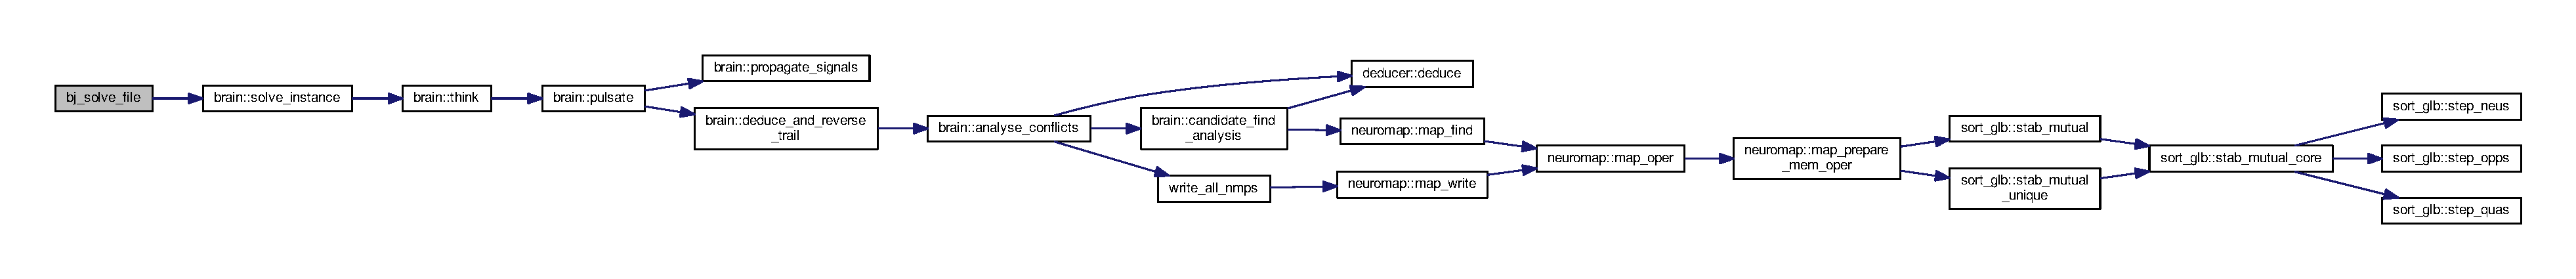
\includegraphics[width=350pt]{d1/d55/ben__jose_8cpp_a65eb23939cc4ae39654dbd93343580c8_cgraph}
\end{center}
\end{figure}


\index{ben\+\_\+jose.\+cpp@{ben\+\_\+jose.\+cpp}!bj\+\_\+solve\+\_\+data@{bj\+\_\+solve\+\_\+data}}
\index{bj\+\_\+solve\+\_\+data@{bj\+\_\+solve\+\_\+data}!ben\+\_\+jose.\+cpp@{ben\+\_\+jose.\+cpp}}
\subsubsection[{\texorpdfstring{bj\+\_\+solve\+\_\+data(bj\+\_\+solver\+\_\+t bjs, long dat\+\_\+sz, const char $\ast$dat)}{bj_solve_data(bj_solver_t bjs, long dat_sz, const char *dat)}}]{\setlength{\rightskip}{0pt plus 5cm}{\bf bj\+\_\+satisf\+\_\+val\+\_\+t} bj\+\_\+solve\+\_\+data (
\begin{DoxyParamCaption}
\item[{{\bf bj\+\_\+solver\+\_\+t}}]{bjs, }
\item[{long}]{dat\+\_\+sz, }
\item[{const char $\ast$}]{dat}
\end{DoxyParamCaption}
)}\hypertarget{ben__jose_8cpp_a45eef575a2ca6c6b90e0a1d998f1eb7d}{}\label{ben__jose_8cpp_a45eef575a2ca6c6b90e0a1d998f1eb7d}
Solve a C\+NF given a D\+I\+M\+A\+CS formated C A\+S\+C\+II characters array. 
\begin{DoxyParams}{Parameters}
{\em bjs} & The solver object to be used. \\
\hline
{\em dat\+\_\+sz} & The number of A\+S\+C\+II characters in dat. \\
\hline
{\em dat} & The D\+I\+M\+A\+CS formated C A\+S\+C\+II characters array. It can be the exact contents read of a valid D\+I\+M\+A\+CS file. \\
\hline
\end{DoxyParams}
\begin{DoxyReturn}{Returns}
The solving result. 
\end{DoxyReturn}


Here is the call graph for this function\+:
\nopagebreak
\begin{figure}[H]
\begin{center}
\leavevmode
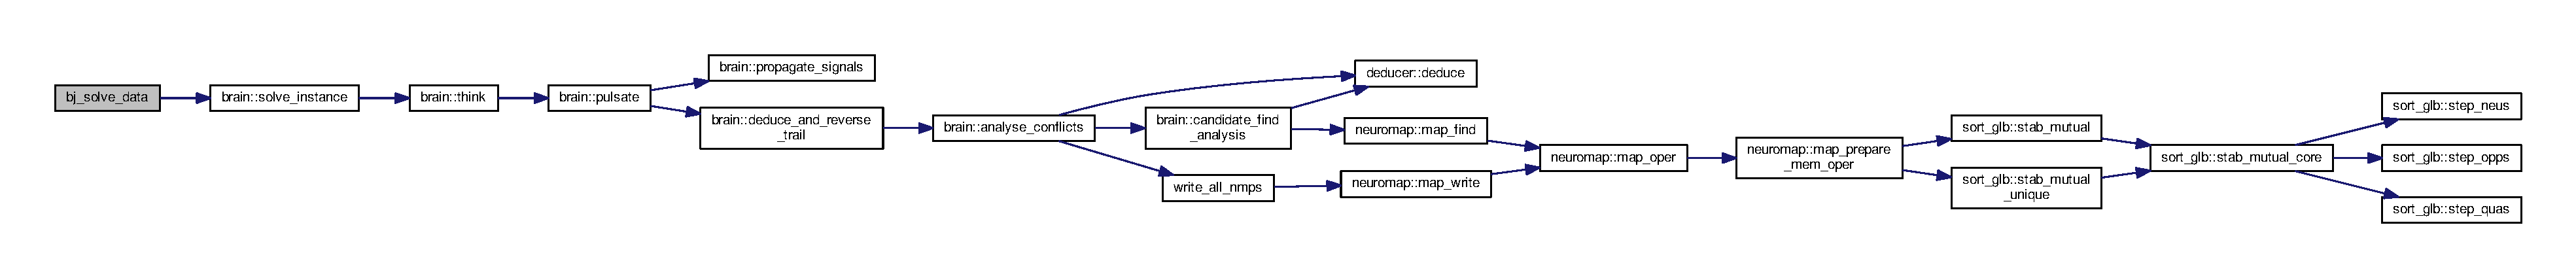
\includegraphics[width=350pt]{d1/d55/ben__jose_8cpp_a45eef575a2ca6c6b90e0a1d998f1eb7d_cgraph}
\end{center}
\end{figure}


\index{ben\+\_\+jose.\+cpp@{ben\+\_\+jose.\+cpp}!bj\+\_\+solve\+\_\+literals@{bj\+\_\+solve\+\_\+literals}}
\index{bj\+\_\+solve\+\_\+literals@{bj\+\_\+solve\+\_\+literals}!ben\+\_\+jose.\+cpp@{ben\+\_\+jose.\+cpp}}
\subsubsection[{\texorpdfstring{bj\+\_\+solve\+\_\+literals(bj\+\_\+solver\+\_\+t bjs, long num\+\_\+vars, long num\+\_\+cls, long lits\+\_\+sz, long $\ast$lits)}{bj_solve_literals(bj_solver_t bjs, long num_vars, long num_cls, long lits_sz, long *lits)}}]{\setlength{\rightskip}{0pt plus 5cm}{\bf bj\+\_\+satisf\+\_\+val\+\_\+t} bj\+\_\+solve\+\_\+literals (
\begin{DoxyParamCaption}
\item[{{\bf bj\+\_\+solver\+\_\+t}}]{bjs, }
\item[{long}]{num\+\_\+vars, }
\item[{long}]{num\+\_\+cls, }
\item[{long}]{lits\+\_\+sz, }
\item[{long $\ast$}]{lits}
\end{DoxyParamCaption}
)}\hypertarget{ben__jose_8cpp_a2818f32df95b8d462f49a201ce371142}{}\label{ben__jose_8cpp_a2818f32df95b8d462f49a201ce371142}
Solve a C\+NF given the D\+I\+M\+A\+CS values of a C\+NF. 
\begin{DoxyParams}{Parameters}
{\em bjs} & The solver object to be used. \\
\hline
{\em num\+\_\+vars} & The number of variables in used in lits. It is the value as read in a cnf declaration of a D\+I\+M\+A\+CS file. \\
\hline
{\em num\+\_\+cls} & The number of clauses found in lits. It is the value as read in a cnf declaration of a D\+I\+M\+A\+CS file. \\
\hline
{\em lits\+\_\+sz} & The size of the lits parameter. \\
\hline
{\em lits} & T\+He array containing a set of clauses separated by zeros. Ej\+: \mbox{[}1 2 0 3 4 5 0\mbox{]} representes two clauses\+: \mbox{[}1 2\mbox{]} and \mbox{[}3 4 5\mbox{]}. \\
\hline
\end{DoxyParams}
\begin{DoxyReturn}{Returns}
The solving result. 
\end{DoxyReturn}


Here is the call graph for this function\+:
\nopagebreak
\begin{figure}[H]
\begin{center}
\leavevmode
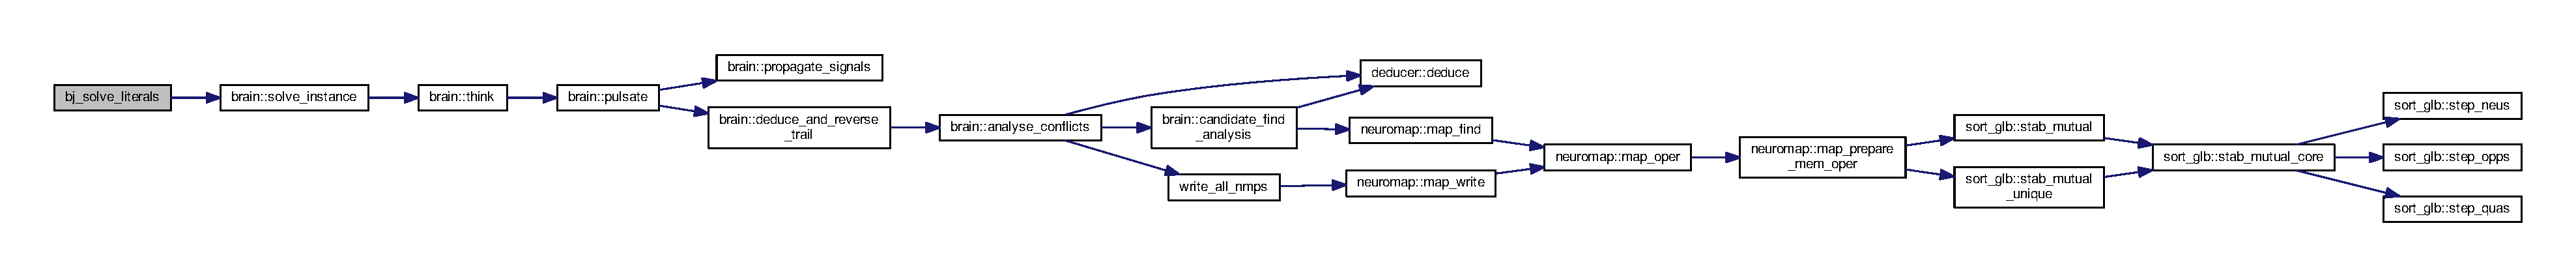
\includegraphics[width=350pt]{d1/d55/ben__jose_8cpp_a2818f32df95b8d462f49a201ce371142_cgraph}
\end{center}
\end{figure}


\index{ben\+\_\+jose.\+cpp@{ben\+\_\+jose.\+cpp}!bj\+\_\+get\+\_\+result@{bj\+\_\+get\+\_\+result}}
\index{bj\+\_\+get\+\_\+result@{bj\+\_\+get\+\_\+result}!ben\+\_\+jose.\+cpp@{ben\+\_\+jose.\+cpp}}
\subsubsection[{\texorpdfstring{bj\+\_\+get\+\_\+result(bj\+\_\+solver\+\_\+t bjs)}{bj_get_result(bj_solver_t bjs)}}]{\setlength{\rightskip}{0pt plus 5cm}{\bf bj\+\_\+satisf\+\_\+val\+\_\+t} bj\+\_\+get\+\_\+result (
\begin{DoxyParamCaption}
\item[{{\bf bj\+\_\+solver\+\_\+t}}]{bjs}
\end{DoxyParamCaption}
)}\hypertarget{ben__jose_8cpp_aef97ca0385d43a4415e6710d07b1dd4d}{}\label{ben__jose_8cpp_aef97ca0385d43a4415e6710d07b1dd4d}
Get the result of a solving process. A bj\+\_\+solve\+\_\+ function must have been previusly called. 
\begin{DoxyParams}{Parameters}
{\em bjs} & The solver object to be used. \\
\hline
\end{DoxyParams}
\begin{DoxyReturn}{Returns}
The solving result. It has the same value returned by the previusly called bj\+\_\+solve\+\_\+ function. 
\end{DoxyReturn}
\index{ben\+\_\+jose.\+cpp@{ben\+\_\+jose.\+cpp}!bj\+\_\+get\+\_\+output@{bj\+\_\+get\+\_\+output}}
\index{bj\+\_\+get\+\_\+output@{bj\+\_\+get\+\_\+output}!ben\+\_\+jose.\+cpp@{ben\+\_\+jose.\+cpp}}
\subsubsection[{\texorpdfstring{bj\+\_\+get\+\_\+output(bj\+\_\+solver\+\_\+t bjs)}{bj_get_output(bj_solver_t bjs)}}]{\setlength{\rightskip}{0pt plus 5cm}bj\+\_\+output\+\_\+t bj\+\_\+get\+\_\+output (
\begin{DoxyParamCaption}
\item[{{\bf bj\+\_\+solver\+\_\+t}}]{bjs}
\end{DoxyParamCaption}
)}\hypertarget{ben__jose_8cpp_a2685b092d0a891b280bc1895d1deaef1}{}\label{ben__jose_8cpp_a2685b092d0a891b280bc1895d1deaef1}
Get all the output a solving process. A bj\+\_\+solve\+\_\+ function must have been previusly called. 
\begin{DoxyParams}{Parameters}
{\em bjs} & The solver object to be used. \\
\hline
\end{DoxyParams}
\begin{DoxyReturn}{Returns}
The solving output. 
\end{DoxyReturn}
\begin{DoxySeeAlso}{See also}
bj\+\_\+output\+\_\+t 
\end{DoxySeeAlso}


Here is the call graph for this function\+:
\nopagebreak
\begin{figure}[H]
\begin{center}
\leavevmode
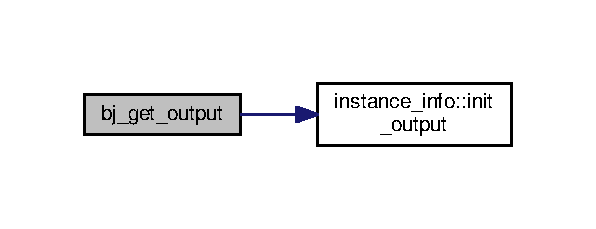
\includegraphics[width=286pt]{d1/d55/ben__jose_8cpp_a2685b092d0a891b280bc1895d1deaef1_cgraph}
\end{center}
\end{figure}


\index{ben\+\_\+jose.\+cpp@{ben\+\_\+jose.\+cpp}!bj\+\_\+get\+\_\+solve\+\_\+file\+\_\+path@{bj\+\_\+get\+\_\+solve\+\_\+file\+\_\+path}}
\index{bj\+\_\+get\+\_\+solve\+\_\+file\+\_\+path@{bj\+\_\+get\+\_\+solve\+\_\+file\+\_\+path}!ben\+\_\+jose.\+cpp@{ben\+\_\+jose.\+cpp}}
\subsubsection[{\texorpdfstring{bj\+\_\+get\+\_\+solve\+\_\+file\+\_\+path(bj\+\_\+solver\+\_\+t bjs)}{bj_get_solve_file_path(bj_solver_t bjs)}}]{\setlength{\rightskip}{0pt plus 5cm}const char$\ast$ bj\+\_\+get\+\_\+solve\+\_\+file\+\_\+path (
\begin{DoxyParamCaption}
\item[{{\bf bj\+\_\+solver\+\_\+t}}]{bjs}
\end{DoxyParamCaption}
)}\hypertarget{ben__jose_8cpp_a2cd47bfce4c972f1882857eb7910569d}{}\label{ben__jose_8cpp_a2cd47bfce4c972f1882857eb7910569d}
Returns the value passed to bj\+\_\+solve\+\_\+file. A bj\+\_\+solve\+\_\+ function must have been previusly called. 
\begin{DoxyParams}{Parameters}
{\em bjs} & The solver object to be used. \\
\hline
\end{DoxyParams}
\begin{DoxyReturn}{Returns}
The value passed to bj\+\_\+solve\+\_\+file or null otherwise (other bj\+\_\+solve\+\_\+ function was called). 
\end{DoxyReturn}
\index{ben\+\_\+jose.\+cpp@{ben\+\_\+jose.\+cpp}!bj\+\_\+get\+\_\+assig@{bj\+\_\+get\+\_\+assig}}
\index{bj\+\_\+get\+\_\+assig@{bj\+\_\+get\+\_\+assig}!ben\+\_\+jose.\+cpp@{ben\+\_\+jose.\+cpp}}
\subsubsection[{\texorpdfstring{bj\+\_\+get\+\_\+assig(bj\+\_\+solver\+\_\+t bjs)}{bj_get_assig(bj_solver_t bjs)}}]{\setlength{\rightskip}{0pt plus 5cm}const long$\ast$ bj\+\_\+get\+\_\+assig (
\begin{DoxyParamCaption}
\item[{{\bf bj\+\_\+solver\+\_\+t}}]{bjs}
\end{DoxyParamCaption}
)}\hypertarget{ben__jose_8cpp_a672cdf8b8774c4224e1cd641f0460705}{}\label{ben__jose_8cpp_a672cdf8b8774c4224e1cd641f0460705}
Get the assignation to variables that satisfies the C\+NF. A bj\+\_\+solve\+\_\+ function must have been previusly called. 
\begin{DoxyParams}{Parameters}
{\em bjs} & The solver object to be used. \\
\hline
\end{DoxyParams}
\begin{DoxyReturn}{Returns}
An array (here called \textquotesingle{}assig\textquotesingle{}) with the assignation to variables that satisfies the C\+NF.
\end{DoxyReturn}
\textquotesingle{}assig\textquotesingle{} always ends with a 0.

No memory after that 0 should be accessed.

Let vv = assig\mbox{[}ii\mbox{]}. Then\+:


\begin{DoxyItemize}
\item If vv is positive it means the the variable represented by abs(vv) is assigned true
\item If vv is negative it means the the variable represented by abs(vv) is assigned false
\end{DoxyItemize}

Example\+: \mbox{[}-\/20 4 -\/12 6 9 0\mbox{]}

Means\+:
\begin{DoxyItemize}
\item set var 20 to false
\item set var 4 to true
\item set var 12 to false
\item set var 6 to true
\item set var 9 to true
\end{DoxyItemize}

And that assignation satisfies the whole C\+NF (it might have more than 20 variables). \index{ben\+\_\+jose.\+cpp@{ben\+\_\+jose.\+cpp}!bj\+\_\+get\+\_\+last\+\_\+proof\+\_\+path@{bj\+\_\+get\+\_\+last\+\_\+proof\+\_\+path}}
\index{bj\+\_\+get\+\_\+last\+\_\+proof\+\_\+path@{bj\+\_\+get\+\_\+last\+\_\+proof\+\_\+path}!ben\+\_\+jose.\+cpp@{ben\+\_\+jose.\+cpp}}
\subsubsection[{\texorpdfstring{bj\+\_\+get\+\_\+last\+\_\+proof\+\_\+path(bj\+\_\+solver\+\_\+t bjs)}{bj_get_last_proof_path(bj_solver_t bjs)}}]{\setlength{\rightskip}{0pt plus 5cm}const char$\ast$ bj\+\_\+get\+\_\+last\+\_\+proof\+\_\+path (
\begin{DoxyParamCaption}
\item[{{\bf bj\+\_\+solver\+\_\+t}}]{bjs}
\end{DoxyParamCaption}
)}\hypertarget{ben__jose_8cpp_ac3cb476b34f135c0370047bc5ade0058}{}\label{ben__jose_8cpp_ac3cb476b34f135c0370047bc5ade0058}
Returns the last written proof path. A bj\+\_\+solve\+\_\+ function must have been previusly called. 
\begin{DoxyParams}{Parameters}
{\em bjs} & The solver object to be used. \\
\hline
\end{DoxyParams}
\begin{DoxyReturn}{Returns}
The path to the last written G\+S\+ON proof file.
\end{DoxyReturn}
N\+U\+LL is returned if the parameter bjp\+\_\+write\+\_\+proofs was not used before calling a bj\+\_\+solve\+\_\+ function. \index{ben\+\_\+jose.\+cpp@{ben\+\_\+jose.\+cpp}!bj\+\_\+get\+\_\+error\+\_\+stack\+\_\+str@{bj\+\_\+get\+\_\+error\+\_\+stack\+\_\+str}}
\index{bj\+\_\+get\+\_\+error\+\_\+stack\+\_\+str@{bj\+\_\+get\+\_\+error\+\_\+stack\+\_\+str}!ben\+\_\+jose.\+cpp@{ben\+\_\+jose.\+cpp}}
\subsubsection[{\texorpdfstring{bj\+\_\+get\+\_\+error\+\_\+stack\+\_\+str(bj\+\_\+solver\+\_\+t bjs)}{bj_get_error_stack_str(bj_solver_t bjs)}}]{\setlength{\rightskip}{0pt plus 5cm}const char$\ast$ bj\+\_\+get\+\_\+error\+\_\+stack\+\_\+str (
\begin{DoxyParamCaption}
\item[{{\bf bj\+\_\+solver\+\_\+t}}]{bjs}
\end{DoxyParamCaption}
)}\hypertarget{ben__jose_8cpp_abf18e6ff43cc5a12b15d6317da5357ef}{}\label{ben__jose_8cpp_abf18e6ff43cc5a12b15d6317da5357ef}
Get the stack when the error ocurred. A bj\+\_\+solve\+\_\+ function must have been previusly called. 
\begin{DoxyParams}{Parameters}
{\em bjs} & The solver object to be used. \\
\hline
\end{DoxyParams}
\begin{DoxyReturn}{Returns}
The stack when the error ocurred.
\end{DoxyReturn}
Funtion for debugging purposes. Only returns a valid value if an error has ocurred during solving. \index{ben\+\_\+jose.\+cpp@{ben\+\_\+jose.\+cpp}!bj\+\_\+get\+\_\+error\+\_\+assert\+\_\+str@{bj\+\_\+get\+\_\+error\+\_\+assert\+\_\+str}}
\index{bj\+\_\+get\+\_\+error\+\_\+assert\+\_\+str@{bj\+\_\+get\+\_\+error\+\_\+assert\+\_\+str}!ben\+\_\+jose.\+cpp@{ben\+\_\+jose.\+cpp}}
\subsubsection[{\texorpdfstring{bj\+\_\+get\+\_\+error\+\_\+assert\+\_\+str(bj\+\_\+solver\+\_\+t bjs)}{bj_get_error_assert_str(bj_solver_t bjs)}}]{\setlength{\rightskip}{0pt plus 5cm}const char$\ast$ bj\+\_\+get\+\_\+error\+\_\+assert\+\_\+str (
\begin{DoxyParamCaption}
\item[{{\bf bj\+\_\+solver\+\_\+t}}]{bjs}
\end{DoxyParamCaption}
)}\hypertarget{ben__jose_8cpp_aa74202918cc8ec8e05d541a9fa04251f}{}\label{ben__jose_8cpp_aa74202918cc8ec8e05d541a9fa04251f}
Get the assert that failed. A bj\+\_\+solve\+\_\+ function must have been previusly called. 
\begin{DoxyParams}{Parameters}
{\em bjs} & The solver object to be used. \\
\hline
\end{DoxyParams}
\begin{DoxyReturn}{Returns}
The assert that failed.
\end{DoxyReturn}
Funtion for debugging purposes. Only returns a valid value if an assert has failed. \index{ben\+\_\+jose.\+cpp@{ben\+\_\+jose.\+cpp}!bj\+\_\+restart@{bj\+\_\+restart}}
\index{bj\+\_\+restart@{bj\+\_\+restart}!ben\+\_\+jose.\+cpp@{ben\+\_\+jose.\+cpp}}
\subsubsection[{\texorpdfstring{bj\+\_\+restart(bj\+\_\+solver\+\_\+t bjs)}{bj_restart(bj_solver_t bjs)}}]{\setlength{\rightskip}{0pt plus 5cm}void bj\+\_\+restart (
\begin{DoxyParamCaption}
\item[{{\bf bj\+\_\+solver\+\_\+t}}]{bjs}
\end{DoxyParamCaption}
)}\hypertarget{ben__jose_8cpp_a62d44e173c8c8d19dae9c88696649127}{}\label{ben__jose_8cpp_a62d44e173c8c8d19dae9c88696649127}
Resets all internal values in the solver. 
\begin{DoxyParams}{Parameters}
{\em bjs} & The solver object to be used. \\
\hline
\end{DoxyParams}
\index{ben\+\_\+jose.\+cpp@{ben\+\_\+jose.\+cpp}!bj\+\_\+print\+\_\+paths@{bj\+\_\+print\+\_\+paths}}
\index{bj\+\_\+print\+\_\+paths@{bj\+\_\+print\+\_\+paths}!ben\+\_\+jose.\+cpp@{ben\+\_\+jose.\+cpp}}
\subsubsection[{\texorpdfstring{bj\+\_\+print\+\_\+paths(bj\+\_\+solver\+\_\+t bjs)}{bj_print_paths(bj_solver_t bjs)}}]{\setlength{\rightskip}{0pt plus 5cm}void bj\+\_\+print\+\_\+paths (
\begin{DoxyParamCaption}
\item[{{\bf bj\+\_\+solver\+\_\+t}}]{bjs}
\end{DoxyParamCaption}
)}\hypertarget{ben__jose_8cpp_ac7ff7cedad8c30e85232f52cb1c6e716}{}\label{ben__jose_8cpp_ac7ff7cedad8c30e85232f52cb1c6e716}
Prints all paths used by the solver. 
\begin{DoxyParams}{Parameters}
{\em bjs} & The solver object to be used. \\
\hline
\end{DoxyParams}
\index{ben\+\_\+jose.\+cpp@{ben\+\_\+jose.\+cpp}!bj\+\_\+error\+\_\+str@{bj\+\_\+error\+\_\+str}}
\index{bj\+\_\+error\+\_\+str@{bj\+\_\+error\+\_\+str}!ben\+\_\+jose.\+cpp@{ben\+\_\+jose.\+cpp}}
\subsubsection[{\texorpdfstring{bj\+\_\+error\+\_\+str(bj\+\_\+error\+\_\+t bje)}{bj_error_str(bj_error_t bje)}}]{\setlength{\rightskip}{0pt plus 5cm}const char$\ast$ bj\+\_\+error\+\_\+str (
\begin{DoxyParamCaption}
\item[{{\bf bj\+\_\+error\+\_\+t}}]{bje}
\end{DoxyParamCaption}
)}\hypertarget{ben__jose_8cpp_ab6303f60ba14cddd8b534b40830df31d}{}\label{ben__jose_8cpp_ab6303f60ba14cddd8b534b40830df31d}
Gets a string representing the error. A bj\+\_\+solve\+\_\+ function must have been previusly called. 
\begin{DoxyParams}{Parameters}
{\em bjs} & The solver object to be used. \\
\hline
\end{DoxyParams}
\begin{DoxyReturn}{Returns}
A string representing the error. 
\end{DoxyReturn}
\index{ben\+\_\+jose.\+cpp@{ben\+\_\+jose.\+cpp}!bj\+\_\+get\+\_\+result\+\_\+titles\+\_\+string@{bj\+\_\+get\+\_\+result\+\_\+titles\+\_\+string}}
\index{bj\+\_\+get\+\_\+result\+\_\+titles\+\_\+string@{bj\+\_\+get\+\_\+result\+\_\+titles\+\_\+string}!ben\+\_\+jose.\+cpp@{ben\+\_\+jose.\+cpp}}
\subsubsection[{\texorpdfstring{bj\+\_\+get\+\_\+result\+\_\+titles\+\_\+string(bj\+\_\+solver\+\_\+t bjs)}{bj_get_result_titles_string(bj_solver_t bjs)}}]{\setlength{\rightskip}{0pt plus 5cm}const char$\ast$ bj\+\_\+get\+\_\+result\+\_\+titles\+\_\+string (
\begin{DoxyParamCaption}
\item[{{\bf bj\+\_\+solver\+\_\+t}}]{bjs}
\end{DoxyParamCaption}
)}\hypertarget{ben__jose_8cpp_a09f75c893eb86496a7fa1eba093b9d67}{}\label{ben__jose_8cpp_a09f75c893eb86496a7fa1eba093b9d67}
Get a string with the titles of a result string fields. 
\begin{DoxyParams}{Parameters}
{\em bjs} & The solver object to be used. \\
\hline
\end{DoxyParams}
\begin{DoxyReturn}{Returns}
A string with the titles of a result string fields.
\end{DoxyReturn}
Funtion for testing purposes. \index{ben\+\_\+jose.\+cpp@{ben\+\_\+jose.\+cpp}!bj\+\_\+get\+\_\+result\+\_\+string@{bj\+\_\+get\+\_\+result\+\_\+string}}
\index{bj\+\_\+get\+\_\+result\+\_\+string@{bj\+\_\+get\+\_\+result\+\_\+string}!ben\+\_\+jose.\+cpp@{ben\+\_\+jose.\+cpp}}
\subsubsection[{\texorpdfstring{bj\+\_\+get\+\_\+result\+\_\+string(bj\+\_\+solver\+\_\+t bjs)}{bj_get_result_string(bj_solver_t bjs)}}]{\setlength{\rightskip}{0pt plus 5cm}const char$\ast$ bj\+\_\+get\+\_\+result\+\_\+string (
\begin{DoxyParamCaption}
\item[{{\bf bj\+\_\+solver\+\_\+t}}]{bjs}
\end{DoxyParamCaption}
)}\hypertarget{ben__jose_8cpp_aef3c645a9b041d6f7fd7aa720d255308}{}\label{ben__jose_8cpp_aef3c645a9b041d6f7fd7aa720d255308}
Get a string with the result string. A bj\+\_\+solve\+\_\+ function must have been previusly called. 
\begin{DoxyParams}{Parameters}
{\em bjs} & The solver object to be used. \\
\hline
\end{DoxyParams}
\begin{DoxyReturn}{Returns}
A string with the result string.
\end{DoxyReturn}
Funtion for testing purposes. It contains a concatenation of the string representation of some fields obtained otherwise with the bj\+\_\+get\+\_\+output funtion. \index{ben\+\_\+jose.\+cpp@{ben\+\_\+jose.\+cpp}!bj\+\_\+parse\+\_\+result\+\_\+string@{bj\+\_\+parse\+\_\+result\+\_\+string}}
\index{bj\+\_\+parse\+\_\+result\+\_\+string@{bj\+\_\+parse\+\_\+result\+\_\+string}!ben\+\_\+jose.\+cpp@{ben\+\_\+jose.\+cpp}}
\subsubsection[{\texorpdfstring{bj\+\_\+parse\+\_\+result\+\_\+string(bj\+\_\+solver\+\_\+t bjs, const char $\ast$rslt\+\_\+str)}{bj_parse_result_string(bj_solver_t bjs, const char *rslt_str)}}]{\setlength{\rightskip}{0pt plus 5cm}void bj\+\_\+parse\+\_\+result\+\_\+string (
\begin{DoxyParamCaption}
\item[{{\bf bj\+\_\+solver\+\_\+t}}]{bjs, }
\item[{const char $\ast$}]{rslt\+\_\+str}
\end{DoxyParamCaption}
)}\hypertarget{ben__jose_8cpp_ac23228b810b4eadd052ee3dcc193a0a5}{}\label{ben__jose_8cpp_ac23228b810b4eadd052ee3dcc193a0a5}
Sets internal values in the solver with a result string previusly returned by bj\+\_\+get\+\_\+result\+\_\+string. 
\begin{DoxyParams}{Parameters}
{\em bjs} & The solver object to be used. \\
\hline
{\em rslt\+\_\+str} & A string with the result string.\\
\hline
\end{DoxyParams}
Funtion for testing purposes. It sets internal values in the solver so that a call to bj\+\_\+get\+\_\+output will return the parsed values. 
\hypertarget{ben__jose_8h}{\section{/home/jose/devel/ben-\/jose/src/library/api/ben\+\_\+jose.h File Reference}
\label{ben__jose_8h}\index{/home/jose/devel/ben-\/jose/src/library/api/ben\+\_\+jose.\+h@{/home/jose/devel/ben-\/jose/src/library/api/ben\+\_\+jose.\+h}}
}


ben\+\_\+jose A\+P\+I declaration.  


This graph shows which files directly or indirectly include this file\+:\nopagebreak
\begin{figure}[H]
\begin{center}
\leavevmode
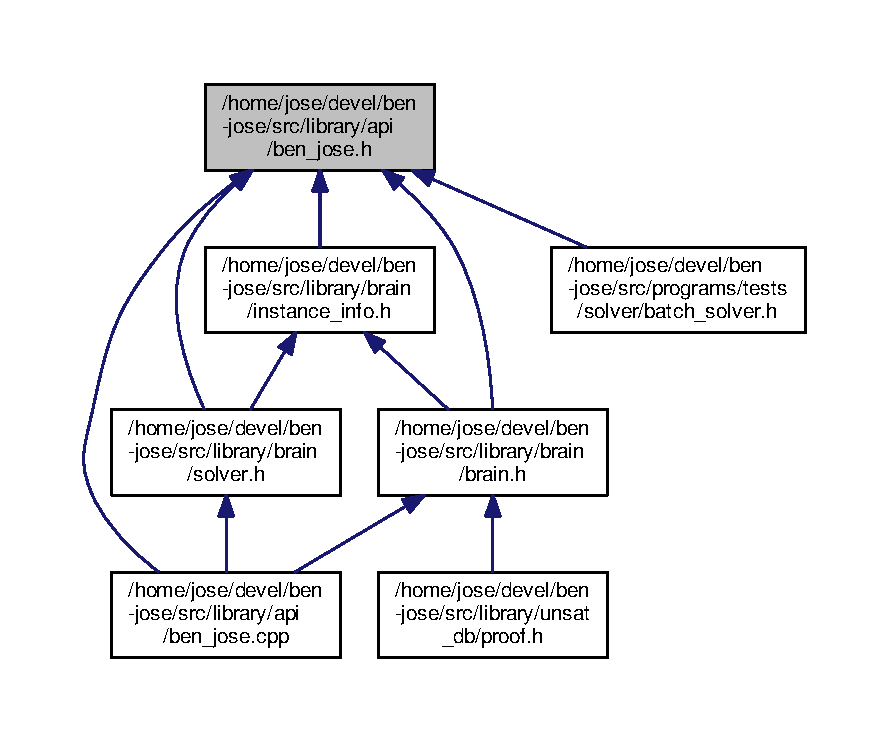
\includegraphics[width=350pt]{de/db7/ben__jose_8h__dep__incl}
\end{center}
\end{figure}
\subsection*{Macros}
\begin{DoxyCompactItemize}
\item 
\hypertarget{ben__jose_8h_a0a72e970c3c8ac4f24063140419ab702}{\#define \hyperlink{ben__jose_8h_a0a72e970c3c8ac4f24063140419ab702}{R\+E\+S\+\_\+\+U\+N\+K\+N\+O\+W\+N\+\_\+\+S\+T\+R}~\char`\"{}unknown\char`\"{}}\label{ben__jose_8h_a0a72e970c3c8ac4f24063140419ab702}

\begin{DoxyCompactList}\small\item\em String to print a \hyperlink{ben__jose_8h_ga9aba221730ab694a549d25ee1aa28c69ad8dafe2640a5e989a73880526a853663}{bjr\+\_\+unknown\+\_\+satisf} result. \end{DoxyCompactList}\item 
\hypertarget{ben__jose_8h_ac76e086f02ed4a2ba6db37b2aa5ec67d}{\#define \hyperlink{ben__jose_8h_ac76e086f02ed4a2ba6db37b2aa5ec67d}{bj\+\_\+solver\+\_\+is\+\_\+null}(bjs)~(bjs == N\+U\+L\+L)}\label{ben__jose_8h_ac76e086f02ed4a2ba6db37b2aa5ec67d}

\begin{DoxyCompactList}\small\item\em Checks if a ben-\/jose solver object is N\+U\+L\+L. \end{DoxyCompactList}\end{DoxyCompactItemize}
\subsection*{Typedefs}
\begin{DoxyCompactItemize}
\item 
\hypertarget{ben__jose_8h_a3825fe3519107001ca4d0679f1d0a110}{typedef void $\ast$ \hyperlink{ben__jose_8h_a3825fe3519107001ca4d0679f1d0a110}{bj\+\_\+solver\+\_\+t}}\label{ben__jose_8h_a3825fe3519107001ca4d0679f1d0a110}

\begin{DoxyCompactList}\small\item\em A ben-\/jose solver object is of this tyoe. \end{DoxyCompactList}\end{DoxyCompactItemize}
\subsection*{Enumerations}
\begin{DoxyCompactItemize}
\item 
enum \hyperlink{group__docgrp___a_p_i_ga9aba221730ab694a549d25ee1aa28c69}{bj\+\_\+satisf\+\_\+val\+\_\+t} \{ \hyperlink{group__docgrp___a_p_i_ga9aba221730ab694a549d25ee1aa28c69ad8dafe2640a5e989a73880526a853663}{bjr\+\_\+unknown\+\_\+satisf}, 
\hyperlink{group__docgrp___a_p_i_ga9aba221730ab694a549d25ee1aa28c69af4c1851202dc8838008241c2a527a069}{bjr\+\_\+yes\+\_\+satisf}, 
\hyperlink{group__docgrp___a_p_i_ga9aba221730ab694a549d25ee1aa28c69adc2a37bfd4482eb5167ebb9d47245e8b}{bjr\+\_\+no\+\_\+satisf}, 
\hyperlink{group__docgrp___a_p_i_ga9aba221730ab694a549d25ee1aa28c69a5cee678e06286f3dd31c2f8d60e88979}{bjr\+\_\+error}
 \}
\begin{DoxyCompactList}\small\item\em Posible final results of the solving process. \end{DoxyCompactList}\item 
enum \hyperlink{group__docgrp___a_p_i_ga92a0ce4b68a949f501a3b1d4fb1ded8b}{bj\+\_\+error\+\_\+t} \{ \\*
\hyperlink{group__docgrp___a_p_i_ga92a0ce4b68a949f501a3b1d4fb1ded8ba10f68d8ecd46425c1309870f0fc4b985}{bje\+\_\+no\+\_\+error}, 
\hyperlink{group__docgrp___a_p_i_ga92a0ce4b68a949f501a3b1d4fb1ded8ba26058e34768efeb556c9d0302cd16c50}{bje\+\_\+internal}, 
\hyperlink{group__docgrp___a_p_i_ga92a0ce4b68a949f501a3b1d4fb1ded8baf3e4c46547df8cc20b0c981091b319db}{bje\+\_\+internal\+\_\+ex}, 
\hyperlink{group__docgrp___a_p_i_ga92a0ce4b68a949f501a3b1d4fb1ded8bac46ec7727aca5600957ca9f439bd69de}{bje\+\_\+memout}, 
\\*
\hyperlink{group__docgrp___a_p_i_ga92a0ce4b68a949f501a3b1d4fb1ded8ba6fa8dc875d3850aa4c65d42a83dd60d0}{bje\+\_\+timeout}, 
\hyperlink{group__docgrp___a_p_i_ga92a0ce4b68a949f501a3b1d4fb1ded8ba4914924683de4dbb6c2941193bf5d646}{bje\+\_\+instance\+\_\+cannot\+\_\+load}, 
\hyperlink{group__docgrp___a_p_i_ga92a0ce4b68a949f501a3b1d4fb1ded8ba1fc1eead7cc2a1fc65faea6832d64185}{bje\+\_\+file\+\_\+cannot\+\_\+open}, 
\hyperlink{group__docgrp___a_p_i_ga92a0ce4b68a949f501a3b1d4fb1ded8ba7674cdd84494bdac1309e64f34f5fd0b}{bje\+\_\+file\+\_\+corrupted}, 
\\*
\hyperlink{group__docgrp___a_p_i_ga92a0ce4b68a949f501a3b1d4fb1ded8bab4c4ab802659f44c851b0c7ac26d2b04}{bje\+\_\+file\+\_\+too\+\_\+big}, 
\hyperlink{group__docgrp___a_p_i_ga92a0ce4b68a949f501a3b1d4fb1ded8bab61aaa38bf833274ebc7fff9c47b0c5e}{bje\+\_\+path\+\_\+too\+\_\+long}, 
\hyperlink{group__docgrp___a_p_i_ga92a0ce4b68a949f501a3b1d4fb1ded8ba9d195477c68c16811bf5cf23169c3b31}{bje\+\_\+invalid\+\_\+root\+\_\+directory}, 
\hyperlink{group__docgrp___a_p_i_ga92a0ce4b68a949f501a3b1d4fb1ded8ba2e7d14635ea1ce09425354fcce28ec34}{bje\+\_\+parse\+\_\+bad\+\_\+number}, 
\\*
\hyperlink{group__docgrp___a_p_i_ga92a0ce4b68a949f501a3b1d4fb1ded8ba95ce31c3c6b7f9607da1a388c1294dc5}{bje\+\_\+dimacs\+\_\+no\+\_\+cnf\+\_\+declaration}, 
\hyperlink{group__docgrp___a_p_i_ga92a0ce4b68a949f501a3b1d4fb1ded8bad28b93ce42f1dced860ca4d09a65c79a}{bje\+\_\+dimacs\+\_\+bad\+\_\+cls\+\_\+num}, 
\hyperlink{group__docgrp___a_p_i_ga92a0ce4b68a949f501a3b1d4fb1ded8ba623a8243a1abfc57ccae3fdd5c6306a6}{bje\+\_\+dimacs\+\_\+format\+\_\+err}, 
\hyperlink{group__docgrp___a_p_i_ga92a0ce4b68a949f501a3b1d4fb1ded8ba2a1433a16bf3d7dd10ddcb482d0e0c37}{bje\+\_\+dimacs\+\_\+zero\+\_\+vars}, 
\\*
\hyperlink{group__docgrp___a_p_i_ga92a0ce4b68a949f501a3b1d4fb1ded8bafd159bf1e19199776e939ce653b0fc67}{bje\+\_\+dimacs\+\_\+zero\+\_\+clauses}, 
\hyperlink{group__docgrp___a_p_i_ga92a0ce4b68a949f501a3b1d4fb1ded8bafdf5d2a2a234f5121774eee578e33b20}{bje\+\_\+dimacs\+\_\+bad\+\_\+literal}, 
\hyperlink{group__docgrp___a_p_i_ga92a0ce4b68a949f501a3b1d4fb1ded8bacc04d78fed88e04793eda1dafa568dbd}{bje\+\_\+dimacs\+\_\+clause\+\_\+too\+\_\+long}
 \}
\begin{DoxyCompactList}\small\item\em Posible errors of the solving process. \end{DoxyCompactList}\item 
enum \hyperlink{group__docgrp___a_p_i_gadb76574300f22fca6a209194e0254e29}{bj\+\_\+param\+\_\+t} \{ \\*
\hyperlink{group__docgrp___a_p_i_gadb76574300f22fca6a209194e0254e29a2592c03589e858b38e47894ae4ecd5e4}{bjp\+\_\+invalid}, 
\hyperlink{group__docgrp___a_p_i_gadb76574300f22fca6a209194e0254e29a0db55a86faed48577d5f154b45db3f32}{bjp\+\_\+as\+\_\+release}, 
\hyperlink{group__docgrp___a_p_i_gadb76574300f22fca6a209194e0254e29abb18fe3e6afd7580f342e55de819391f}{bjp\+\_\+only\+\_\+deduc}, 
\hyperlink{group__docgrp___a_p_i_gadb76574300f22fca6a209194e0254e29a884d3116f70d0f32d13d5133588b9b29}{bjp\+\_\+write\+\_\+proofs}, 
\\*
\hyperlink{group__docgrp___a_p_i_gadb76574300f22fca6a209194e0254e29a70cca54473e04ca877b7d9f5a08a3497}{bjp\+\_\+test\+\_\+result}
 \}
\begin{DoxyCompactList}\small\item\em Posible parameters for the solving process. \end{DoxyCompactList}\end{DoxyCompactItemize}
\subsection*{Functions}
\begin{DoxyCompactItemize}
\item 
void \hyperlink{ben__jose_8h_a017fab7c4a46c76367a8810a6a0da452}{bj\+\_\+init\+\_\+output} (bj\+\_\+output\+\_\+t $\ast$the\+\_\+out)
\item 
\hyperlink{ben__jose_8h_a3825fe3519107001ca4d0679f1d0a110}{bj\+\_\+solver\+\_\+t} \hyperlink{ben__jose_8h_a3f6cb5e5aac2da12b2d475c81909becf}{bj\+\_\+solver\+\_\+create} (const char $\ast$bjs\+\_\+dir\+\_\+path)
\item 
void \hyperlink{ben__jose_8h_ae256ffb1a6f33249d57c88ad79c5132b}{bj\+\_\+solver\+\_\+release} (\hyperlink{ben__jose_8h_a3825fe3519107001ca4d0679f1d0a110}{bj\+\_\+solver\+\_\+t} bjs)
\item 
void \hyperlink{ben__jose_8h_afeb4622efbaae0a207b9d0a394b860ee}{bj\+\_\+set\+\_\+param\+\_\+char} (\hyperlink{ben__jose_8h_a3825fe3519107001ca4d0679f1d0a110}{bj\+\_\+solver\+\_\+t} bjs, \hyperlink{group__docgrp___a_p_i_gadb76574300f22fca6a209194e0254e29}{bj\+\_\+param\+\_\+t} prm, char val)
\item 
char \hyperlink{ben__jose_8h_ae5e07f54c5d1f3315695876d31bbfc4d}{bj\+\_\+get\+\_\+param\+\_\+char} (\hyperlink{ben__jose_8h_a3825fe3519107001ca4d0679f1d0a110}{bj\+\_\+solver\+\_\+t} bjs, \hyperlink{group__docgrp___a_p_i_gadb76574300f22fca6a209194e0254e29}{bj\+\_\+param\+\_\+t} prm)
\item 
const char $\ast$ \hyperlink{ben__jose_8h_aacdcf2c366bfd31c06c00cb33a548e9f}{bj\+\_\+get\+\_\+database\+\_\+path} (\hyperlink{ben__jose_8h_a3825fe3519107001ca4d0679f1d0a110}{bj\+\_\+solver\+\_\+t} bjs)
\item 
\hyperlink{group__docgrp___a_p_i_ga9aba221730ab694a549d25ee1aa28c69}{bj\+\_\+satisf\+\_\+val\+\_\+t} \hyperlink{ben__jose_8h_a65eb23939cc4ae39654dbd93343580c8}{bj\+\_\+solve\+\_\+file} (\hyperlink{ben__jose_8h_a3825fe3519107001ca4d0679f1d0a110}{bj\+\_\+solver\+\_\+t} bjs, const char $\ast$f\+\_\+path)
\item 
\hyperlink{group__docgrp___a_p_i_ga9aba221730ab694a549d25ee1aa28c69}{bj\+\_\+satisf\+\_\+val\+\_\+t} \hyperlink{ben__jose_8h_a45eef575a2ca6c6b90e0a1d998f1eb7d}{bj\+\_\+solve\+\_\+data} (\hyperlink{ben__jose_8h_a3825fe3519107001ca4d0679f1d0a110}{bj\+\_\+solver\+\_\+t} bjs, long dat\+\_\+sz, const char $\ast$dat)
\item 
\hyperlink{group__docgrp___a_p_i_ga9aba221730ab694a549d25ee1aa28c69}{bj\+\_\+satisf\+\_\+val\+\_\+t} \hyperlink{ben__jose_8h_a2818f32df95b8d462f49a201ce371142}{bj\+\_\+solve\+\_\+literals} (\hyperlink{ben__jose_8h_a3825fe3519107001ca4d0679f1d0a110}{bj\+\_\+solver\+\_\+t} bjs, long num\+\_\+vars, long num\+\_\+cls, long lits\+\_\+sz, long $\ast$lits)
\item 
\hyperlink{group__docgrp___a_p_i_ga9aba221730ab694a549d25ee1aa28c69}{bj\+\_\+satisf\+\_\+val\+\_\+t} \hyperlink{ben__jose_8h_aef97ca0385d43a4415e6710d07b1dd4d}{bj\+\_\+get\+\_\+result} (\hyperlink{ben__jose_8h_a3825fe3519107001ca4d0679f1d0a110}{bj\+\_\+solver\+\_\+t} bjs)
\item 
bj\+\_\+output\+\_\+t \hyperlink{ben__jose_8h_a2685b092d0a891b280bc1895d1deaef1}{bj\+\_\+get\+\_\+output} (\hyperlink{ben__jose_8h_a3825fe3519107001ca4d0679f1d0a110}{bj\+\_\+solver\+\_\+t} bjs)
\item 
const char $\ast$ \hyperlink{ben__jose_8h_a2cd47bfce4c972f1882857eb7910569d}{bj\+\_\+get\+\_\+solve\+\_\+file\+\_\+path} (\hyperlink{ben__jose_8h_a3825fe3519107001ca4d0679f1d0a110}{bj\+\_\+solver\+\_\+t} bjs)
\item 
const long $\ast$ \hyperlink{ben__jose_8h_a672cdf8b8774c4224e1cd641f0460705}{bj\+\_\+get\+\_\+assig} (\hyperlink{ben__jose_8h_a3825fe3519107001ca4d0679f1d0a110}{bj\+\_\+solver\+\_\+t} bjs)
\item 
const char $\ast$ \hyperlink{ben__jose_8h_ac3cb476b34f135c0370047bc5ade0058}{bj\+\_\+get\+\_\+last\+\_\+proof\+\_\+path} (\hyperlink{ben__jose_8h_a3825fe3519107001ca4d0679f1d0a110}{bj\+\_\+solver\+\_\+t} bjs)
\item 
const char $\ast$ \hyperlink{ben__jose_8h_abf18e6ff43cc5a12b15d6317da5357ef}{bj\+\_\+get\+\_\+error\+\_\+stack\+\_\+str} (\hyperlink{ben__jose_8h_a3825fe3519107001ca4d0679f1d0a110}{bj\+\_\+solver\+\_\+t} bjs)
\item 
const char $\ast$ \hyperlink{ben__jose_8h_aa74202918cc8ec8e05d541a9fa04251f}{bj\+\_\+get\+\_\+error\+\_\+assert\+\_\+str} (\hyperlink{ben__jose_8h_a3825fe3519107001ca4d0679f1d0a110}{bj\+\_\+solver\+\_\+t} bjs)
\item 
const char $\ast$ \hyperlink{ben__jose_8h_a09f75c893eb86496a7fa1eba093b9d67}{bj\+\_\+get\+\_\+result\+\_\+titles\+\_\+string} (\hyperlink{ben__jose_8h_a3825fe3519107001ca4d0679f1d0a110}{bj\+\_\+solver\+\_\+t} bjs)
\item 
const char $\ast$ \hyperlink{ben__jose_8h_aef3c645a9b041d6f7fd7aa720d255308}{bj\+\_\+get\+\_\+result\+\_\+string} (\hyperlink{ben__jose_8h_a3825fe3519107001ca4d0679f1d0a110}{bj\+\_\+solver\+\_\+t} bjs)
\item 
void \hyperlink{ben__jose_8h_ac23228b810b4eadd052ee3dcc193a0a5}{bj\+\_\+parse\+\_\+result\+\_\+string} (\hyperlink{ben__jose_8h_a3825fe3519107001ca4d0679f1d0a110}{bj\+\_\+solver\+\_\+t} bjs, const char $\ast$rslt\+\_\+str)
\item 
void \hyperlink{ben__jose_8h_a62d44e173c8c8d19dae9c88696649127}{bj\+\_\+restart} (\hyperlink{ben__jose_8h_a3825fe3519107001ca4d0679f1d0a110}{bj\+\_\+solver\+\_\+t} bjs)
\item 
void \hyperlink{ben__jose_8h_ac7ff7cedad8c30e85232f52cb1c6e716}{bj\+\_\+print\+\_\+paths} (\hyperlink{ben__jose_8h_a3825fe3519107001ca4d0679f1d0a110}{bj\+\_\+solver\+\_\+t} bjs)
\item 
const char $\ast$ \hyperlink{ben__jose_8h_ab6303f60ba14cddd8b534b40830df31d}{bj\+\_\+error\+\_\+str} (\hyperlink{group__docgrp___a_p_i_ga92a0ce4b68a949f501a3b1d4fb1ded8b}{bj\+\_\+error\+\_\+t} bje)
\end{DoxyCompactItemize}


\subsection{Detailed Description}
ben\+\_\+jose A\+P\+I declaration. 

D\+O N\+O\+T free any pointer returned by these functions. They are pointers to the internal structure of a solver. A solver is an opaque structure to the user represented by objects of type obj\+\_\+solver\+\_\+t.

\subsubsection*{D\+O N\+O\+T release the memory of any returned pointer. }

\subsection{Function Documentation}
\hypertarget{ben__jose_8h_a017fab7c4a46c76367a8810a6a0da452}{\index{ben\+\_\+jose.\+h@{ben\+\_\+jose.\+h}!bj\+\_\+init\+\_\+output@{bj\+\_\+init\+\_\+output}}
\index{bj\+\_\+init\+\_\+output@{bj\+\_\+init\+\_\+output}!ben\+\_\+jose.\+h@{ben\+\_\+jose.\+h}}
\subsubsection[{bj\+\_\+init\+\_\+output}]{\setlength{\rightskip}{0pt plus 5cm}void bj\+\_\+init\+\_\+output (
\begin{DoxyParamCaption}
\item[{bj\+\_\+output\+\_\+t $\ast$}]{the\+\_\+out}
\end{DoxyParamCaption}
)}}\label{ben__jose_8h_a017fab7c4a46c76367a8810a6a0da452}
Init a bj\+\_\+output\+\_\+t structure 
\begin{DoxyParams}{Parameters}
{\em the\+\_\+out} & A pointer to the structure to be initialized \\
\hline
\end{DoxyParams}


Here is the call graph for this function\+:\nopagebreak
\begin{figure}[H]
\begin{center}
\leavevmode
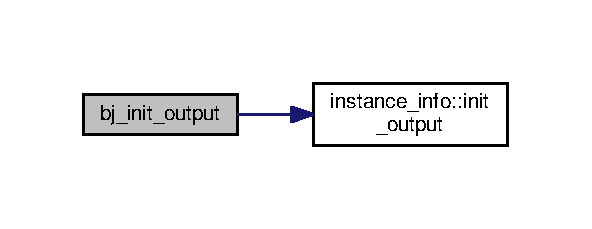
\includegraphics[width=284pt]{dc/d3c/ben__jose_8h_a017fab7c4a46c76367a8810a6a0da452_cgraph}
\end{center}
\end{figure}


\hypertarget{ben__jose_8h_a3f6cb5e5aac2da12b2d475c81909becf}{\index{ben\+\_\+jose.\+h@{ben\+\_\+jose.\+h}!bj\+\_\+solver\+\_\+create@{bj\+\_\+solver\+\_\+create}}
\index{bj\+\_\+solver\+\_\+create@{bj\+\_\+solver\+\_\+create}!ben\+\_\+jose.\+h@{ben\+\_\+jose.\+h}}
\subsubsection[{bj\+\_\+solver\+\_\+create}]{\setlength{\rightskip}{0pt plus 5cm}{\bf bj\+\_\+solver\+\_\+t} bj\+\_\+solver\+\_\+create (
\begin{DoxyParamCaption}
\item[{const char $\ast$}]{bjs\+\_\+dir\+\_\+path}
\end{DoxyParamCaption}
)}}\label{ben__jose_8h_a3f6cb5e5aac2da12b2d475c81909becf}
Create a solver object to solve one or more C\+N\+Fs 
\begin{DoxyParams}{Parameters}
{\em bjs\+\_\+dir\+\_\+path} & A C string that represents the path of the database of C\+N\+Fs. \\
\hline
\end{DoxyParams}
\begin{DoxyReturn}{Returns}
A bj\+\_\+solver\+\_\+t object representing a solver. 
\end{DoxyReturn}
\hypertarget{ben__jose_8h_ae256ffb1a6f33249d57c88ad79c5132b}{\index{ben\+\_\+jose.\+h@{ben\+\_\+jose.\+h}!bj\+\_\+solver\+\_\+release@{bj\+\_\+solver\+\_\+release}}
\index{bj\+\_\+solver\+\_\+release@{bj\+\_\+solver\+\_\+release}!ben\+\_\+jose.\+h@{ben\+\_\+jose.\+h}}
\subsubsection[{bj\+\_\+solver\+\_\+release}]{\setlength{\rightskip}{0pt plus 5cm}void bj\+\_\+solver\+\_\+release (
\begin{DoxyParamCaption}
\item[{{\bf bj\+\_\+solver\+\_\+t}}]{bjs}
\end{DoxyParamCaption}
)}}\label{ben__jose_8h_ae256ffb1a6f33249d57c88ad79c5132b}
Release a solver object created with bj\+\_\+solver\+\_\+create 
\begin{DoxyParams}{Parameters}
{\em bjs} & The solver object to be released. \\
\hline
\end{DoxyParams}
\hypertarget{ben__jose_8h_afeb4622efbaae0a207b9d0a394b860ee}{\index{ben\+\_\+jose.\+h@{ben\+\_\+jose.\+h}!bj\+\_\+set\+\_\+param\+\_\+char@{bj\+\_\+set\+\_\+param\+\_\+char}}
\index{bj\+\_\+set\+\_\+param\+\_\+char@{bj\+\_\+set\+\_\+param\+\_\+char}!ben\+\_\+jose.\+h@{ben\+\_\+jose.\+h}}
\subsubsection[{bj\+\_\+set\+\_\+param\+\_\+char}]{\setlength{\rightskip}{0pt plus 5cm}void bj\+\_\+set\+\_\+param\+\_\+char (
\begin{DoxyParamCaption}
\item[{{\bf bj\+\_\+solver\+\_\+t}}]{bjs, }
\item[{{\bf bj\+\_\+param\+\_\+t}}]{prm, }
\item[{char}]{val}
\end{DoxyParamCaption}
)}}\label{ben__jose_8h_afeb4622efbaae0a207b9d0a394b860ee}
Set an input parameter in the solver 
\begin{DoxyParams}{Parameters}
{\em bjs} & The solver object to be used. \\
\hline
{\em prm} & The parameter. \\
\hline
{\em val} & The value. For boolen values it is 0 (false) or not 0 (true) \\
\hline
\end{DoxyParams}
\hypertarget{ben__jose_8h_ae5e07f54c5d1f3315695876d31bbfc4d}{\index{ben\+\_\+jose.\+h@{ben\+\_\+jose.\+h}!bj\+\_\+get\+\_\+param\+\_\+char@{bj\+\_\+get\+\_\+param\+\_\+char}}
\index{bj\+\_\+get\+\_\+param\+\_\+char@{bj\+\_\+get\+\_\+param\+\_\+char}!ben\+\_\+jose.\+h@{ben\+\_\+jose.\+h}}
\subsubsection[{bj\+\_\+get\+\_\+param\+\_\+char}]{\setlength{\rightskip}{0pt plus 5cm}char bj\+\_\+get\+\_\+param\+\_\+char (
\begin{DoxyParamCaption}
\item[{{\bf bj\+\_\+solver\+\_\+t}}]{bjs, }
\item[{{\bf bj\+\_\+param\+\_\+t}}]{prm}
\end{DoxyParamCaption}
)}}\label{ben__jose_8h_ae5e07f54c5d1f3315695876d31bbfc4d}
Get the value of a previusly set (with bj\+\_\+set\+\_\+param\+\_\+char) input parameter. 
\begin{DoxyParams}{Parameters}
{\em bjs} & The solver object to be used. \\
\hline
{\em prm} & The parameter. \\
\hline
\end{DoxyParams}
\begin{DoxyReturn}{Returns}
The value. For boolen values it is 0 (false) or 1 (true) 
\end{DoxyReturn}
\hypertarget{ben__jose_8h_aacdcf2c366bfd31c06c00cb33a548e9f}{\index{ben\+\_\+jose.\+h@{ben\+\_\+jose.\+h}!bj\+\_\+get\+\_\+database\+\_\+path@{bj\+\_\+get\+\_\+database\+\_\+path}}
\index{bj\+\_\+get\+\_\+database\+\_\+path@{bj\+\_\+get\+\_\+database\+\_\+path}!ben\+\_\+jose.\+h@{ben\+\_\+jose.\+h}}
\subsubsection[{bj\+\_\+get\+\_\+database\+\_\+path}]{\setlength{\rightskip}{0pt plus 5cm}const char$\ast$ bj\+\_\+get\+\_\+database\+\_\+path (
\begin{DoxyParamCaption}
\item[{{\bf bj\+\_\+solver\+\_\+t}}]{bjs}
\end{DoxyParamCaption}
)}}\label{ben__jose_8h_aacdcf2c366bfd31c06c00cb33a548e9f}
Get the value of a previusly set database path (with bj\+\_\+solver\+\_\+create). 
\begin{DoxyParams}{Parameters}
{\em bjs} & The solver object to be used. \\
\hline
\end{DoxyParams}
\begin{DoxyReturn}{Returns}
The database directory path. Do not free the returned pointer. 
\end{DoxyReturn}
\hypertarget{ben__jose_8h_a65eb23939cc4ae39654dbd93343580c8}{\index{ben\+\_\+jose.\+h@{ben\+\_\+jose.\+h}!bj\+\_\+solve\+\_\+file@{bj\+\_\+solve\+\_\+file}}
\index{bj\+\_\+solve\+\_\+file@{bj\+\_\+solve\+\_\+file}!ben\+\_\+jose.\+h@{ben\+\_\+jose.\+h}}
\subsubsection[{bj\+\_\+solve\+\_\+file}]{\setlength{\rightskip}{0pt plus 5cm}{\bf bj\+\_\+satisf\+\_\+val\+\_\+t} bj\+\_\+solve\+\_\+file (
\begin{DoxyParamCaption}
\item[{{\bf bj\+\_\+solver\+\_\+t}}]{bjs, }
\item[{const char $\ast$}]{f\+\_\+path}
\end{DoxyParamCaption}
)}}\label{ben__jose_8h_a65eb23939cc4ae39654dbd93343580c8}
Solve a C\+N\+F given the D\+I\+M\+A\+C\+S formated file path of the C\+N\+F. 
\begin{DoxyParams}{Parameters}
{\em bjs} & The solver object to be used. \\
\hline
{\em f\+\_\+path} & The C\+N\+F file path. It must be in D\+I\+M\+A\+C\+S format. \\
\hline
\end{DoxyParams}
\begin{DoxyReturn}{Returns}
The solving result. 
\end{DoxyReturn}


Here is the call graph for this function\+:\nopagebreak
\begin{figure}[H]
\begin{center}
\leavevmode
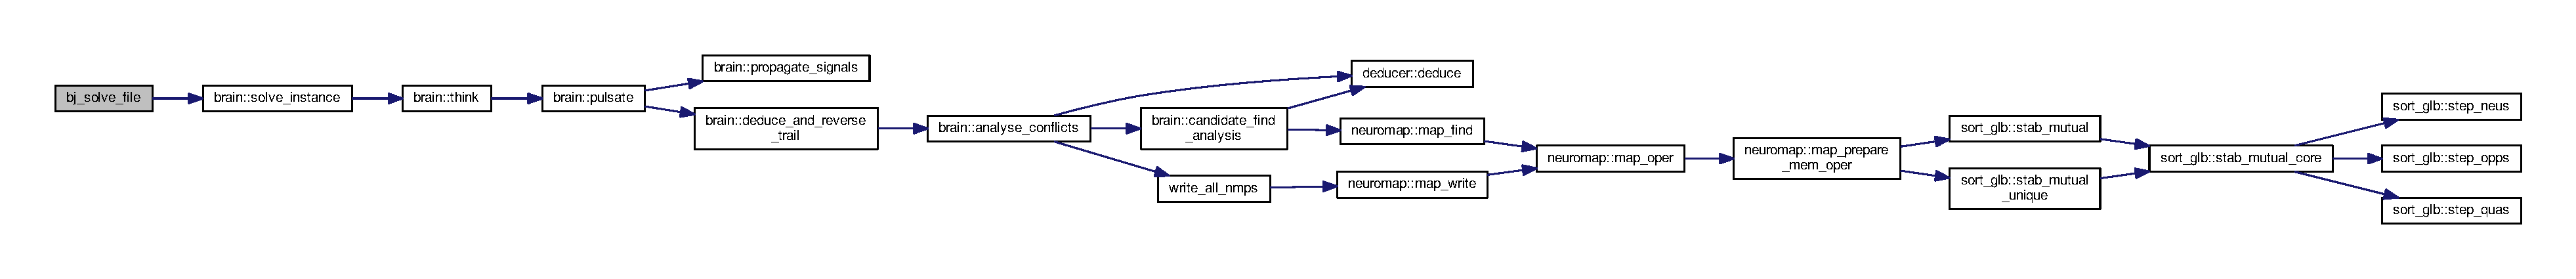
\includegraphics[width=350pt]{dc/d3c/ben__jose_8h_a65eb23939cc4ae39654dbd93343580c8_cgraph}
\end{center}
\end{figure}


\hypertarget{ben__jose_8h_a45eef575a2ca6c6b90e0a1d998f1eb7d}{\index{ben\+\_\+jose.\+h@{ben\+\_\+jose.\+h}!bj\+\_\+solve\+\_\+data@{bj\+\_\+solve\+\_\+data}}
\index{bj\+\_\+solve\+\_\+data@{bj\+\_\+solve\+\_\+data}!ben\+\_\+jose.\+h@{ben\+\_\+jose.\+h}}
\subsubsection[{bj\+\_\+solve\+\_\+data}]{\setlength{\rightskip}{0pt plus 5cm}{\bf bj\+\_\+satisf\+\_\+val\+\_\+t} bj\+\_\+solve\+\_\+data (
\begin{DoxyParamCaption}
\item[{{\bf bj\+\_\+solver\+\_\+t}}]{bjs, }
\item[{long}]{dat\+\_\+sz, }
\item[{const char $\ast$}]{dat}
\end{DoxyParamCaption}
)}}\label{ben__jose_8h_a45eef575a2ca6c6b90e0a1d998f1eb7d}
Solve a C\+N\+F given a D\+I\+M\+A\+C\+S formated C A\+S\+C\+I\+I characters array. 
\begin{DoxyParams}{Parameters}
{\em bjs} & The solver object to be used. \\
\hline
{\em dat\+\_\+sz} & The number of A\+S\+C\+I\+I characters in dat. \\
\hline
{\em dat} & The D\+I\+M\+A\+C\+S formated C A\+S\+C\+I\+I characters array. It can be the exact contents read of a valid D\+I\+M\+A\+C\+S file. \\
\hline
\end{DoxyParams}
\begin{DoxyReturn}{Returns}
The solving result. 
\end{DoxyReturn}


Here is the call graph for this function\+:\nopagebreak
\begin{figure}[H]
\begin{center}
\leavevmode
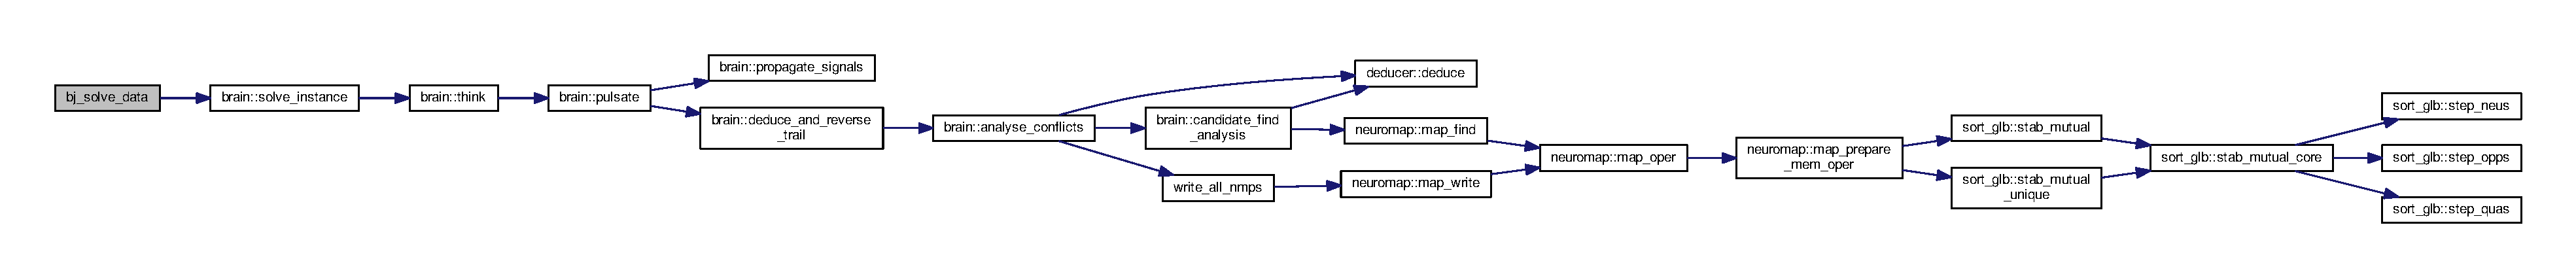
\includegraphics[width=350pt]{dc/d3c/ben__jose_8h_a45eef575a2ca6c6b90e0a1d998f1eb7d_cgraph}
\end{center}
\end{figure}


\hypertarget{ben__jose_8h_a2818f32df95b8d462f49a201ce371142}{\index{ben\+\_\+jose.\+h@{ben\+\_\+jose.\+h}!bj\+\_\+solve\+\_\+literals@{bj\+\_\+solve\+\_\+literals}}
\index{bj\+\_\+solve\+\_\+literals@{bj\+\_\+solve\+\_\+literals}!ben\+\_\+jose.\+h@{ben\+\_\+jose.\+h}}
\subsubsection[{bj\+\_\+solve\+\_\+literals}]{\setlength{\rightskip}{0pt plus 5cm}{\bf bj\+\_\+satisf\+\_\+val\+\_\+t} bj\+\_\+solve\+\_\+literals (
\begin{DoxyParamCaption}
\item[{{\bf bj\+\_\+solver\+\_\+t}}]{bjs, }
\item[{long}]{num\+\_\+vars, }
\item[{long}]{num\+\_\+cls, }
\item[{long}]{lits\+\_\+sz, }
\item[{long $\ast$}]{lits}
\end{DoxyParamCaption}
)}}\label{ben__jose_8h_a2818f32df95b8d462f49a201ce371142}
Solve a C\+N\+F given the D\+I\+M\+A\+C\+S values of a C\+N\+F. 
\begin{DoxyParams}{Parameters}
{\em bjs} & The solver object to be used. \\
\hline
{\em num\+\_\+vars} & The number of variables in used in lits. It is the value as read in a cnf declaration of a D\+I\+M\+A\+C\+S file. \\
\hline
{\em num\+\_\+cls} & The number of clauses found in lits. It is the value as read in a cnf declaration of a D\+I\+M\+A\+C\+S file. \\
\hline
{\em lits\+\_\+sz} & The size of the lits parameter. \\
\hline
{\em lits} & T\+He array containing a set of clauses separated by zeros. Ej\+: \mbox{[}1 2 0 3 4 5 0\mbox{]} representes two clauses\+: \mbox{[}1 2\mbox{]} and \mbox{[}3 4 5\mbox{]}. \\
\hline
\end{DoxyParams}
\begin{DoxyReturn}{Returns}
The solving result. 
\end{DoxyReturn}


Here is the call graph for this function\+:\nopagebreak
\begin{figure}[H]
\begin{center}
\leavevmode
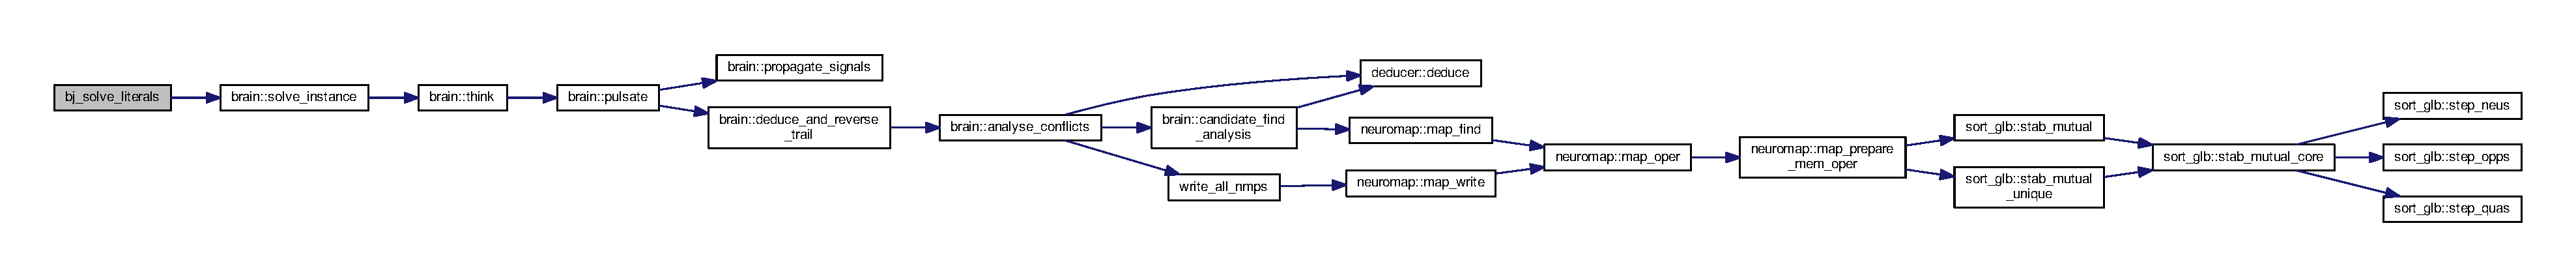
\includegraphics[width=350pt]{dc/d3c/ben__jose_8h_a2818f32df95b8d462f49a201ce371142_cgraph}
\end{center}
\end{figure}


\hypertarget{ben__jose_8h_aef97ca0385d43a4415e6710d07b1dd4d}{\index{ben\+\_\+jose.\+h@{ben\+\_\+jose.\+h}!bj\+\_\+get\+\_\+result@{bj\+\_\+get\+\_\+result}}
\index{bj\+\_\+get\+\_\+result@{bj\+\_\+get\+\_\+result}!ben\+\_\+jose.\+h@{ben\+\_\+jose.\+h}}
\subsubsection[{bj\+\_\+get\+\_\+result}]{\setlength{\rightskip}{0pt plus 5cm}{\bf bj\+\_\+satisf\+\_\+val\+\_\+t} bj\+\_\+get\+\_\+result (
\begin{DoxyParamCaption}
\item[{{\bf bj\+\_\+solver\+\_\+t}}]{bjs}
\end{DoxyParamCaption}
)}}\label{ben__jose_8h_aef97ca0385d43a4415e6710d07b1dd4d}
Get the result of a solving process. A bj\+\_\+solve\+\_\+ function must have been previusly called. 
\begin{DoxyParams}{Parameters}
{\em bjs} & The solver object to be used. \\
\hline
\end{DoxyParams}
\begin{DoxyReturn}{Returns}
The solving result. It has the same value returned by the previusly called bj\+\_\+solve\+\_\+ function. 
\end{DoxyReturn}
\hypertarget{ben__jose_8h_a2685b092d0a891b280bc1895d1deaef1}{\index{ben\+\_\+jose.\+h@{ben\+\_\+jose.\+h}!bj\+\_\+get\+\_\+output@{bj\+\_\+get\+\_\+output}}
\index{bj\+\_\+get\+\_\+output@{bj\+\_\+get\+\_\+output}!ben\+\_\+jose.\+h@{ben\+\_\+jose.\+h}}
\subsubsection[{bj\+\_\+get\+\_\+output}]{\setlength{\rightskip}{0pt plus 5cm}bj\+\_\+output\+\_\+t bj\+\_\+get\+\_\+output (
\begin{DoxyParamCaption}
\item[{{\bf bj\+\_\+solver\+\_\+t}}]{bjs}
\end{DoxyParamCaption}
)}}\label{ben__jose_8h_a2685b092d0a891b280bc1895d1deaef1}
Get all the output a solving process. A bj\+\_\+solve\+\_\+ function must have been previusly called. 
\begin{DoxyParams}{Parameters}
{\em bjs} & The solver object to be used. \\
\hline
\end{DoxyParams}
\begin{DoxyReturn}{Returns}
The solving output. 
\end{DoxyReturn}
\begin{DoxySeeAlso}{See also}
bj\+\_\+output\+\_\+t 
\end{DoxySeeAlso}


Here is the call graph for this function\+:\nopagebreak
\begin{figure}[H]
\begin{center}
\leavevmode
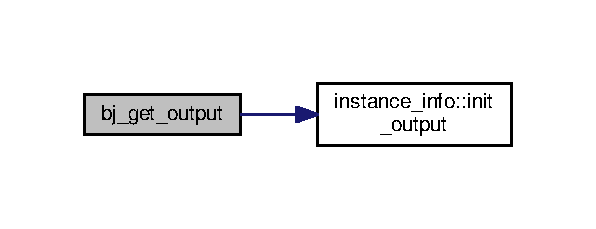
\includegraphics[width=286pt]{dc/d3c/ben__jose_8h_a2685b092d0a891b280bc1895d1deaef1_cgraph}
\end{center}
\end{figure}


\hypertarget{ben__jose_8h_a2cd47bfce4c972f1882857eb7910569d}{\index{ben\+\_\+jose.\+h@{ben\+\_\+jose.\+h}!bj\+\_\+get\+\_\+solve\+\_\+file\+\_\+path@{bj\+\_\+get\+\_\+solve\+\_\+file\+\_\+path}}
\index{bj\+\_\+get\+\_\+solve\+\_\+file\+\_\+path@{bj\+\_\+get\+\_\+solve\+\_\+file\+\_\+path}!ben\+\_\+jose.\+h@{ben\+\_\+jose.\+h}}
\subsubsection[{bj\+\_\+get\+\_\+solve\+\_\+file\+\_\+path}]{\setlength{\rightskip}{0pt plus 5cm}const char$\ast$ bj\+\_\+get\+\_\+solve\+\_\+file\+\_\+path (
\begin{DoxyParamCaption}
\item[{{\bf bj\+\_\+solver\+\_\+t}}]{bjs}
\end{DoxyParamCaption}
)}}\label{ben__jose_8h_a2cd47bfce4c972f1882857eb7910569d}
Returns the value passed to bj\+\_\+solve\+\_\+file. A bj\+\_\+solve\+\_\+ function must have been previusly called. 
\begin{DoxyParams}{Parameters}
{\em bjs} & The solver object to be used. \\
\hline
\end{DoxyParams}
\begin{DoxyReturn}{Returns}
The value passed to bj\+\_\+solve\+\_\+file or null otherwise (other bj\+\_\+solve\+\_\+ function was called). 
\end{DoxyReturn}
\hypertarget{ben__jose_8h_a672cdf8b8774c4224e1cd641f0460705}{\index{ben\+\_\+jose.\+h@{ben\+\_\+jose.\+h}!bj\+\_\+get\+\_\+assig@{bj\+\_\+get\+\_\+assig}}
\index{bj\+\_\+get\+\_\+assig@{bj\+\_\+get\+\_\+assig}!ben\+\_\+jose.\+h@{ben\+\_\+jose.\+h}}
\subsubsection[{bj\+\_\+get\+\_\+assig}]{\setlength{\rightskip}{0pt plus 5cm}const long$\ast$ bj\+\_\+get\+\_\+assig (
\begin{DoxyParamCaption}
\item[{{\bf bj\+\_\+solver\+\_\+t}}]{bjs}
\end{DoxyParamCaption}
)}}\label{ben__jose_8h_a672cdf8b8774c4224e1cd641f0460705}
Get the assignation to variables that satisfies the C\+N\+F. A bj\+\_\+solve\+\_\+ function must have been previusly called. 
\begin{DoxyParams}{Parameters}
{\em bjs} & The solver object to be used. \\
\hline
\end{DoxyParams}
\begin{DoxyReturn}{Returns}
An array (here called 'assig') with the assignation to variables that satisfies the C\+N\+F.
\end{DoxyReturn}
'assig' always ends with a 0.

No memory after that 0 should be accessed.

Let vv = assig\mbox{[}ii\mbox{]}. Then\+:


\begin{DoxyItemize}
\item If vv is positive it means the the variable represented by abs(vv) is assigned true
\item If vv is negative it means the the variable represented by abs(vv) is assigned false
\end{DoxyItemize}

Example\+: \mbox{[}-\/20 4 -\/12 6 9 0\mbox{]}

Means\+:
\begin{DoxyItemize}
\item set var 20 to false
\item set var 4 to true
\item set var 12 to false
\item set var 6 to true
\item set var 9 to true
\end{DoxyItemize}

And that assignation satisfies the whole C\+N\+F (it might have more than 20 variables). \hypertarget{ben__jose_8h_ac3cb476b34f135c0370047bc5ade0058}{\index{ben\+\_\+jose.\+h@{ben\+\_\+jose.\+h}!bj\+\_\+get\+\_\+last\+\_\+proof\+\_\+path@{bj\+\_\+get\+\_\+last\+\_\+proof\+\_\+path}}
\index{bj\+\_\+get\+\_\+last\+\_\+proof\+\_\+path@{bj\+\_\+get\+\_\+last\+\_\+proof\+\_\+path}!ben\+\_\+jose.\+h@{ben\+\_\+jose.\+h}}
\subsubsection[{bj\+\_\+get\+\_\+last\+\_\+proof\+\_\+path}]{\setlength{\rightskip}{0pt plus 5cm}const char$\ast$ bj\+\_\+get\+\_\+last\+\_\+proof\+\_\+path (
\begin{DoxyParamCaption}
\item[{{\bf bj\+\_\+solver\+\_\+t}}]{bjs}
\end{DoxyParamCaption}
)}}\label{ben__jose_8h_ac3cb476b34f135c0370047bc5ade0058}
Returns the last written proof path. A bj\+\_\+solve\+\_\+ function must have been previusly called. 
\begin{DoxyParams}{Parameters}
{\em bjs} & The solver object to be used. \\
\hline
\end{DoxyParams}
\begin{DoxyReturn}{Returns}
The path to the last written G\+S\+O\+N proof file.
\end{DoxyReturn}
N\+U\+L\+L is returned if the parameter bjp\+\_\+write\+\_\+proofs was not used before calling a bj\+\_\+solve\+\_\+ function. \hypertarget{ben__jose_8h_abf18e6ff43cc5a12b15d6317da5357ef}{\index{ben\+\_\+jose.\+h@{ben\+\_\+jose.\+h}!bj\+\_\+get\+\_\+error\+\_\+stack\+\_\+str@{bj\+\_\+get\+\_\+error\+\_\+stack\+\_\+str}}
\index{bj\+\_\+get\+\_\+error\+\_\+stack\+\_\+str@{bj\+\_\+get\+\_\+error\+\_\+stack\+\_\+str}!ben\+\_\+jose.\+h@{ben\+\_\+jose.\+h}}
\subsubsection[{bj\+\_\+get\+\_\+error\+\_\+stack\+\_\+str}]{\setlength{\rightskip}{0pt plus 5cm}const char$\ast$ bj\+\_\+get\+\_\+error\+\_\+stack\+\_\+str (
\begin{DoxyParamCaption}
\item[{{\bf bj\+\_\+solver\+\_\+t}}]{bjs}
\end{DoxyParamCaption}
)}}\label{ben__jose_8h_abf18e6ff43cc5a12b15d6317da5357ef}
Get the stack when the error ocurred. A bj\+\_\+solve\+\_\+ function must have been previusly called. 
\begin{DoxyParams}{Parameters}
{\em bjs} & The solver object to be used. \\
\hline
\end{DoxyParams}
\begin{DoxyReturn}{Returns}
The stack when the error ocurred.
\end{DoxyReturn}
Funtion for debugging purposes. Only returns a valid value if an error has ocurred during solving. \hypertarget{ben__jose_8h_aa74202918cc8ec8e05d541a9fa04251f}{\index{ben\+\_\+jose.\+h@{ben\+\_\+jose.\+h}!bj\+\_\+get\+\_\+error\+\_\+assert\+\_\+str@{bj\+\_\+get\+\_\+error\+\_\+assert\+\_\+str}}
\index{bj\+\_\+get\+\_\+error\+\_\+assert\+\_\+str@{bj\+\_\+get\+\_\+error\+\_\+assert\+\_\+str}!ben\+\_\+jose.\+h@{ben\+\_\+jose.\+h}}
\subsubsection[{bj\+\_\+get\+\_\+error\+\_\+assert\+\_\+str}]{\setlength{\rightskip}{0pt plus 5cm}const char$\ast$ bj\+\_\+get\+\_\+error\+\_\+assert\+\_\+str (
\begin{DoxyParamCaption}
\item[{{\bf bj\+\_\+solver\+\_\+t}}]{bjs}
\end{DoxyParamCaption}
)}}\label{ben__jose_8h_aa74202918cc8ec8e05d541a9fa04251f}
Get the assert that failed. A bj\+\_\+solve\+\_\+ function must have been previusly called. 
\begin{DoxyParams}{Parameters}
{\em bjs} & The solver object to be used. \\
\hline
\end{DoxyParams}
\begin{DoxyReturn}{Returns}
The assert that failed.
\end{DoxyReturn}
Funtion for debugging purposes. Only returns a valid value if an assert has failed. \hypertarget{ben__jose_8h_a09f75c893eb86496a7fa1eba093b9d67}{\index{ben\+\_\+jose.\+h@{ben\+\_\+jose.\+h}!bj\+\_\+get\+\_\+result\+\_\+titles\+\_\+string@{bj\+\_\+get\+\_\+result\+\_\+titles\+\_\+string}}
\index{bj\+\_\+get\+\_\+result\+\_\+titles\+\_\+string@{bj\+\_\+get\+\_\+result\+\_\+titles\+\_\+string}!ben\+\_\+jose.\+h@{ben\+\_\+jose.\+h}}
\subsubsection[{bj\+\_\+get\+\_\+result\+\_\+titles\+\_\+string}]{\setlength{\rightskip}{0pt plus 5cm}const char$\ast$ bj\+\_\+get\+\_\+result\+\_\+titles\+\_\+string (
\begin{DoxyParamCaption}
\item[{{\bf bj\+\_\+solver\+\_\+t}}]{bjs}
\end{DoxyParamCaption}
)}}\label{ben__jose_8h_a09f75c893eb86496a7fa1eba093b9d67}
Get a string with the titles of a result string fields. 
\begin{DoxyParams}{Parameters}
{\em bjs} & The solver object to be used. \\
\hline
\end{DoxyParams}
\begin{DoxyReturn}{Returns}
A string with the titles of a result string fields.
\end{DoxyReturn}
Funtion for testing purposes. \hypertarget{ben__jose_8h_aef3c645a9b041d6f7fd7aa720d255308}{\index{ben\+\_\+jose.\+h@{ben\+\_\+jose.\+h}!bj\+\_\+get\+\_\+result\+\_\+string@{bj\+\_\+get\+\_\+result\+\_\+string}}
\index{bj\+\_\+get\+\_\+result\+\_\+string@{bj\+\_\+get\+\_\+result\+\_\+string}!ben\+\_\+jose.\+h@{ben\+\_\+jose.\+h}}
\subsubsection[{bj\+\_\+get\+\_\+result\+\_\+string}]{\setlength{\rightskip}{0pt plus 5cm}const char$\ast$ bj\+\_\+get\+\_\+result\+\_\+string (
\begin{DoxyParamCaption}
\item[{{\bf bj\+\_\+solver\+\_\+t}}]{bjs}
\end{DoxyParamCaption}
)}}\label{ben__jose_8h_aef3c645a9b041d6f7fd7aa720d255308}
Get a string with the result string. A bj\+\_\+solve\+\_\+ function must have been previusly called. 
\begin{DoxyParams}{Parameters}
{\em bjs} & The solver object to be used. \\
\hline
\end{DoxyParams}
\begin{DoxyReturn}{Returns}
A string with the result string.
\end{DoxyReturn}
Funtion for testing purposes. It contains a concatenation of the string representation of some fields obtained otherwise with the bj\+\_\+get\+\_\+output funtion. \hypertarget{ben__jose_8h_ac23228b810b4eadd052ee3dcc193a0a5}{\index{ben\+\_\+jose.\+h@{ben\+\_\+jose.\+h}!bj\+\_\+parse\+\_\+result\+\_\+string@{bj\+\_\+parse\+\_\+result\+\_\+string}}
\index{bj\+\_\+parse\+\_\+result\+\_\+string@{bj\+\_\+parse\+\_\+result\+\_\+string}!ben\+\_\+jose.\+h@{ben\+\_\+jose.\+h}}
\subsubsection[{bj\+\_\+parse\+\_\+result\+\_\+string}]{\setlength{\rightskip}{0pt plus 5cm}void bj\+\_\+parse\+\_\+result\+\_\+string (
\begin{DoxyParamCaption}
\item[{{\bf bj\+\_\+solver\+\_\+t}}]{bjs, }
\item[{const char $\ast$}]{rslt\+\_\+str}
\end{DoxyParamCaption}
)}}\label{ben__jose_8h_ac23228b810b4eadd052ee3dcc193a0a5}
Sets internal values in the solver with a result string previusly returned by bj\+\_\+get\+\_\+result\+\_\+string. 
\begin{DoxyParams}{Parameters}
{\em bjs} & The solver object to be used. \\
\hline
{\em rslt\+\_\+str} & A string with the result string.\\
\hline
\end{DoxyParams}
Funtion for testing purposes. It sets internal values in the solver so that a call to bj\+\_\+get\+\_\+output will return the parsed values. \hypertarget{ben__jose_8h_a62d44e173c8c8d19dae9c88696649127}{\index{ben\+\_\+jose.\+h@{ben\+\_\+jose.\+h}!bj\+\_\+restart@{bj\+\_\+restart}}
\index{bj\+\_\+restart@{bj\+\_\+restart}!ben\+\_\+jose.\+h@{ben\+\_\+jose.\+h}}
\subsubsection[{bj\+\_\+restart}]{\setlength{\rightskip}{0pt plus 5cm}void bj\+\_\+restart (
\begin{DoxyParamCaption}
\item[{{\bf bj\+\_\+solver\+\_\+t}}]{bjs}
\end{DoxyParamCaption}
)}}\label{ben__jose_8h_a62d44e173c8c8d19dae9c88696649127}
Resets all internal values in the solver. 
\begin{DoxyParams}{Parameters}
{\em bjs} & The solver object to be used. \\
\hline
\end{DoxyParams}
\hypertarget{ben__jose_8h_ac7ff7cedad8c30e85232f52cb1c6e716}{\index{ben\+\_\+jose.\+h@{ben\+\_\+jose.\+h}!bj\+\_\+print\+\_\+paths@{bj\+\_\+print\+\_\+paths}}
\index{bj\+\_\+print\+\_\+paths@{bj\+\_\+print\+\_\+paths}!ben\+\_\+jose.\+h@{ben\+\_\+jose.\+h}}
\subsubsection[{bj\+\_\+print\+\_\+paths}]{\setlength{\rightskip}{0pt plus 5cm}void bj\+\_\+print\+\_\+paths (
\begin{DoxyParamCaption}
\item[{{\bf bj\+\_\+solver\+\_\+t}}]{bjs}
\end{DoxyParamCaption}
)}}\label{ben__jose_8h_ac7ff7cedad8c30e85232f52cb1c6e716}
Prints all paths used by the solver. 
\begin{DoxyParams}{Parameters}
{\em bjs} & The solver object to be used. \\
\hline
\end{DoxyParams}
\hypertarget{ben__jose_8h_ab6303f60ba14cddd8b534b40830df31d}{\index{ben\+\_\+jose.\+h@{ben\+\_\+jose.\+h}!bj\+\_\+error\+\_\+str@{bj\+\_\+error\+\_\+str}}
\index{bj\+\_\+error\+\_\+str@{bj\+\_\+error\+\_\+str}!ben\+\_\+jose.\+h@{ben\+\_\+jose.\+h}}
\subsubsection[{bj\+\_\+error\+\_\+str}]{\setlength{\rightskip}{0pt plus 5cm}const char$\ast$ bj\+\_\+error\+\_\+str (
\begin{DoxyParamCaption}
\item[{{\bf bj\+\_\+error\+\_\+t}}]{bje}
\end{DoxyParamCaption}
)}}\label{ben__jose_8h_ab6303f60ba14cddd8b534b40830df31d}
Gets a string representing the error. A bj\+\_\+solve\+\_\+ function must have been previusly called. 
\begin{DoxyParams}{Parameters}
{\em bjs} & The solver object to be used. \\
\hline
\end{DoxyParams}
\begin{DoxyReturn}{Returns}
A string representing the error. 
\end{DoxyReturn}

\hypertarget{brain_8h}{}\section{/home/jose/devel/ben-\/jose/src/library/brain/brain.h File Reference}
\label{brain_8h}\index{/home/jose/devel/ben-\/jose/src/library/brain/brain.\+h@{/home/jose/devel/ben-\/jose/src/library/brain/brain.\+h}}


Declarations of classes and that implement the solver\textquotesingle{}s core functionality.  


{\ttfamily \#include \char`\"{}stack\+\_\+trace.\+h\char`\"{}}\\*
{\ttfamily \#include \char`\"{}tools.\+h\char`\"{}}\\*
{\ttfamily \#include \char`\"{}binder.\+h\char`\"{}}\\*
{\ttfamily \#include \char`\"{}ben\+\_\+jose.\+h\char`\"{}}\\*
{\ttfamily \#include \char`\"{}instance\+\_\+info.\+h\char`\"{}}\\*
{\ttfamily \#include \char`\"{}sortor.\+h\char`\"{}}\\*
{\ttfamily \#include \char`\"{}dbg\+\_\+config.\+h\char`\"{}}\\*
{\ttfamily \#include \char`\"{}dbg\+\_\+prt.\+h\char`\"{}}\\*
Include dependency graph for brain.\+h\+:
\nopagebreak
\begin{figure}[H]
\begin{center}
\leavevmode
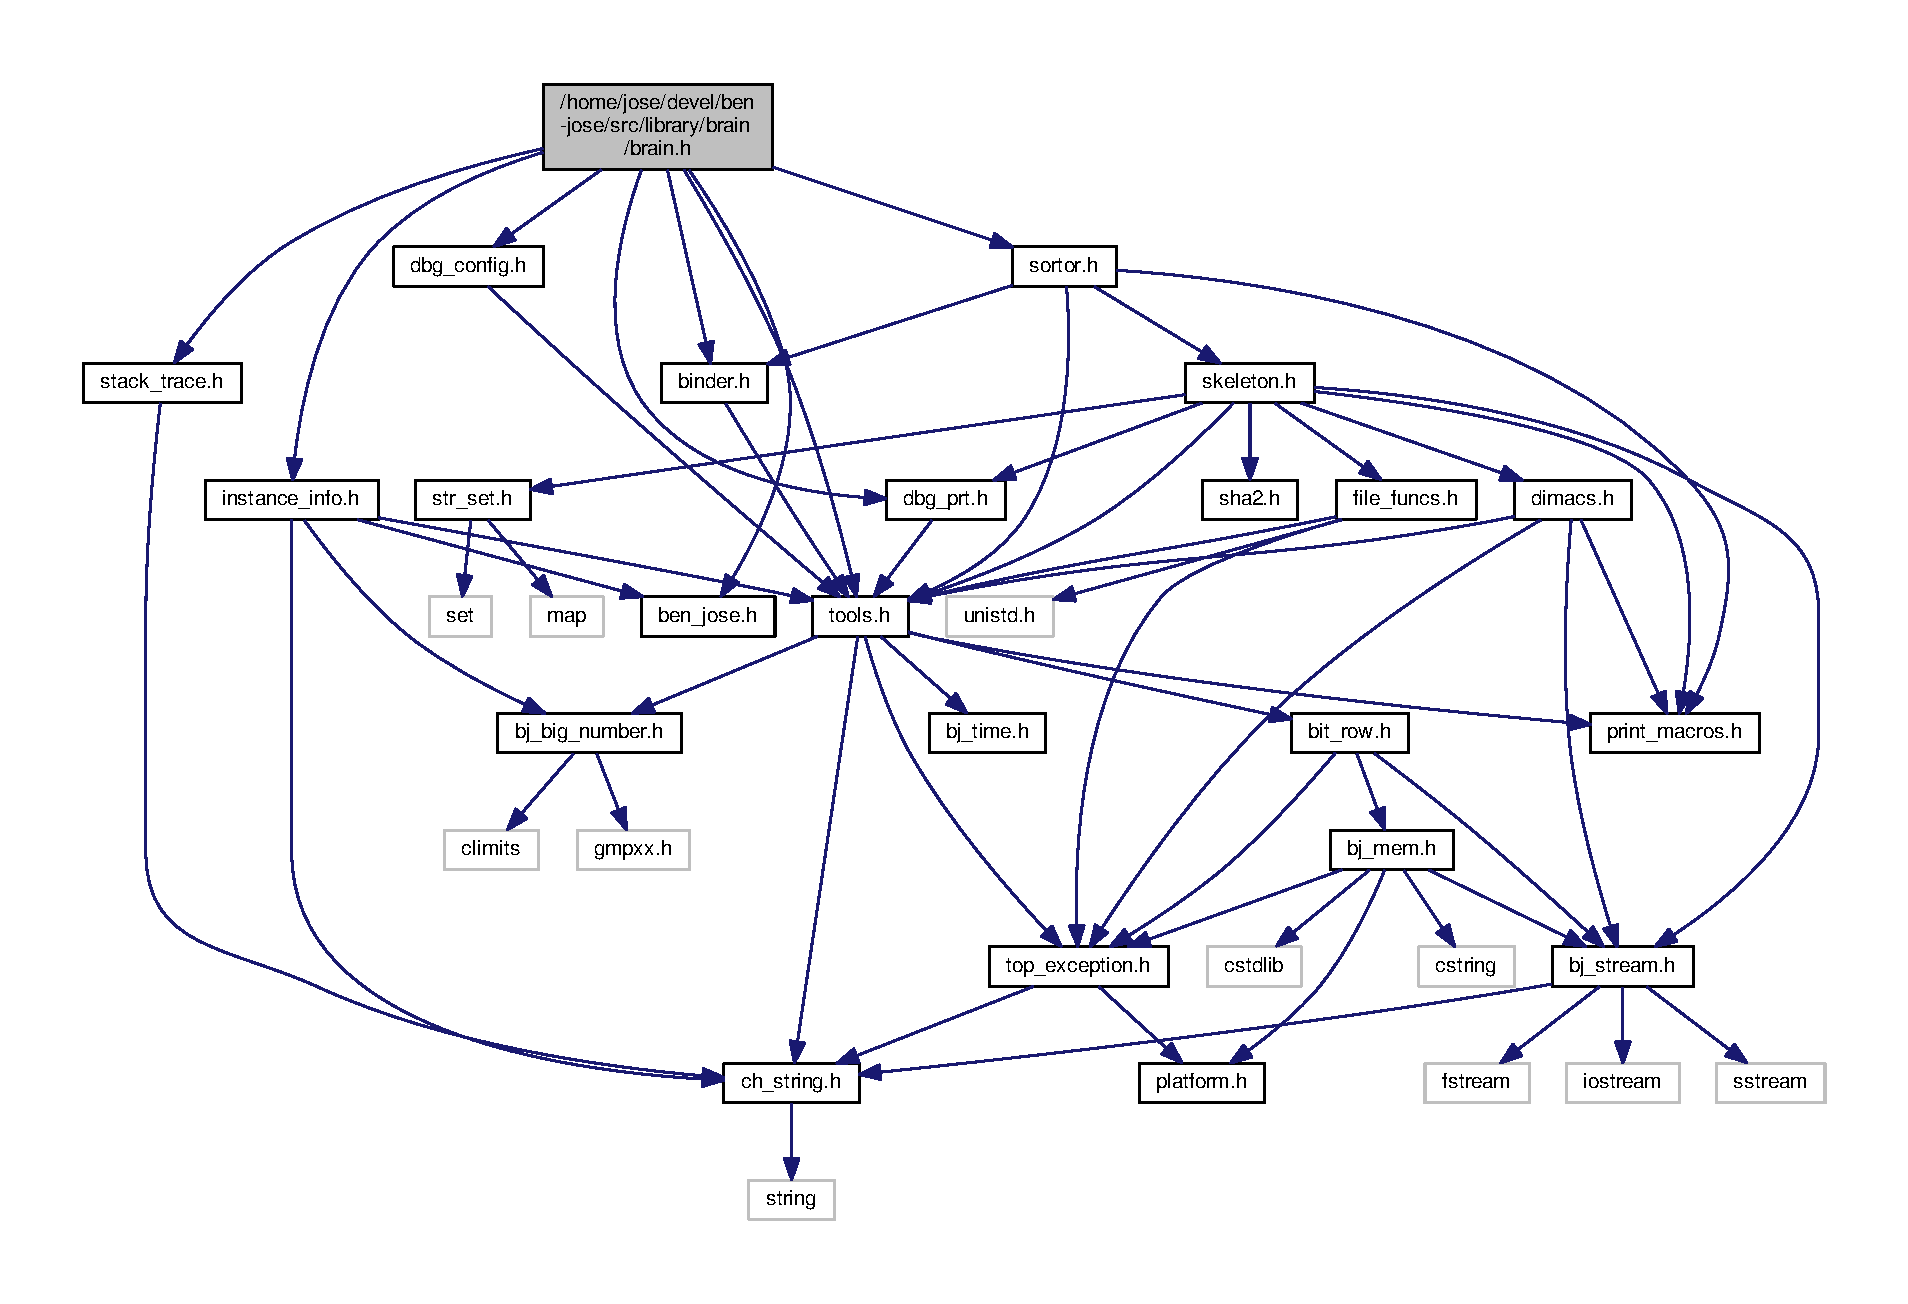
\includegraphics[width=350pt]{dc/d30/brain_8h__incl}
\end{center}
\end{figure}
This graph shows which files directly or indirectly include this file\+:
\nopagebreak
\begin{figure}[H]
\begin{center}
\leavevmode
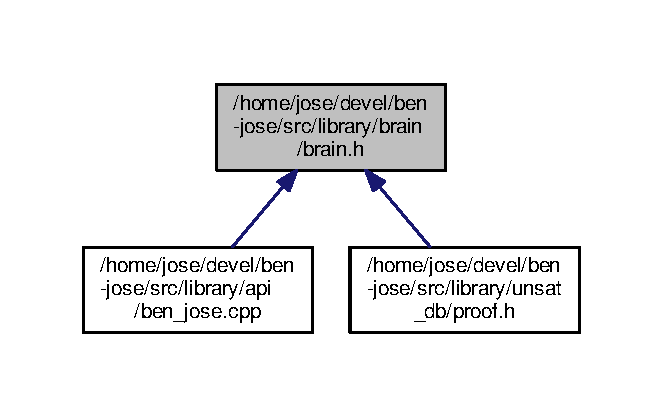
\includegraphics[width=318pt]{da/d98/brain_8h__dep__incl}
\end{center}
\end{figure}
\subsection*{Classes}
\begin{DoxyCompactItemize}
\item 
class \hyperlink{classquanton}{quanton}
\begin{DoxyCompactList}\small\item\em Class for C\+NF variables (each variable has a positon and a negaton). \end{DoxyCompactList}\item 
class \hyperlink{classcoloring}{coloring}
\begin{DoxyCompactList}\small\item\em The initial and final state for an stabilization is a coloring. \end{DoxyCompactList}\item 
class \hyperlink{classneuron}{neuron}
\begin{DoxyCompactList}\small\item\em Class for C\+NF clause behavior. So there is one neuron per clause. \end{DoxyCompactList}\item 
class \hyperlink{classprop__signal}{prop\+\_\+signal}
\begin{DoxyCompactList}\small\item\em Class for representing B\+CP propagation data. \end{DoxyCompactList}\item 
class \hyperlink{classdeduction}{deduction}
\begin{DoxyCompactList}\small\item\em Class that holds the result of analyzing (doing resolution) of a conflict. \end{DoxyCompactList}\item 
class \hyperlink{classneuromap}{neuromap}
\begin{DoxyCompactList}\small\item\em A neuromap is a C\+NF sub-\/formula. \end{DoxyCompactList}\item 
class \hyperlink{classdeducer}{deducer}
\begin{DoxyCompactList}\small\item\em Class that holds the data used to analyze a conflict. \end{DoxyCompactList}\item 
class \hyperlink{classleveldat}{leveldat}
\begin{DoxyCompactList}\small\item\em Class that holds the data of a level. \end{DoxyCompactList}\item 
class \hyperlink{classbrain}{brain}
\begin{DoxyCompactList}\small\item\em Class that holds all data used to solve a particular C\+NF instance. \end{DoxyCompactList}\end{DoxyCompactItemize}
\subsection*{Functions}
\begin{DoxyCompactItemize}
\item 
void \hyperlink{brain_8h_a14f74143760dde7c17a99c26c736c198}{write\+\_\+all\+\_\+nmps} (row\+\_\+neuromap\+\_\+t \&to\+\_\+wrt)
\begin{DoxyCompactList}\small\item\em Writes all \hyperlink{classneuromap}{neuromap} s (candidates) that need writing. \end{DoxyCompactList}\end{DoxyCompactItemize}


\subsection{Detailed Description}
Declarations of classes and that implement the solver\textquotesingle{}s core functionality. 



\subsection{Function Documentation}
\index{brain.\+h@{brain.\+h}!write\+\_\+all\+\_\+nmps@{write\+\_\+all\+\_\+nmps}}
\index{write\+\_\+all\+\_\+nmps@{write\+\_\+all\+\_\+nmps}!brain.\+h@{brain.\+h}}
\subsubsection[{\texorpdfstring{write\+\_\+all\+\_\+nmps(row\+\_\+neuromap\+\_\+t \&to\+\_\+wrt)}{write_all_nmps(row_neuromap_t &to_wrt)}}]{\setlength{\rightskip}{0pt plus 5cm}void brain\+::write\+\_\+all\+\_\+nmps (
\begin{DoxyParamCaption}
\item[{row$<$ {\bf neuromap} $\ast$ $>$ \&}]{to\+\_\+wrt}
\end{DoxyParamCaption}
)}\hypertarget{brain_8h_a14f74143760dde7c17a99c26c736c198}{}\label{brain_8h_a14f74143760dde7c17a99c26c736c198}


Writes all \hyperlink{classneuromap}{neuromap} s (candidates) that need writing. 

\begin{DoxySeeAlso}{See also}
\hyperlink{macro__algorithm__ben__jose_8cpp}{macro\+\_\+algorithm\+\_\+ben\+\_\+jose.\+cpp} 
\end{DoxySeeAlso}


Here is the call graph for this function\+:
\nopagebreak
\begin{figure}[H]
\begin{center}
\leavevmode
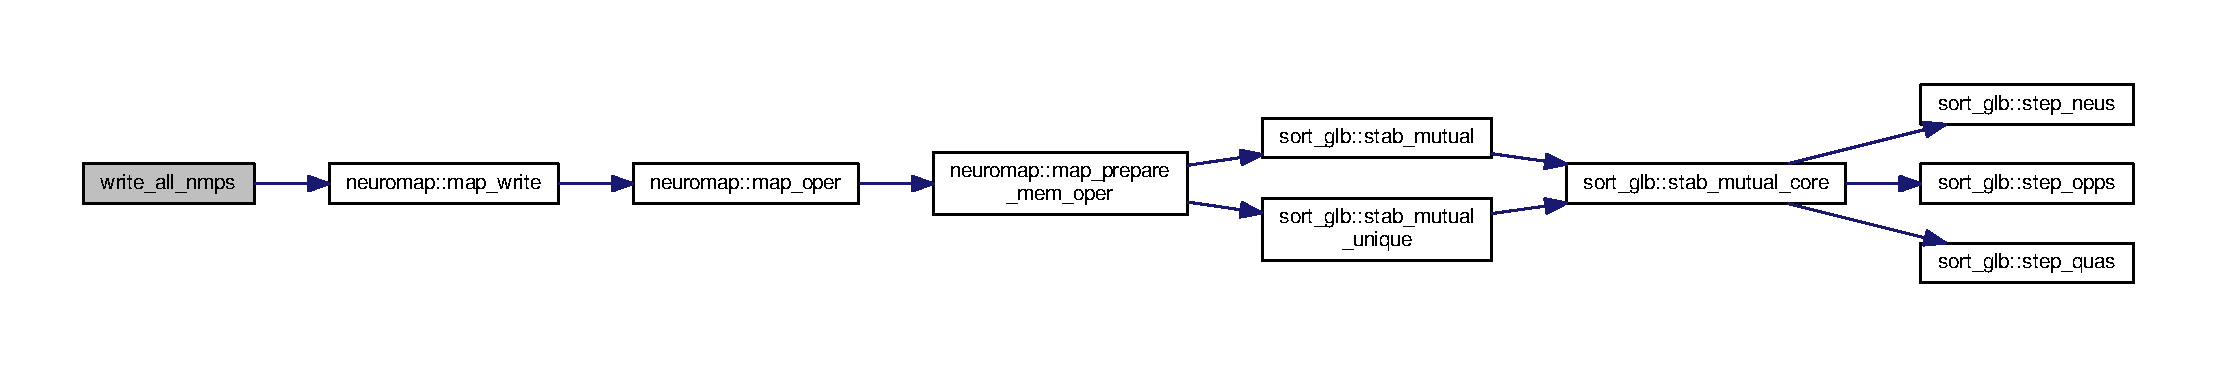
\includegraphics[width=350pt]{db/d3c/brain_8h_a14f74143760dde7c17a99c26c736c198_cgraph}
\end{center}
\end{figure}




Here is the caller graph for this function\+:
\nopagebreak
\begin{figure}[H]
\begin{center}
\leavevmode
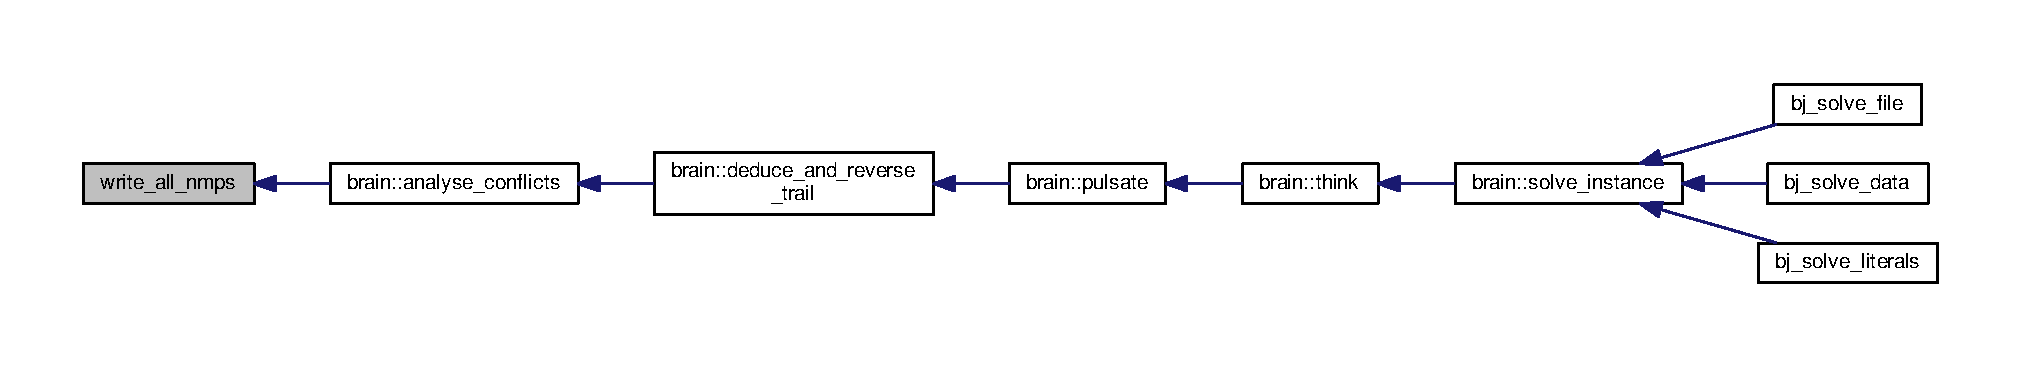
\includegraphics[width=350pt]{db/d3c/brain_8h_a14f74143760dde7c17a99c26c736c198_icgraph}
\end{center}
\end{figure}



\hypertarget{macro__algorithm__ben__jose_8cpp}{}\section{/home/jose/devel/ben-\/jose/src/programs/macro\+\_\+ben\+\_\+jose/macro\+\_\+algorithm\+\_\+ben\+\_\+jose.cpp File Reference}
\label{macro__algorithm__ben__jose_8cpp}\index{/home/jose/devel/ben-\/jose/src/programs/macro\+\_\+ben\+\_\+jose/macro\+\_\+algorithm\+\_\+ben\+\_\+jose.\+cpp@{/home/jose/devel/ben-\/jose/src/programs/macro\+\_\+ben\+\_\+jose/macro\+\_\+algorithm\+\_\+ben\+\_\+jose.\+cpp}}


This is a documentation file to help understand the innerworking of the library. It is not compiled.  


\subsection*{Macros}
\begin{DoxyCompactItemize}
\item 
\#define \hyperlink{macro__algorithm__ben__jose_8cpp_a6c1ce86bc2c830291e5c4e027c26c90f}{T\+H\+I\+S\+\_\+\+C\+O\+D\+E\+\_\+\+I\+S\+\_\+\+N\+O\+T\+\_\+\+C\+O\+M\+P\+I\+L\+ED}\hypertarget{macro__algorithm__ben__jose_8cpp_a6c1ce86bc2c830291e5c4e027c26c90f}{}\label{macro__algorithm__ben__jose_8cpp_a6c1ce86bc2c830291e5c4e027c26c90f}

\begin{DoxyCompactList}\small\item\em \mbox{[}macro\+\_\+bj\+\_\+id\mbox{]} \end{DoxyCompactList}\end{DoxyCompactItemize}


\subsection{Detailed Description}
This is a documentation file to help understand the innerworking of the library. It is not compiled. 

It is an outline of the functions that get called during the solving of a S\+AT instance when the user of the library uses one of the three presentations of the ben-\/jose A\+PI top solve instances\+:

\begin{DoxySeeAlso}{See also}
\hyperlink{ben__jose_8h_a65eb23939cc4ae39654dbd93343580c8}{bj\+\_\+solve\+\_\+file} 

\hyperlink{ben__jose_8h_a45eef575a2ca6c6b90e0a1d998f1eb7d}{bj\+\_\+solve\+\_\+data} 

\hyperlink{ben__jose_8h_a2818f32df95b8d462f49a201ce371142}{bj\+\_\+solve\+\_\+literals}
\end{DoxySeeAlso}
This file is not compiled it is just to help in the understanding of the inner-\/works of the library, and to help the interested programmer to get familiar with the backbone functions of the library.

The following are its contents\+:


\begin{DoxyCodeInclude}
\textcolor{preprocessor}{#define THIS\_CODE\_IS\_NOT\_COMPILED}

\textcolor{keywordtype}{void}
\hyperlink{classbrain_a2daa8c1c03eea62a51a359470bb64cc7}{brain::solve\_instance}()\{
    \textcolor{comment}{// init all brain data with any of:}
    \textcolor{comment}{//      a DIMACS file}
    \textcolor{comment}{//      a byte array (the chars in a DIMACS file)}
    \textcolor{comment}{//      a literals array (long ints represent literals}
    \textcolor{comment}{//          and a 0 separates clauses)}
    load\_instance(); 
    \hyperlink{classbrain_a8524441f8b863aec8fe2cc9c3ad2d21a}{think}();
\}

\textcolor{keywordtype}{void} 
\hyperlink{classbrain_a8524441f8b863aec8fe2cc9c3ad2d21a}{brain::think}()\{
    \textcolor{keywordflow}{while}(o\_info.bjo\_result == \hyperlink{ben__jose_8h_ga9aba221730ab694a549d25ee1aa28c69ad8dafe2640a5e989a73880526a853663}{bjr\_unknown\_satisf})\{
        \hyperlink{classbrain_a9728a44b4e7b71ddb4a47bb25af05612}{pulsate}();
    \}
\}

\textcolor{keywordtype}{void}
\hyperlink{classbrain_a9728a44b4e7b71ddb4a47bb25af05612}{brain::pulsate}()\{
    \hyperlink{classbrain_a28eeaf513dd81fcb3dcb21fb37f58ccb}{propagate\_signals}();
    \textcolor{keywordflow}{if}(found\_conflict())\{
        \hyperlink{classbrain_a8d880c7f0e91a5dbb2cedaefdb704153}{deduce\_and\_reverse\_trail}();
    \} \textcolor{keywordflow}{else}\{
        choose\_quanton();
        start\_propagation();
    \}
\}

\textcolor{keywordtype}{void}
\hyperlink{classbrain_a8d880c7f0e91a5dbb2cedaefdb704153}{brain::deduce\_and\_reverse\_trail}()\{
    \hyperlink{classdeduction}{deduction}& dct = br\_pulse\_deduc;
    reason& rsn = dct.dt\_rsn;
    
    dct.reset\_deduction();
    
    \hyperlink{classbrain_adec5742918fedd1636a6152502bd409c}{analyse\_conflicts}(br\_all\_conflicts\_found, dct);
    reverse\_with(rsn);
\}

\textcolor{keywordtype}{void}
\hyperlink{classbrain_adec5742918fedd1636a6152502bd409c}{brain::analyse\_conflicts}()\{
    \hyperlink{classdeduction}{deduction}& dct = br\_pulse\_deduc;
    \hyperlink{classdeducer}{deducer}& ddc = br\_dedcer;
    
    dct.reset\_deduction();
    ddc.\hyperlink{classdeducer_a7db42a9dfc25ed6ed6747faea2c90961}{deduce}(dct); \textcolor{comment}{// good old conflict analysis. }
    \textcolor{comment}{//it finds a reason (clause) for a conflict}
    
    \hyperlink{classbrain_a16dcda6892686c581ca095f51e6a9def}{candidate\_find\_analysis}(ddc, dct); \textcolor{comment}{// try to go further by }
    \textcolor{comment}{// finding unsat sub-formulas}

    row\_neuromap\_t& to\_wrt = dct.dt\_all\_to\_wrt;
    \hyperlink{brain_8h_a14f74143760dde7c17a99c26c736c198}{write\_all\_nmps}(to\_wrt);
    
\}

\textcolor{keywordtype}{void}
\hyperlink{brain_8h_a14f74143760dde7c17a99c26c736c198}{brain::write\_all\_nmps}(row<neuromap*>& to\_wrt)\{
    \textcolor{keywordflow}{for}(\textcolor{keywordtype}{int} aa = 0; aa < to\_wrt.size(); aa++)\{
        \hyperlink{classneuromap}{neuromap}& nmp = *(to\_wrt[aa]);
        nmp.\hyperlink{classneuromap_adb0c3a4698866c919272f9b4ba5998fd}{map\_write}();
    \}
\}

\textcolor{keywordtype}{void}
\hyperlink{classbrain_a16dcda6892686c581ca095f51e6a9def}{brain::candidate\_find\_analysis}(\hyperlink{classdeducer}{deducer}& dedcer, 
      \hyperlink{classdeduction}{deduction}& dct)\{
    \hyperlink{classneuromap}{neuromap}* out\_nmp = NULL\_PT;
    \textcolor{keywordflow}{for}(\textcolor{keywordtype}{long} aa = br\_candidate\_nmp\_lvs.last\_idx(); aa >= 0; aa--)\{
        out\_nmp = br\_candidate\_nmp\_lvs[aa];
        \textcolor{keywordflow}{if}(! out\_nmp->\hyperlink{classneuromap_a5da738c0ecb7ba74a4fc435ca33b1fcb}{map\_find}())\{
            \textcolor{keywordflow}{break};
        \}
        dct.reset\_deduction();
        dedcer.\hyperlink{classdeducer_a7db42a9dfc25ed6ed6747faea2c90961}{deduce}(dct);
    \}
\}

\textcolor{keywordtype}{bool}
\hyperlink{classneuromap_a5da738c0ecb7ba74a4fc435ca33b1fcb}{neuromap::map\_find}()\{
    \textcolor{keywordflow}{return} map\_oper(mo\_find);
\}

\textcolor{keywordtype}{bool}
\hyperlink{classneuromap_adb0c3a4698866c919272f9b4ba5998fd}{neuromap::map\_write}()\{
    \textcolor{keywordflow}{return} map\_oper(mo\_save);
\}

\textcolor{keywordtype}{bool}
\hyperlink{classneuromap_a5ad7c9c245129fc8a162742c11d4e972}{neuromap::map\_oper}(mem\_op\_t mm)\{
    \textcolor{comment}{// prepare the neuromap: stabilize it to find it's BCFF.}
    \textcolor{keywordtype}{bool} prep\_ok = map\_prepare\_mem\_oper(mm);
    \textcolor{keywordflow}{if}(! prep\_ok)\{
        \textcolor{keywordflow}{return} \textcolor{keyword}{false};
    \}
    \hyperlink{classbrain}{brain}& brn = get\_brn();
    \hyperlink{classskeleton__glb}{skeleton\_glb}& skg = brn.get\_skeleton();
    
    \hyperlink{classcanon__cnf}{canon\_cnf}& tmp\_tauto\_cnf = brn.br\_tmp\_wrt\_tauto\_cnf; \textcolor{comment}{// the unsat BCFF }
    \hyperlink{classcanon__cnf}{canon\_cnf}& tmp\_diff\_cnf = brn.br\_tmp\_wrt\_diff\_cnf; \textcolor{comment}{// the diff between tauto and guide.}
    \hyperlink{classcanon__cnf}{canon\_cnf}& tmp\_guide\_cnf = brn.br\_tmp\_wrt\_guide\_cnf; \textcolor{comment}{// the guide of tauto}
    
    \textcolor{keywordflow}{if}(mm == mo\_find)\{
        \hyperlink{classinstance__info}{instance\_info}& iinfo = brn.get\_my\_inst();
        row\_neuron\_t& all\_found = na\_found\_col.co\_neus;
        
        \textcolor{comment}{// find this neuromap in the skeleton:}
        tmp\_diff\_cnf.first\_vnt\_i\_super\_of(skg, all\_found, &iinfo); 
    \} \textcolor{keywordflow}{else} \{
        ch\_string& tau\_pth = na\_tauto\_pth;

        \textcolor{comment}{// write all relevant cnfs of this neuromap in the skeleton:}
        tmp\_tauto\_cnf.save\_cnf(skg, tau\_pth);
        tmp\_diff\_cnf.save\_cnf(skg, tau\_pth);
        tmp\_guide\_cnf.save\_cnf(skg, tau\_pth);
    \}
\}

\textcolor{keywordtype}{bool}
\hyperlink{classneuromap_a9c0e877474e2d17cf8b9da564de8b8c3}{neuromap::map\_prepare\_mem\_oper}(mem\_op\_t mm)\{
    \hyperlink{classbrain}{brain}& brn = get\_brn();
    
    brn.all\_mutual\_init(); \textcolor{comment}{// init all stab aux params}
    
    \textcolor{comment}{// final stab of the guide}
    \hyperlink{classsort__glb}{sort\_glb}& guide\_ne\_srg = brn.br\_guide\_neus\_srg;
    \hyperlink{classsort__glb}{sort\_glb}& guide\_qu\_srg = brn.br\_guide\_quas\_srg;

    \textcolor{comment}{// init sort\_glb info and do some stab.}
    \textcolor{keywordflow}{if}(! has\_stab\_guide())\{
        map\_set\_stab\_guide();
    \} \textcolor{keywordflow}{else} \{
        guide\_col.load\_colors\_into(guide\_ne\_srg, guide\_qu\_srg, dbg\_call\_1, \textcolor{keyword}{this});
    \}
    \textcolor{comment}{// final stab guide:}
    guide\_ne\_srg.\hyperlink{classsort__glb_ad87061a8532cc773200ba06d939a6dfc}{stab\_mutual}(guide\_qu\_srg, \textcolor{keyword}{false});
    
    \hyperlink{classcoloring}{coloring} final\_guide\_col(&brn);
    final\_guide\_col.save\_colors\_from(guide\_ne\_srg, guide\_qu\_srg, tid\_tee\_consec, \textcolor{keyword}{false});

    \hyperlink{classcoloring}{coloring}& ini\_tau\_col = brn.br\_tmp\_ini\_tauto\_col;
    map\_get\_initial\_tauto\_coloring(final\_guide\_col, ini\_tau\_col, mm);
    
    \textcolor{comment}{// final tauto stab of this neuromap}
    brn.all\_mutual\_init();

    \hyperlink{classsort__glb}{sort\_glb}& tauto\_ne\_srg = brn.br\_tauto\_neus\_srg;
    \hyperlink{classsort__glb}{sort\_glb}& tauto\_qu\_srg = brn.br\_tauto\_quas\_srg;
    
    \textcolor{comment}{// init all sort\_glb info:}
    ini\_tau\_col.load\_colors\_into(tauto\_ne\_srg, tauto\_qu\_srg, dbg\_call\_3, \textcolor{keyword}{this}, \textcolor{keyword}{true});
    
    tauto\_ne\_srg.\hyperlink{classsort__glb_abcd6c73d28df5efcf002c2aed63ccd92}{stab\_mutual\_unique}(tauto\_qu\_srg, \textcolor{keyword}{this});
    
    map\_prepare\_wrt\_cnfs(mm, quick\_find\_ref); \textcolor{comment}{// this sets the temp cnfs for this nmp.}
\}

\textcolor{keywordtype}{void}
\hyperlink{classsort__glb_abcd6c73d28df5efcf002c2aed63ccd92}{sort\_glb::stab\_mutual\_unique}(\hyperlink{classsort__glb}{sort\_glb}& srg2, 
      \hyperlink{classneuromap}{neuromap}* dbg\_nmp)\{
    \hyperlink{classsort__glb}{sort\_glb}& srg1 = *\textcolor{keyword}{this};
    \textcolor{keywordtype}{bool} all\_consec = \textcolor{keyword}{false};
    \textcolor{keywordflow}{while}(! all\_consec)\{
        stab\_mutual\_core(srg2);
        all\_consec = srg2.sg\_step\_all\_consec;
        \textcolor{keywordflow}{if}(! all\_consec)\{
            srg2.stab\_mutual\_choose\_one(srg1);
        \}
    \}
    stab\_mutual\_end(srg2, \textcolor{keyword}{true});
\}

\textcolor{keywordtype}{void}
\hyperlink{classsort__glb_ad87061a8532cc773200ba06d939a6dfc}{sort\_glb::stab\_mutual}(\hyperlink{classsort__glb}{sort\_glb}& srg2, \textcolor{keywordtype}{bool} one\_ccl\_per\_ss)\{
    stab\_mutual\_core(srg2);
    stab\_mutual\_end(srg2, one\_ccl\_per\_ss);
\}

\textcolor{keywordtype}{void}
\hyperlink{classsort__glb_a314081679beafcbbeac7f2e504558f18}{sort\_glb::stab\_mutual\_core}(\hyperlink{classsort__glb}{sort\_glb}& srg2)\{
    \hyperlink{classsort__glb}{sort\_glb}& srg1 = *\textcolor{keyword}{this};
    \textcolor{keywordtype}{bool} has\_diff = \textcolor{keyword}{true};
    \textcolor{keywordflow}{while}(has\_diff)\{
        srg1.\hyperlink{classsort__glb_a25baf3b8e0bc9bdca9c0d6658b298f07}{step\_neus}(srg2);
        \textcolor{keywordtype}{bool} diff1 = srg1.sg\_step\_has\_diff;
        srg2.\hyperlink{classsort__glb_a40a9304f2ef43071021472a8e020069a}{step\_opps}(srg1);
        srg2.\hyperlink{classsort__glb_aa41c7303e4bae7eb7c466f119c3ace1f}{step\_quas}(srg1);
        \textcolor{keywordtype}{bool} diff2 = srg2.sg\_step\_has\_diff;
        has\_diff = (diff1 || diff2);
    \}
\}

\textcolor{keywordtype}{void}
\hyperlink{classsort__glb_a25baf3b8e0bc9bdca9c0d6658b298f07}{sort\_glb::step\_neus}(\hyperlink{classsort__glb}{sort\_glb}& mates\_srg)\{
    step\_mutual\_stabilize(mates\_srg, sm\_with\_neus);
\}

\textcolor{keywordtype}{void}
\hyperlink{classsort__glb_a40a9304f2ef43071021472a8e020069a}{sort\_glb::step\_opps}(\hyperlink{classsort__glb}{sort\_glb}& mates\_srg)\{
    step\_mutual\_stabilize(mates\_srg, sm\_with\_opps);
\}

\textcolor{keywordtype}{void}
\hyperlink{classsort__glb_aa41c7303e4bae7eb7c466f119c3ace1f}{sort\_glb::step\_quas}(\hyperlink{classsort__glb}{sort\_glb}& mates\_srg)\{
    step\_mutual\_stabilize(mates\_srg, sm\_with\_quas);
\}

\textcolor{keywordtype}{void}
sort\_glb::step\_mutual\_stabilize(\hyperlink{classsort__glb}{sort\_glb}& srg2, step\_mutual\_op\_t op)\{
    \hyperlink{classsort__glb}{sort\_glb}& srg1 = *\textcolor{keyword}{this};

    \textcolor{comment}{// initialize some step info}
    \textcolor{comment}{// (see the code)}
    \textcolor{comment}{// .....}
    
    row<sorset*>& sets = sg\_step\_prv\_sorsets;
    sets.clear();

    sg\_step\_sorsets.move\_to(sets);
    sg\_step\_sorsets.set\_cap(sets.size());
    
    \textcolor{keywordflow}{for}(\textcolor{keywordtype}{long} aa = 0; aa < sets.size(); aa++)\{
        \hyperlink{classsorset}{sorset}& srs = *(sets[aa]);
        sets[aa] = NULL\_PT;

        srs.\hyperlink{classsorset_a9a85b9412bc1fc5bea86d416e52b55c7}{step\_mutual\_stabilize\_rec}(srg1, srg2);
    \}
    sets.clear();

    \textcolor{comment}{// setup final info (sg\_cnf\_clauses)}
\}

\textcolor{keywordtype}{void}
\hyperlink{classsorset_a9a85b9412bc1fc5bea86d416e52b55c7}{sorset::step\_mutual\_stabilize\_rec}(\hyperlink{classsort__glb}{sort\_glb}& srg1, 
      \hyperlink{classsort__glb}{sort\_glb}& srg2)\{
    \textcolor{keywordflow}{while}(has\_subsets())\{
        \hyperlink{classsorset}{sorset}& nsr = first\_subset();
        nsr.\hyperlink{classsorset_a9a85b9412bc1fc5bea86d416e52b55c7}{step\_mutual\_stabilize\_rec}(srg1, srg2);
    \}
\}

\textcolor{keywordtype}{void}
\hyperlink{classsorset_a9a85b9412bc1fc5bea86d416e52b55c7}{sorset::step\_mutual\_stabilize\_rec}(\hyperlink{classsort__glb}{sort\_glb}& srg1, 
      \hyperlink{classsort__glb}{sort\_glb}& srg2)\{
    \textcolor{keywordflow}{while}(has\_subsets())\{
        \hyperlink{classsorset}{sorset}& nsr = first\_subset();
        nsr.\hyperlink{classsorset_a9a85b9412bc1fc5bea86d416e52b55c7}{step\_mutual\_stabilize\_rec}(srg1, srg2);
    \}
    
    binder* fst = ss\_items.bn\_right;
    binder* lst = &(ss\_items);
    binder* rgt = NULL\_PT;
    \textcolor{keywordflow}{for}(rgt = fst; rgt != lst; rgt = rgt->bn\_right)\{
        \hyperlink{classsortee}{sortee}& srt = as\_sortee(rgt);
        \textcolor{keywordflow}{if}(oper == sm\_with\_neus)\{
            row<sortee*>& all\_mates = srt.so\_related->so\_mates;
            srg2.\hyperlink{classsort__glb_ac755a6417f43e7860ca96317a8e8f4e8}{sort\_all\_from}(all\_mates, curr\_stab\_consec, \textcolor{keyword}{false}, 0, \textcolor{keyword}{true}, tc\_none,
                                &srg1, &srt); \textcolor{comment}{// it calls sort\_from for all mates}
        \}
        \textcolor{keywordflow}{if}(oper == sm\_with\_opps)\{
            \hyperlink{classsortee}{sortee}& opp = srt.opposite();
            \hyperlink{classsorset}{sorset}& vssl = opp.get\_vessel();
    
            \textcolor{keywordflow}{if}(&vssl != \textcolor{keyword}{this})\{
                opp.\hyperlink{classsortee_a5cc113e22e62dfcb3869c2786ae5345e}{sort\_from}(srg1, curr\_stab\_consec);
            \}
        \}
        \textcolor{keywordflow}{if}(oper == sm\_with\_quas)\{
            \textcolor{keywordtype}{long} qua\_id = srt.get\_qua\_id(srg1);
            
            row<sortee*>& all\_mates = srt.so\_related->so\_mates;
            srg2.\hyperlink{classsort__glb_ac755a6417f43e7860ca96317a8e8f4e8}{sort\_all\_from}(all\_mates, curr\_stab\_consec, \textcolor{keyword}{true}, qua\_id, \textcolor{keyword}{false}, tc\_mates,
                                &srg1, &srt); \textcolor{comment}{// it calls sort\_from for all mates}
        \}
    \}
\}

\end{DoxyCodeInclude}

\hypertarget{sha2_8h}{}\section{/home/jose/devel/ben-\/jose/src/utils/sha2.h File Reference}
\label{sha2_8h}\index{/home/jose/devel/ben-\/jose/src/utils/sha2.\+h@{/home/jose/devel/ben-\/jose/src/utils/sha2.\+h}}
This graph shows which files directly or indirectly include this file\+:
\nopagebreak
\begin{figure}[H]
\begin{center}
\leavevmode
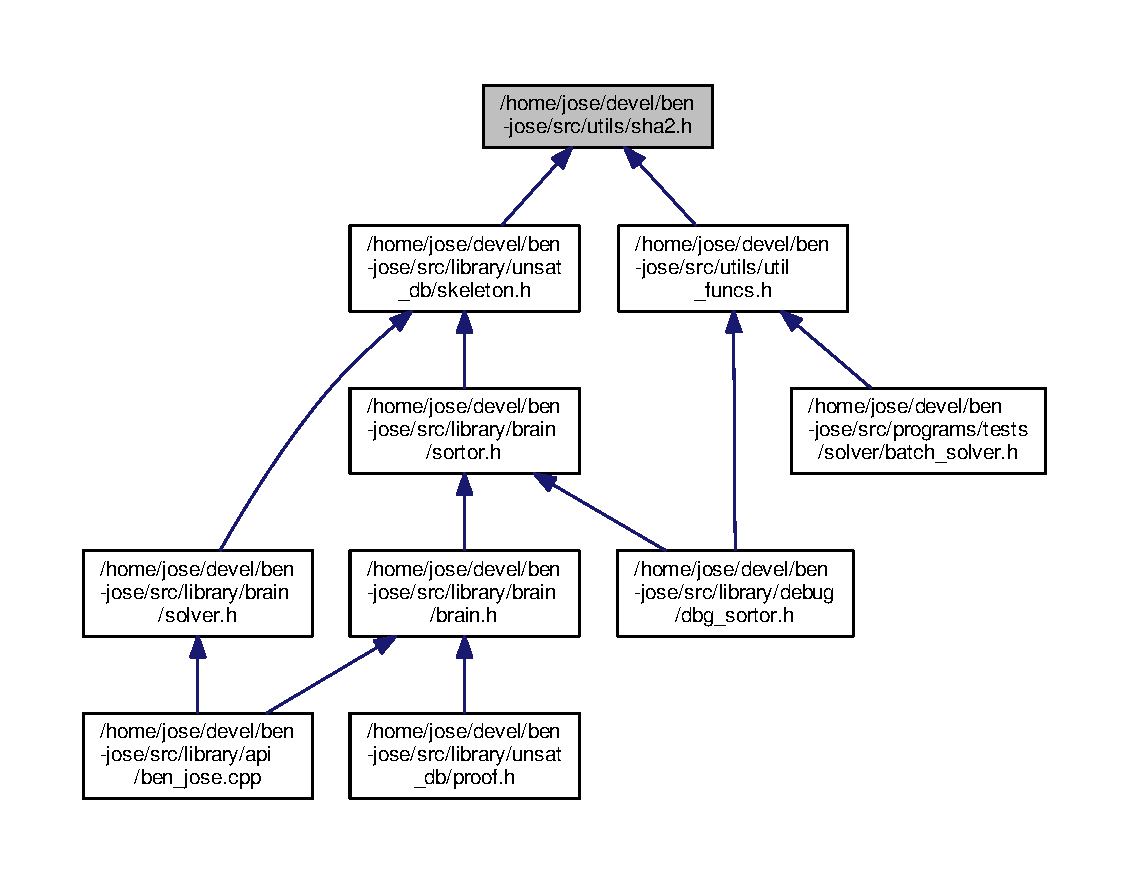
\includegraphics[width=350pt]{d7/dfb/sha2_8h__dep__incl}
\end{center}
\end{figure}
\subsection*{Classes}
\begin{DoxyCompactItemize}
\item 
struct \hyperlink{structsha2__context}{sha2\+\_\+context}
\begin{DoxyCompactList}\small\item\em S\+H\+A-\/256 context structure. \end{DoxyCompactList}\end{DoxyCompactItemize}
\subsection*{Functions}
\begin{DoxyCompactItemize}
\item 
void \hyperlink{sha2_8h_ae01444aa81c862eb74f0545b8d05371a}{sha2\+\_\+starts} (\hyperlink{structsha2__context}{sha2\+\_\+context} $\ast$ctx, int is224)
\begin{DoxyCompactList}\small\item\em S\+H\+A-\/256 context setup. \end{DoxyCompactList}\item 
void \hyperlink{sha2_8h_abe89ecad33cb50bfa16c0dbd62adbb52}{sha2\+\_\+update} (\hyperlink{structsha2__context}{sha2\+\_\+context} $\ast$ctx, unsigned char $\ast$input, int ilen)
\begin{DoxyCompactList}\small\item\em S\+H\+A-\/256 process buffer. \end{DoxyCompactList}\item 
void \hyperlink{sha2_8h_a4dbd38a93b5b61c637a8a29dd0e850f0}{sha2\+\_\+finish} (\hyperlink{structsha2__context}{sha2\+\_\+context} $\ast$ctx, unsigned char $\ast$output)
\begin{DoxyCompactList}\small\item\em S\+H\+A-\/256 final digest. \end{DoxyCompactList}\item 
void \hyperlink{sha2_8h_a3a32be6d62771a80c4baa302bf516f1d}{sha2} (unsigned char $\ast$input, int ilen, unsigned char $\ast$output, int is224)
\begin{DoxyCompactList}\small\item\em Output = S\+H\+A-\/256( input buffer ) \end{DoxyCompactList}\item 
void \hyperlink{sha2_8h_a2135b4741d1821a66ee0a2d15ae5d943}{sha2\+\_\+hmac\+\_\+starts} (\hyperlink{structsha2__context}{sha2\+\_\+context} $\ast$ctx, int is224, unsigned char $\ast$key, int keylen)
\begin{DoxyCompactList}\small\item\em Output = S\+H\+A-\/256( file contents ) \end{DoxyCompactList}\item 
void \hyperlink{sha2_8h_a5a0a7c2628e73dded8df2e530717a99a}{sha2\+\_\+hmac\+\_\+update} (\hyperlink{structsha2__context}{sha2\+\_\+context} $\ast$ctx, unsigned char $\ast$input, int ilen)
\begin{DoxyCompactList}\small\item\em S\+H\+A-\/256 H\+M\+AC process buffer. \end{DoxyCompactList}\item 
void \hyperlink{sha2_8h_a26eb68bd8099e178f5110e6437596777}{sha2\+\_\+hmac\+\_\+finish} (\hyperlink{structsha2__context}{sha2\+\_\+context} $\ast$ctx, unsigned char $\ast$output)
\begin{DoxyCompactList}\small\item\em S\+H\+A-\/256 H\+M\+AC final digest. \end{DoxyCompactList}\item 
void \hyperlink{sha2_8h_a33f96332050976275e169a7a676d703f}{sha2\+\_\+hmac} (unsigned char $\ast$key, int keylen, unsigned char $\ast$input, int ilen, unsigned char $\ast$output, int is224)
\begin{DoxyCompactList}\small\item\em Output = H\+M\+A\+C-\/\+S\+H\+A-\/256( hmac key, input buffer ) \end{DoxyCompactList}\item 
int \hyperlink{sha2_8h_a8a7026f38413c81e28966631a8dbc004}{sha2\+\_\+self\+\_\+test} (int verbose)
\begin{DoxyCompactList}\small\item\em Checkup routine. \end{DoxyCompactList}\end{DoxyCompactItemize}


\subsection{Function Documentation}
\index{sha2.\+h@{sha2.\+h}!sha2\+\_\+starts@{sha2\+\_\+starts}}
\index{sha2\+\_\+starts@{sha2\+\_\+starts}!sha2.\+h@{sha2.\+h}}
\subsubsection[{\texorpdfstring{sha2\+\_\+starts(sha2\+\_\+context $\ast$ctx, int is224)}{sha2_starts(sha2_context *ctx, int is224)}}]{\setlength{\rightskip}{0pt plus 5cm}void sha2\+\_\+starts (
\begin{DoxyParamCaption}
\item[{{\bf sha2\+\_\+context} $\ast$}]{ctx, }
\item[{int}]{is224}
\end{DoxyParamCaption}
)}\hypertarget{sha2_8h_ae01444aa81c862eb74f0545b8d05371a}{}\label{sha2_8h_ae01444aa81c862eb74f0545b8d05371a}


S\+H\+A-\/256 context setup. 


\begin{DoxyParams}{Parameters}
{\em ctx} & context to be initialized \\
\hline
{\em is224} & 0 = use S\+H\+A256, 1 = use S\+H\+A224 \\
\hline
\end{DoxyParams}


Here is the caller graph for this function\+:
\nopagebreak
\begin{figure}[H]
\begin{center}
\leavevmode
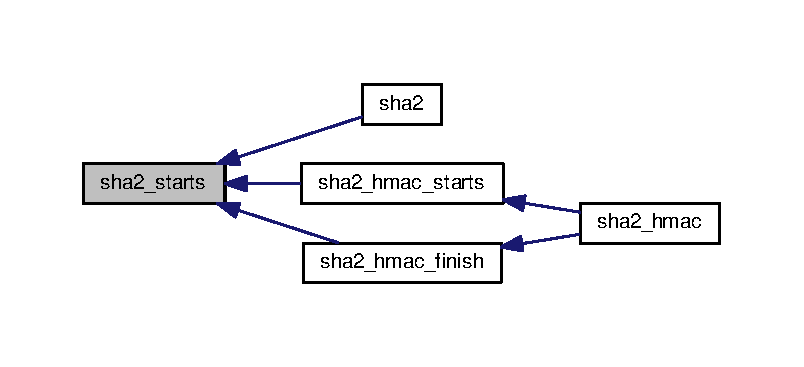
\includegraphics[width=350pt]{db/d4d/sha2_8h_ae01444aa81c862eb74f0545b8d05371a_icgraph}
\end{center}
\end{figure}


\index{sha2.\+h@{sha2.\+h}!sha2\+\_\+update@{sha2\+\_\+update}}
\index{sha2\+\_\+update@{sha2\+\_\+update}!sha2.\+h@{sha2.\+h}}
\subsubsection[{\texorpdfstring{sha2\+\_\+update(sha2\+\_\+context $\ast$ctx, unsigned char $\ast$input, int ilen)}{sha2_update(sha2_context *ctx, unsigned char *input, int ilen)}}]{\setlength{\rightskip}{0pt plus 5cm}void sha2\+\_\+update (
\begin{DoxyParamCaption}
\item[{{\bf sha2\+\_\+context} $\ast$}]{ctx, }
\item[{unsigned char $\ast$}]{input, }
\item[{int}]{ilen}
\end{DoxyParamCaption}
)}\hypertarget{sha2_8h_abe89ecad33cb50bfa16c0dbd62adbb52}{}\label{sha2_8h_abe89ecad33cb50bfa16c0dbd62adbb52}


S\+H\+A-\/256 process buffer. 


\begin{DoxyParams}{Parameters}
{\em ctx} & S\+H\+A-\/256 context \\
\hline
{\em input} & buffer holding the data \\
\hline
{\em ilen} & length of the input data \\
\hline
\end{DoxyParams}


Here is the caller graph for this function\+:
\nopagebreak
\begin{figure}[H]
\begin{center}
\leavevmode
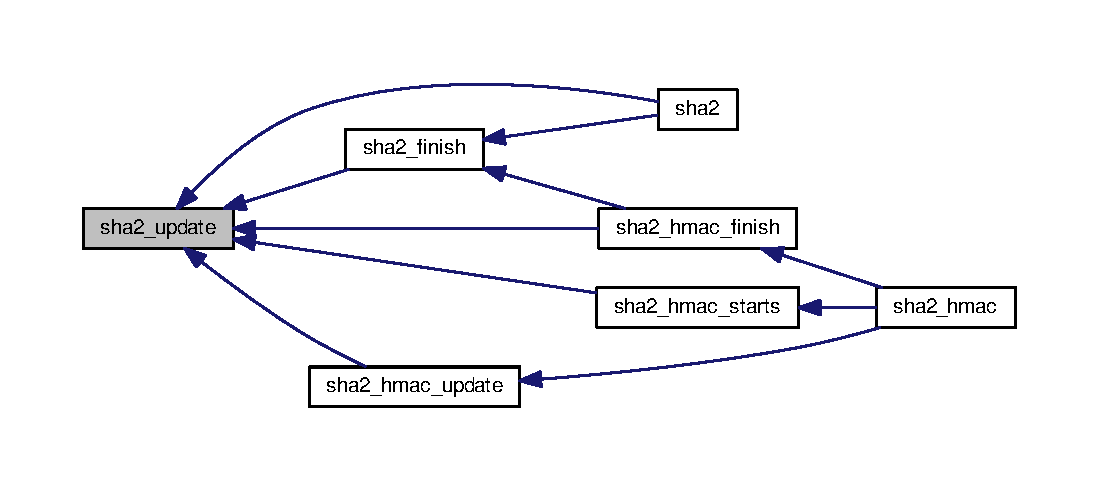
\includegraphics[width=350pt]{db/d4d/sha2_8h_abe89ecad33cb50bfa16c0dbd62adbb52_icgraph}
\end{center}
\end{figure}


\index{sha2.\+h@{sha2.\+h}!sha2\+\_\+finish@{sha2\+\_\+finish}}
\index{sha2\+\_\+finish@{sha2\+\_\+finish}!sha2.\+h@{sha2.\+h}}
\subsubsection[{\texorpdfstring{sha2\+\_\+finish(sha2\+\_\+context $\ast$ctx, unsigned char $\ast$output)}{sha2_finish(sha2_context *ctx, unsigned char *output)}}]{\setlength{\rightskip}{0pt plus 5cm}void sha2\+\_\+finish (
\begin{DoxyParamCaption}
\item[{{\bf sha2\+\_\+context} $\ast$}]{ctx, }
\item[{unsigned char $\ast$}]{output}
\end{DoxyParamCaption}
)}\hypertarget{sha2_8h_a4dbd38a93b5b61c637a8a29dd0e850f0}{}\label{sha2_8h_a4dbd38a93b5b61c637a8a29dd0e850f0}


S\+H\+A-\/256 final digest. 


\begin{DoxyParams}{Parameters}
{\em ctx} & S\+H\+A-\/256 context \\
\hline
{\em output} & S\+H\+A-\/224/256 checksum result \\
\hline
\end{DoxyParams}


Here is the call graph for this function\+:
\nopagebreak
\begin{figure}[H]
\begin{center}
\leavevmode
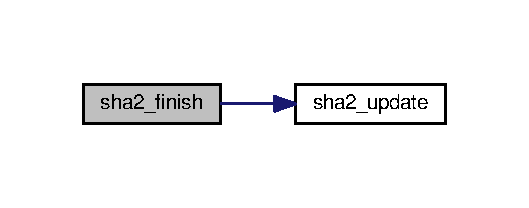
\includegraphics[width=254pt]{db/d4d/sha2_8h_a4dbd38a93b5b61c637a8a29dd0e850f0_cgraph}
\end{center}
\end{figure}




Here is the caller graph for this function\+:
\nopagebreak
\begin{figure}[H]
\begin{center}
\leavevmode
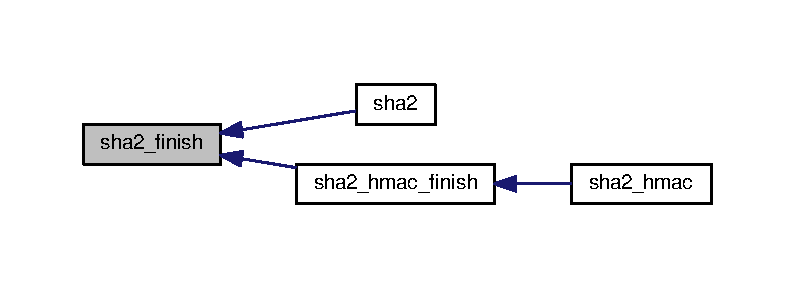
\includegraphics[width=350pt]{db/d4d/sha2_8h_a4dbd38a93b5b61c637a8a29dd0e850f0_icgraph}
\end{center}
\end{figure}


\index{sha2.\+h@{sha2.\+h}!sha2@{sha2}}
\index{sha2@{sha2}!sha2.\+h@{sha2.\+h}}
\subsubsection[{\texorpdfstring{sha2(unsigned char $\ast$input, int ilen, unsigned char $\ast$output, int is224)}{sha2(unsigned char *input, int ilen, unsigned char *output, int is224)}}]{\setlength{\rightskip}{0pt plus 5cm}void sha2 (
\begin{DoxyParamCaption}
\item[{unsigned char $\ast$}]{input, }
\item[{int}]{ilen, }
\item[{unsigned char $\ast$}]{output, }
\item[{int}]{is224}
\end{DoxyParamCaption}
)}\hypertarget{sha2_8h_a3a32be6d62771a80c4baa302bf516f1d}{}\label{sha2_8h_a3a32be6d62771a80c4baa302bf516f1d}


Output = S\+H\+A-\/256( input buffer ) 


\begin{DoxyParams}{Parameters}
{\em input} & buffer holding the data \\
\hline
{\em ilen} & length of the input data \\
\hline
{\em output} & S\+H\+A-\/224/256 checksum result \\
\hline
{\em is224} & 0 = use S\+H\+A256, 1 = use S\+H\+A224 \\
\hline
\end{DoxyParams}


Here is the call graph for this function\+:
\nopagebreak
\begin{figure}[H]
\begin{center}
\leavevmode
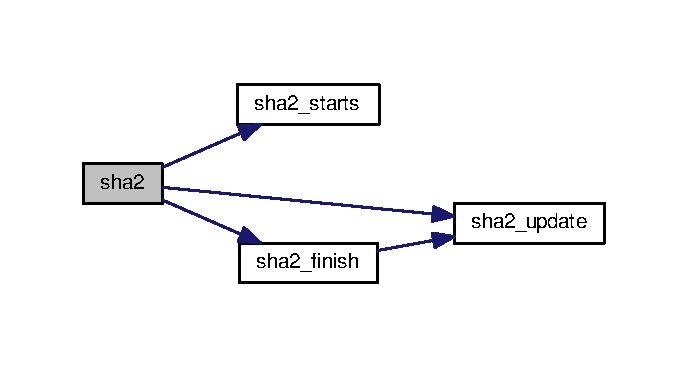
\includegraphics[width=330pt]{db/d4d/sha2_8h_a3a32be6d62771a80c4baa302bf516f1d_cgraph}
\end{center}
\end{figure}


\index{sha2.\+h@{sha2.\+h}!sha2\+\_\+hmac\+\_\+starts@{sha2\+\_\+hmac\+\_\+starts}}
\index{sha2\+\_\+hmac\+\_\+starts@{sha2\+\_\+hmac\+\_\+starts}!sha2.\+h@{sha2.\+h}}
\subsubsection[{\texorpdfstring{sha2\+\_\+hmac\+\_\+starts(sha2\+\_\+context $\ast$ctx, int is224, unsigned char $\ast$key, int keylen)}{sha2_hmac_starts(sha2_context *ctx, int is224, unsigned char *key, int keylen)}}]{\setlength{\rightskip}{0pt plus 5cm}void sha2\+\_\+hmac\+\_\+starts (
\begin{DoxyParamCaption}
\item[{{\bf sha2\+\_\+context} $\ast$}]{ctx, }
\item[{int}]{is224, }
\item[{unsigned char $\ast$}]{key, }
\item[{int}]{keylen}
\end{DoxyParamCaption}
)}\hypertarget{sha2_8h_a2135b4741d1821a66ee0a2d15ae5d943}{}\label{sha2_8h_a2135b4741d1821a66ee0a2d15ae5d943}


Output = S\+H\+A-\/256( file contents ) 


\begin{DoxyParams}{Parameters}
{\em path} & input file name \\
\hline
{\em output} & S\+H\+A-\/224/256 checksum result \\
\hline
{\em is224} & 0 = use S\+H\+A256, 1 = use S\+H\+A224\\
\hline
\end{DoxyParams}
\begin{DoxyReturn}{Returns}
0 if successful, 1 if fopen failed, or 2 if fread failed S\+H\+A-\/256 H\+M\+AC context setup
\end{DoxyReturn}

\begin{DoxyParams}{Parameters}
{\em ctx} & H\+M\+AC context to be initialized \\
\hline
{\em is224} & 0 = use S\+H\+A256, 1 = use S\+H\+A224 \\
\hline
{\em key} & H\+M\+AC secret key \\
\hline
{\em keylen} & length of the H\+M\+AC key \\
\hline
\end{DoxyParams}


Here is the call graph for this function\+:
\nopagebreak
\begin{figure}[H]
\begin{center}
\leavevmode
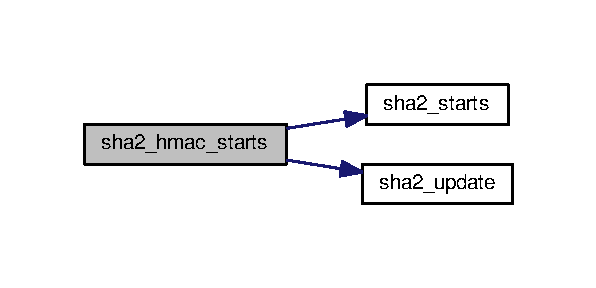
\includegraphics[width=286pt]{db/d4d/sha2_8h_a2135b4741d1821a66ee0a2d15ae5d943_cgraph}
\end{center}
\end{figure}




Here is the caller graph for this function\+:
\nopagebreak
\begin{figure}[H]
\begin{center}
\leavevmode
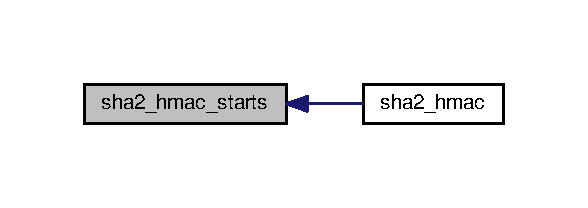
\includegraphics[width=282pt]{db/d4d/sha2_8h_a2135b4741d1821a66ee0a2d15ae5d943_icgraph}
\end{center}
\end{figure}


\index{sha2.\+h@{sha2.\+h}!sha2\+\_\+hmac\+\_\+update@{sha2\+\_\+hmac\+\_\+update}}
\index{sha2\+\_\+hmac\+\_\+update@{sha2\+\_\+hmac\+\_\+update}!sha2.\+h@{sha2.\+h}}
\subsubsection[{\texorpdfstring{sha2\+\_\+hmac\+\_\+update(sha2\+\_\+context $\ast$ctx, unsigned char $\ast$input, int ilen)}{sha2_hmac_update(sha2_context *ctx, unsigned char *input, int ilen)}}]{\setlength{\rightskip}{0pt plus 5cm}void sha2\+\_\+hmac\+\_\+update (
\begin{DoxyParamCaption}
\item[{{\bf sha2\+\_\+context} $\ast$}]{ctx, }
\item[{unsigned char $\ast$}]{input, }
\item[{int}]{ilen}
\end{DoxyParamCaption}
)}\hypertarget{sha2_8h_a5a0a7c2628e73dded8df2e530717a99a}{}\label{sha2_8h_a5a0a7c2628e73dded8df2e530717a99a}


S\+H\+A-\/256 H\+M\+AC process buffer. 


\begin{DoxyParams}{Parameters}
{\em ctx} & H\+M\+AC context \\
\hline
{\em input} & buffer holding the data \\
\hline
{\em ilen} & length of the input data \\
\hline
\end{DoxyParams}


Here is the call graph for this function\+:
\nopagebreak
\begin{figure}[H]
\begin{center}
\leavevmode
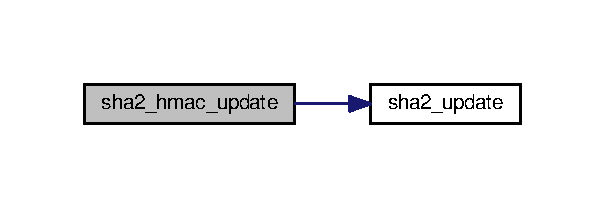
\includegraphics[width=290pt]{db/d4d/sha2_8h_a5a0a7c2628e73dded8df2e530717a99a_cgraph}
\end{center}
\end{figure}




Here is the caller graph for this function\+:
\nopagebreak
\begin{figure}[H]
\begin{center}
\leavevmode
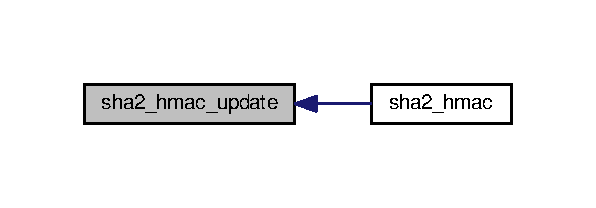
\includegraphics[width=286pt]{db/d4d/sha2_8h_a5a0a7c2628e73dded8df2e530717a99a_icgraph}
\end{center}
\end{figure}


\index{sha2.\+h@{sha2.\+h}!sha2\+\_\+hmac\+\_\+finish@{sha2\+\_\+hmac\+\_\+finish}}
\index{sha2\+\_\+hmac\+\_\+finish@{sha2\+\_\+hmac\+\_\+finish}!sha2.\+h@{sha2.\+h}}
\subsubsection[{\texorpdfstring{sha2\+\_\+hmac\+\_\+finish(sha2\+\_\+context $\ast$ctx, unsigned char $\ast$output)}{sha2_hmac_finish(sha2_context *ctx, unsigned char *output)}}]{\setlength{\rightskip}{0pt plus 5cm}void sha2\+\_\+hmac\+\_\+finish (
\begin{DoxyParamCaption}
\item[{{\bf sha2\+\_\+context} $\ast$}]{ctx, }
\item[{unsigned char $\ast$}]{output}
\end{DoxyParamCaption}
)}\hypertarget{sha2_8h_a26eb68bd8099e178f5110e6437596777}{}\label{sha2_8h_a26eb68bd8099e178f5110e6437596777}


S\+H\+A-\/256 H\+M\+AC final digest. 


\begin{DoxyParams}{Parameters}
{\em ctx} & H\+M\+AC context \\
\hline
{\em output} & S\+H\+A-\/224/256 H\+M\+AC checksum result \\
\hline
\end{DoxyParams}


Here is the call graph for this function\+:
\nopagebreak
\begin{figure}[H]
\begin{center}
\leavevmode
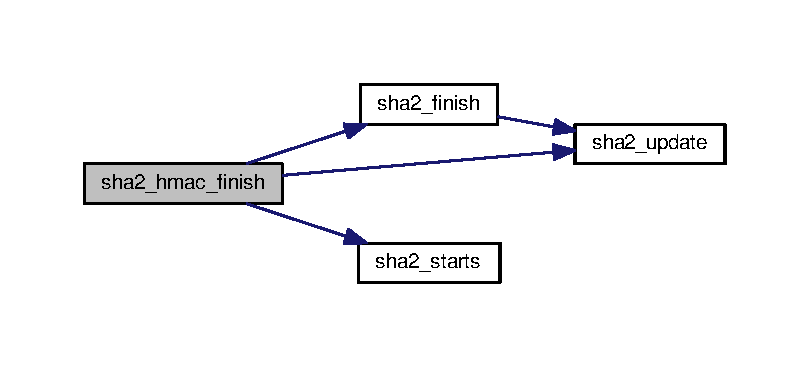
\includegraphics[width=350pt]{db/d4d/sha2_8h_a26eb68bd8099e178f5110e6437596777_cgraph}
\end{center}
\end{figure}




Here is the caller graph for this function\+:
\nopagebreak
\begin{figure}[H]
\begin{center}
\leavevmode
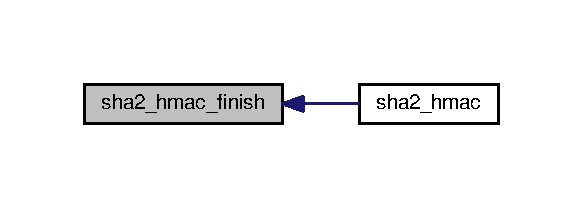
\includegraphics[width=280pt]{db/d4d/sha2_8h_a26eb68bd8099e178f5110e6437596777_icgraph}
\end{center}
\end{figure}


\index{sha2.\+h@{sha2.\+h}!sha2\+\_\+hmac@{sha2\+\_\+hmac}}
\index{sha2\+\_\+hmac@{sha2\+\_\+hmac}!sha2.\+h@{sha2.\+h}}
\subsubsection[{\texorpdfstring{sha2\+\_\+hmac(unsigned char $\ast$key, int keylen, unsigned char $\ast$input, int ilen, unsigned char $\ast$output, int is224)}{sha2_hmac(unsigned char *key, int keylen, unsigned char *input, int ilen, unsigned char *output, int is224)}}]{\setlength{\rightskip}{0pt plus 5cm}void sha2\+\_\+hmac (
\begin{DoxyParamCaption}
\item[{unsigned char $\ast$}]{key, }
\item[{int}]{keylen, }
\item[{unsigned char $\ast$}]{input, }
\item[{int}]{ilen, }
\item[{unsigned char $\ast$}]{output, }
\item[{int}]{is224}
\end{DoxyParamCaption}
)}\hypertarget{sha2_8h_a33f96332050976275e169a7a676d703f}{}\label{sha2_8h_a33f96332050976275e169a7a676d703f}


Output = H\+M\+A\+C-\/\+S\+H\+A-\/256( hmac key, input buffer ) 


\begin{DoxyParams}{Parameters}
{\em key} & H\+M\+AC secret key \\
\hline
{\em keylen} & length of the H\+M\+AC key \\
\hline
{\em input} & buffer holding the data \\
\hline
{\em ilen} & length of the input data \\
\hline
{\em output} & H\+M\+A\+C-\/\+S\+H\+A-\/224/256 result \\
\hline
{\em is224} & 0 = use S\+H\+A256, 1 = use S\+H\+A224 \\
\hline
\end{DoxyParams}


Here is the call graph for this function\+:
\nopagebreak
\begin{figure}[H]
\begin{center}
\leavevmode
\includegraphics[width=350pt]{db/d4d/sha2_8h_a33f96332050976275e169a7a676d703f_cgraph}
\end{center}
\end{figure}


\index{sha2.\+h@{sha2.\+h}!sha2\+\_\+self\+\_\+test@{sha2\+\_\+self\+\_\+test}}
\index{sha2\+\_\+self\+\_\+test@{sha2\+\_\+self\+\_\+test}!sha2.\+h@{sha2.\+h}}
\subsubsection[{\texorpdfstring{sha2\+\_\+self\+\_\+test(int verbose)}{sha2_self_test(int verbose)}}]{\setlength{\rightskip}{0pt plus 5cm}int sha2\+\_\+self\+\_\+test (
\begin{DoxyParamCaption}
\item[{int}]{verbose}
\end{DoxyParamCaption}
)}\hypertarget{sha2_8h_a8a7026f38413c81e28966631a8dbc004}{}\label{sha2_8h_a8a7026f38413c81e28966631a8dbc004}


Checkup routine. 

\begin{DoxyReturn}{Returns}
0 if successful, or 1 if the test failed 
\end{DoxyReturn}


Here is the caller graph for this function\+:

%--- End generated contents ---

% Index
\newpage
\phantomsection
\addcontentsline{toc}{chapter}{Index}
\printindex

\end{document}
